% ******************************* PhD Thesis Template **************************
\documentclass[a4paper,12pt,times,numbered,print,index]{Classes/PhDThesisPSnPDF}

% ********************************** Preamble **********************************
% ******************************************************************************
% ****************************** Custom Margin *********************************

% Add `custommargin' in the document class options to use this section
% Set {innerside margin / outerside margin / topmargin / bottom margin}  and
% other page dimensions
\ifsetCustomMargin
  \RequirePackage[left=37mm,right=30mm,top=35mm,bottom=30mm]{geometry}
  \setFancyHdr % To apply fancy header after geometry package is loaded
\fi

% Add spaces between paragraphs
%\setlength{\parskip}{0.5em}
% Ragged bottom avoids extra whitespaces between paragraphs
\raggedbottom
% To remove the excess top spacing for enumeration, list and description
%\usepackage{enumitem}
%\setlist[enumerate,itemize,description]{topsep=0em}

% *****************************************************************************
% ******************* Fonts (like different typewriter fonts etc.)*************

% Add `customfont' in the document class option to use this section

\ifsetCustomFont
  % Set your custom font here and use `customfont' in options. Leave empty to
  % load computer modern font (default LaTeX font).
  %\RequirePackage{helvet}

  % For use with XeLaTeX
  %  \setmainfont[
  %    Path              = ./libertine/opentype/,
  %    Extension         = .otf,
  %    UprightFont = LinLibertine_R,
  %    BoldFont = LinLibertine_RZ, % Linux Libertine O Regular Semibold
  %    ItalicFont = LinLibertine_RI,
  %    BoldItalicFont = LinLibertine_RZI, % Linux Libertine O Regular Semibold Italic
  %  ]
  %  {libertine}
  %  % load font from system font
  %  \newfontfamily\libertinesystemfont{Linux Libertine O}
\fi

% *****************************************************************************
% **************************** Custom Packages ********************************

% ************************* Algorithms and Pseudocode **************************

%\usepackage{algpseudocode}


% ********************Captions and Hyperreferencing / URL **********************

% Captions: This makes captions of figures use a boldfaced small font.
%\RequirePackage[small,bf]{caption}

\RequirePackage[labelsep=space,tableposition=top]{caption}
\renewcommand{\figurename}{Fig.} %to support older versions of captions.sty


% *************************** Graphics and figures *****************************

%\usepackage{rotating}
%\usepackage{wrapfig}

% Uncomment the following two lines to force Latex to place the figure.
% Use [H] when including graphics. Note 'H' instead of 'h'
%\usepackage{float}
%\restylefloat{figure}

% Subcaption package is also available in the sty folder you can use that by
% uncommenting the following line
% This is for people stuck with older versions of texlive
%\usepackage{sty/caption/subcaption}
\usepackage{subcaption}

\documentclass{article}

% ********************************** Tables ************************************
\usepackage{booktabs} % For professional looking tables
\usepackage{multirow}


% *********************************** SI Units *********************************
\usepackage{siunitx} % use this package module for SI units


% ******************************* Line Spacing *********************************

% Choose linespacing as appropriate. Default is one-half line spacing as per the
% University guidelines

% \doublespacing
% \onehalfspacing
% \singlespacing


% ************************ Formatting / Footnote *******************************

% Don't break enumeration (etc.) across pages in an ugly manner (default 10000)
%\clubpenalty=500
%\widowpenalty=500

%\usepackage[perpage]{footmisc} %Range of footnote options

% ********************** References *************************
\usepackage{natbib}

% ********************** TOC depth and numbering depth *************************

\setcounter{secnumdepth}{2}
\setcounter{tocdepth}{2}


\usepackage{natbib}
\bibliographystyle{apalike}
% ************************ Thesis Information & Meta-data **********************
% Thesis title and author information, refernce file for biblatex
% ************************ Thesis Information & Meta-data **********************
%% The title of the thesis
\title{Mining Software Repositories to Determine the Impact of Team Factors on the Structural Attributes of Software}
%\texorpdfstring is used for PDF metadata. Usage:
%\texorpdfstring{LaTeX_Version}{PDF Version (non-latex)} eg.,
%\texorpdfstring{$sigma$}{sigma}

%% Subtitle (Optional)
%\subtitle{Using the CUED template}

%% The full name of the author
\author{Ahmmad Youssef}

%% Department (eg. Department of Engineering, Maths, Physics)
\dept{Department of Computer Science}

%% University and Crest
\university{Brunel University}
% Crest minimum should be 30mm.
%\crest{\includegraphics[width=0.2\textwidth]{University_Crest}}
%% Use this crest, if you are using the college crest
%% Crest long miminum should be 65mm
%\crest{\includegraphics[width=0.45\textwidth]{University_Crest_Long}}

%% College shield [optional] 
% Crest minimum should be 30mm.
\collegeshield{
\includegraphics[width=0.30\textwidth]{CollegeShields/Brunel.jpg}}


%% Supervisor (optional)
%% for multiple supervisors, append each supervisor with the \newline command
\supervisor{Dr. Andrea Capiluppi\newline
Professor. Tracy Hall}

%% Supervisor Role (optional) - Supervisor (default) or advisor
% \supervisorrole{\textbf{Supervisors: }}
%% if no title is desired:
% \supervisorrole{}

%% Supervisor line width: required to align supervisors
%\supervisorlinewidth{0.35\textwidth}

%% Advisor (optional)
%% for multiple advisors, append each advisor with the \newline command
%\advisor{Dr. A. Advisor\newline
%Dr. B. Advisor}
     
%% Advisor Role (optional) - Advisor (default) or leave empty
% \advisorrole{Advisors: }
%% if no title is required
% \advisorrole{}

%% Advisor line width: required to align supervisors
%\advisorlinewidth{0.25\textwidth}


%% You can redefine the submission text:
% Default as per the University guidelines:
% ``This dissertation is submitted for the degree of''
%\renewcommand{\submissiontext}{change the default text here if needed}

%% Full title of the Degree
\degreetitle{Doctor of Philosophy}

%% College affiliation (optional)
\college{}

%% Submission date
% Default is set as {\monthname[\the\month]\space\the\year}
%\degreedate{July 2018} 

%% Meta information
\subject{LaTeX} \keywords{{LaTeX} {PhD Thesis} {Engineering} {Brunel University}}


% ******************************** Front Matter ********************************
\begin{document}

\frontmatter
\maketitle

\setlength{\parindent}{0em}
\setlength{\parskip}{2ex}
% ******************************* Thesis Dedidcation ********************************

\begin{dedication} 

Dedication to be completed.

\end{dedication}


% ******************************* Thesis Declaration ***************************

\begin{declaration}

I hereby declare...

% Author and date will be inserted automatically from thesis.tex \author \degreedate

\end{declaration}


% ************************** Thesis Acknowledgements **************************

\begin{acknowledgements}      


Acknowledgements to be completed.

\end{acknowledgements}

% ************************** Thesis Abstract *****************************
% Use `abstract' as an option in the document class to print only the titlepage and the abstract.
\begin{abstract}

As per the definition of socio-technical systems, the role of 'people' in software projects is a well-known factor for their long-term, sustainable success. The size and the stability of a software development team are the often cited attributes in the 'people' category as being of greatest significance to stakeholders. Team size is usually considered as a measure of the number of developers that modify a project source code; while team stability is typically the cumulative time that each team member has worked with their fellow team members.

The impact of inappropriately sized or less stable teams can have profound effects on budget and time-scales: given that up to 80\% of development budgets are consumed in the maintenance phase of the lifecycle, these team-building factors are among the key aspects in a software project. While existing research establishes correlations between the size and stability of the development team and software fault-proneness, there is limited research investigating the impact on maintainability. Therefore, it is essential to gain an insight into how these aspects of team composition influence and are influenced by the internal characteristics of a software project, that inevitably drive the maintenance costs of software. 

Within this research the GoogleCode open-source forge is mined and, using the Chidamber and Kemerer design metrics suite, the impact of development team size and stability on the internal structural attributes of software is isolated and quantified. Drawing on prior research correlating these internal attributes with external attributes, the impact on maintainability is deduced and insight is given to the structural aspects that drive the increased fault-proneness that previous research has associated with larger, less stable development teams. Of these internal structural attributes, it is found that some measures of modularity are enhanced when comparing projects developed by smaller teams with those developed by larger teams; while measures of cohesion and complexity are degraded. Likewise, similar observations are made when projects authored by newly formed development teams are compared with those from teams exhibiting continuity spanning across projects.
\end{abstract}


% *********************** Adding TOC and List of Figures ***********************

\setlength{\parskip}{0ex}
\tableofcontents
\listoffigures
\listoftables
%\printnomenclature

% ******************************** Main Matter *********************************
\mainmatter
\setlength{\parskip}{2ex}
%!TEX root = ../thesis.tex

\graphicspath{{Chapter1/Figures/}{Chapter1/Tables/}{Chapter1/Charts/}}

\chapter{Introduction}

\section{Research Context} %Section - 1.1 
There are many critical decisions that face software development practitioners throughout the development lifecycle, and that ultimately can contribute to the success or failure of a project. These decisions, broadly, fall under the categories of Process, Technology, or People \citep{nasir2011critical}. Decisions in the Process category are those such as the choice of development methodology\citep{chow2008survey}, development standards \citep{rainer2002key}, or the decision to invest in test automation to achieve shorter testing cycles \citep{lewis2016software}. Technology decisions can vary from questions of what hardware or programming languages to use for development to the selection of tools that development teams should employ \citep{scheer2000enterprise}. Finally, the People category of decisions focuses on issues such as the resourcing and staffing of software development project teams and how those teams fit into the wider organisation \citep{krishnan1998role}.

Each of these categories of decisions has seen a great deal of academic research. In the Process category Kuhrmann et al \citep{kuhrmann2015software} conducted a mapping study of the field of software process improvement, finding 635 publications over the past 25 years. To give a flavour of these studies, some investigate how greater adherence to established software process models such as CMM \citep{paulk1993capability} or ISO \citep{ISO15504} can result in better quality \citep{harter2012does, abrahamsson2013measuring}. Others are case studies on how organisations manage adoption of process models and refinements are suggested for particular contexts such as small or medium enterprises \citep{sulayman2012software, balla2001quality}. Research in Technology category is extremely broad covers topics such as the suitability of particular technologies for a given use \citep{sharp2003evaluating, baker2006real}, the security implications of using a given technology stack \citep{gangwar2014web, mirheidari2012two, choukse2012developing}, or studies of the tools that can be used to facilitate team communication in a global context \citep{portillo2012tools}. Finally, in the People category the studies, again broad and diverse, can vary from a study of what motivates Open Source Software contributors \citep{von2012carrots} through to the impact of team size or team diversity on team performance \citep{hoch2010most}. 

Of these three categories, 'People' decisions are established to have the greatest impact on development team productivity \citep{trendowicz2009factors} and critical success factors for software development projects are, by far, more likely to be in the realm of people factors \citep{boehm1978characteristics}. Software development is intrinsically a human activity and a more people-oriented approach is in the ascendency evident in, amongst other things, increasing adoption of agile methodologies \citep{pirzadeh2010human}.

Nasir et al \citep{nasir2011critical} conducted an extensive literature survey of the critical success factors that impact software projects finding that in the People category some of the most cited project success factors, based on industrial case studies as well as surveys, relate specifically to the composition of the software development team \citep{schmidt2001identifying, kappelman2006early, humphrey2005big, glass2006standish, sauer2003state}. This is pertinent because within most real world enterprise software development projects, 'people' decisions such as those around the composition of individual development teams can be made by managers who are not particularly senior and, indeed, possibly even with input from individual developers. By contrast, location strategies or project budgets are often dictated by senior management with little or no influence from those lower in the management chain and are therefore in the within the sphere of influence of significantly fewer practitioners. When considering decentralised volunteer-based Free Libre Open Source (FLOSS) projects, it is also true that, beyond the composition of the software development team, there can be limited tools with which stakeholders can influence the success or failure of a project \citep{schweik2008brooks}.

In the context of this research, team size is a measure of the number of developers that modify a project source code; while team stability is a measure of the cumulative time that each team member has worked with their fellow team members. Within the 'People' category of research there is an extensive body of work that empirically proves that team size and stability are linked to project success rates, team productivity, and external attributes such as fault-proneness. As detailed in the chapter titled 'Related Work', earlier research found that smaller, more stable development teams are more productive, produce less fault-prone software, and have higher levels of stakeholder satisfaction.  Much of this research has been motivated, at least in part, to help inform practitioners how to compose their own development teams so that the associated risks were limited as far as practicable, recognising that team composition is one of the few levers within the grasp of management to strongly influence project outcomes. 

The research asserts that new insights can be gained into how team size and stability impact the produced software by measuring the internal attributes of the software instead of the more traditional approach of measuring its external attributes. Through this approach practitioners can form a more complete picture to inform decision-making. Uniquely, this also enables practitioners to measure and monitor key indicators, taking remedial action at earlier stages in the development lifecycle.

\section{Team Size and Stability in the Literature} %Section - 1.2
In 1974 Fred Brooks, in his popular book 'The Mythical Man Month'\citep{brooks1986mythical}, stated that adding additional developers to a project can result in a loss of productivity due to the exponential difficulties involved in maintaining effective communication within a larger team. In 2000, Eric Raymond, in his book 'The Cathedral and the Bazaar', asserted that in open source software development larger development teams are more effective at identifying and resolving bugs, leading to less fault-prone software. Raymond termed this 'Linus Law' named after the lead linux developer. In contrast to both Brooks and Linus law is the 'Core Team principle' that states that the size of a team should not have an impact on the success of the project as core development groups are always small. For researchers or practitioners, attempting to navigate these somewhat conflicting principles to understand which factors will win out is no easy task \citep{schweik2008brooks}. 

Greater consensus is evident when reviewing the literature around team stability - a significantly smaller body of work - which agrees that more stable teams produce less fault-prone software. One particularly stark observation, from Huckman et al\citep{huckman2009team}, was that, as team stability increased by 50\% and defects decreased by 19\%.

Questions of how development team size and stability impact fault-proneness is also very much at the forefront of practitioner minds. Many practitioners have taken the time to present their evidence and document their experience around these two particular strands in whitepapers and blog posts, generally agreeing with the academic research - some through empirical means \citep{mcconnell2017less, macheronne2013critical}, others purely anecdotal \citep{erickson2012are, meccia2015critical, miller2006critical, plowman2015seven} - that smaller, more stable teams produce less fault-prone software. This is covered in more detail in Related Work.

Interest in fault-proneness is not without good reason. There are numerous examples of software faults causing governmental or corporate institutions severe reputational damage. Knight Capital is oft-cited as dramatic example how a defect in their order routing software caused a \$465 million trading loss \citep{sec2013}. Behind the headline grabbing incidents is a more pervasive issue throughout the industry. A 2003 study commissioned by the US Department of Commerce found that software bugs cost the US economy alone \$59.5 billion annually and this has only increased since. 

However, fault-proneness is not the only aspect that of concern to stakeholders. Maintainability has also seen a significant research activity. This refers to the ease with which a software system or component can be modified to correct faults, improve performance or other attributes, or adapt to a changed environment \citep{radatz1990ieee}. ISO 9126 \citep{ISO9126} states that maintainability is comprised of four sub-attributes - analysability, changeability, stability, and testability. Highly analysable software requires lower effort to investigate and understand sections of the codebase in order to remediate defects or to adapt the codebase to new requirements. Similarly, high levels of changeability require less effort to implement changes in the codebase. Stability implies a lower likelihood that making changes to the software may have unintended negative impacts. Finally, testability is a measure of the effort required to adequately test software. Taken together, a codebase exhibiting high-levels of each of these sub-attributes of maintainability support a more adaptable business against a backdrop of an oft-changing competitive landscape. 

It is of crucial importance that researchers and practitioners alike understand the impact of any factors that can have a material impact on the maintainability of software. The focus of this thesis is to add evidence and insights on how the �team size� and �team stability� play a role as factors in the maintainability of software.

\section{Internal and external factors in the literature} %Section - 1.3
Figure~\ref{fig:PeopleInternalExternal} depicts, at a very high-level, the relationship that existing literature has established between the internal structural attributes of software and its maintainability.

Prior research has focused on establishing mathematical models that describe the impact of the internal attributes of software on its external attributes including maintainability. In these models the internal attributes are the independent variables while the external attributes are the dependent variables. Broadly, these models establish that lower coupling and complexity are more favourable structural properties, leading to lower fault proneness and greater maintainability. Conversely, higher cohesion and modularity are associated with that same favourable outcome of lower fault proneness and greater maintainability. Tables 2.2 and 2.4 neatly summarise these relationships which will be detailed in the next chapter titled 'Related Work'. 

This work takes an alternative yet complementary approach to the existing body of research. The research questions in this thesis centre around establishing the impact of team composition on the internal attributes of software, essentially treating the team factors as the independent variables and the internal attributes as the dependent variables. Using the aforementioned models from existing research, these observations are subsequently used to deduce the likely impact of these team factors on maintainability. Given the breadth of the work modelling the impact of internal attributes on external attributes, this could be used to apply the observations in this research to several other external attributes.

\begin{figure}[htbp!] 
\centering    
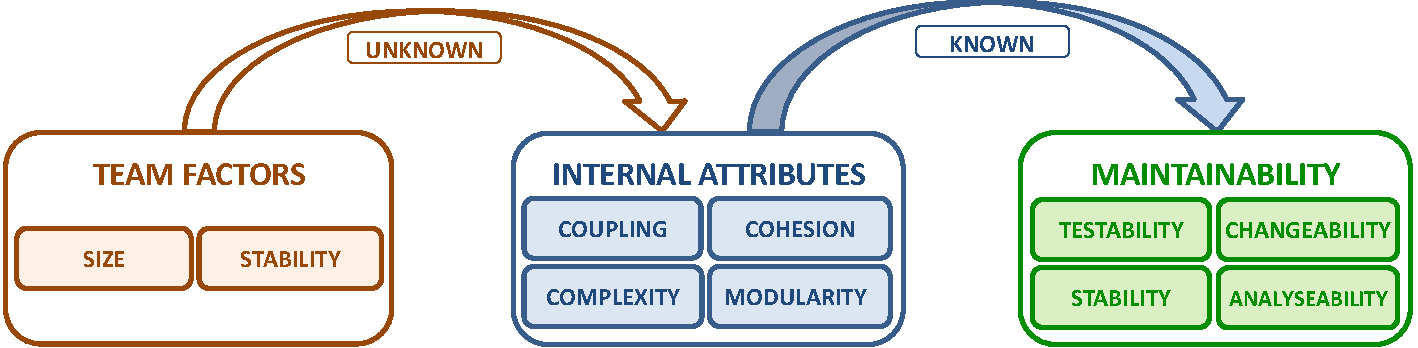
\includegraphics[width=1.0\textwidth]{PeopleInternalExternal.pdf}
\caption[People factors impacting internal attributes which, in turn, drive external attributes]{People factors can impact internal attributes which, in turn, drive external attributes}
\label{fig:PeopleInternalExternal}
\end{figure}

\section{Research Problem and Approach} %Section - 1.4
When organisations are tasked with delivering business critical software, they are often faced with multiple options to resource the project. These options could include externally recruiting a number of developers from the market and forming a new team or alternatively seconding an existing stable team comprised of developers with prior experience of working together - either from within the organisation or from an external software consultancy. 

After reviewing the existing research which does correlate team size and stability with fault-proneness it is notable that no insight is gained into how the internal attributes of software - such as coupling, cohesion, complexity and modularity - are impacted through these aspects of team composition. Given that the internal attributes of software essentially drive the aforementioned externally observable attributes (amongst others), it follows that, by all rights, this should be a crucial area of study, through which researchers can drive a deeper understanding of the impact of team composition on the aspects of stakeholder relevance such as fault-proneness and maintainability. The current state of research leaves academics and practitioners alike to draw their own conclusions on what changed internal attributes could be driving any externally observable attributes - and whether, for example, increased likelihood of fault-proneness could be observed at an earlier stage in the development lifecycle at the code level and consequently mitigated.  As Fenton rightly points out \citep{fenton2014software} practitioners are accustomed to measuring and monitoring internal attributes throughout the development process, and hence would be well placed to monitor and mitigate risks if they were broadly observable.

In order to qualitatively or quantitatively assess the negative effect of inappropriately sized or unstable teams, as for instance in the scenarios above, it is essential that we can understand the impact that team size and stability have on the sub-attributes of maintainability. Such research is essential to providing practitioners with a more complete picture to inform their decisions around team composition. While existing research informs us that more stable development teams produce less fault-proneness, understanding the impact on the analysability, changeability, testability and stability of the software, enabling practitioners to draw insights on how team stability would impact the maintainability phase of the project. This would empower practitioners to make team composition decisions that are more likely to be aligned with business goals and increase the likelihood that the project is successful. 

The empirical approach of this thesis is to measure the impact of team size and stability on the internal attributes of a software system that in turn, has a proven impact on its maintainability. This is illustrated by Figure~\ref{fig:PeopleInternalExternal}: by measuring the impact that the 'team size' and 'stability' factors play on the internal attributes of a software system, this work poses an indirect link between the people factors and the maintainability of such a system. The primary contribution of this thesis is to add to the existing body of work and to add evidence in the form of trends, correlations and models describing the relationship between team size and team stability with the produced software's internal attributes, complementing the previously established trends relating internal and external attributes as summarised in Table ~\ref{tab:PriorArtSummary} and discussed in detail in 'Related Work'.  

This research draws upon a formally popular FLOSS 'forge' - a centralised online system with tools to enable distributed development teams to work together - to provide a data set which can be mined for observations to drive the empirical work in this thesis.

\begin{table}
\captionof{table}{Summary of the relationship between structural attributes and the externally observable attributes of software, as established in the prior art.}
\begin{tabular}
 \centering
 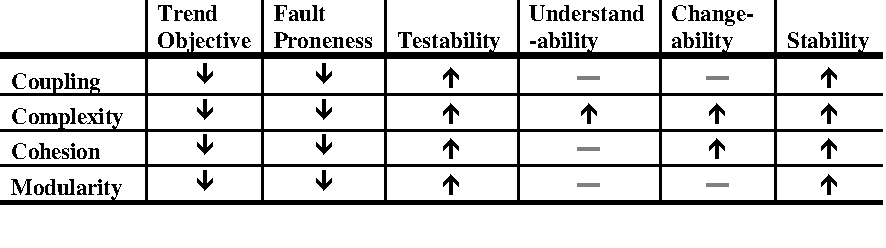
\includegraphics{PriorArtSummary.pdf}
 \label{tab:PriorArtSummary}
\end{tabular}
\end{table}
\section{Research Questions and Hypotheses} %Section - 1.5
Based on the survey of the related literature, the research questions focus on the two strands highlighted in the previously stated research problem. For each research question the null and alternative hypotheses are stated below.

\begin{itemize}
\item  \textbf{RQ1} \textit{What is the impact of development team size on the internal structural attributes of software projects and what are the implications on its maintainability?}
\begin{itemize}
\item \textbf{H0,1} \textit{Development team size does not impact the coupling, complexity, cohesion or modularity of the produced software.} Naturally the default starting position is to hypothesize that there is no relationship between team size and the structural attributes of software. 
\item \textbf{H1,1.1} \textit{Larger development teams produce software which exhibits greater coupling and complexity and lower cohesion and modularity when compared to smaller development teams.} Given existing research detailing the challenges that larger teams face in communication \citep{brooks1986mythical} and given the body of empirical research that finds that larger teams produce more fault prone software \citep{weyuker2008too, foucault2015usefulness, meneely2009secure, nagappan2008influence}, it follows that a reasonable hypothesis is that the internal structural attributes of the software produced by such a team will trend in a way that is typical of increasing fault-proneness; namely greater coupling and complexity, and lower cohesion and modularity. As both Linus law and the Core Team principle indicate the presence of forces that may ultimately work in favour of larger teams, such a hypothesis can only be proposed cautiously.
\item \textbf{H1,1.2} \textit{Larger development teams will produce less maintainable software when compared to smaller development teams.} As discussed in Related Work in detail, cohesion is correlated with testability \citep{badri2011empirical} and analysability \citep{boehm1978characteristics}, coupling and complexity has been negatively correlated with stability \citep{elish2003investigation}. Given the previous hypothesis (H0,1) that larger teams will produce software which exhibits greater coupling and complexity and lower cohesion and modularity, the hypothesis follows that maintainability will likely deteriorate.
\end{itemize}
\item \textbf{RQ2} \textit{What is the impact of the development team stability on the internal structural metrics of coupling, cohesion, complexity, and modularity of software projects and what are the implications on its maintainability?}
\begin{itemize}
\item \textbf{H0,2} \textit{Development team stability does not impact the coupling, complexity, cohesion or modularity of the produced software.} Again, here the default starting position is to hypothesize that there is no relationship between team stability and the structural attributes of the software produced by that team. 
\item \textbf{H1,2.1} \textit{Less stable development teams produce software which exhibits greater coupling and complexity and lower cohesion and modularity when compared to more stable development teams.} Similarly to larger development teams, existing research shows that less stable teams also produce more fault-prone software and provide lower client satisfaction levels \citep{huckman2009team, gardner2012dynamically}. Naturally, this leads to a similar hypothesis to H1,1.1 that less stable teams will produce internal structural attributes which trend in a direction counter to the objective; namely greater coupling and complexity and lower cohesion and modularity.
\item \textbf{H1,2.2} \textit{Less stable development teams will produce less maintainable software when compared to more stable development teams.} Following a similar rationale to that expressed H1.1.2, the hypothesis that less stable teams will produce software which exhibits greater coupling and complexity and lower cohesion and modularity, it follows that maintainability is hypothesised to deteriorate.
\end{itemize}
\end{itemize}

\section{Research Goals and Objectives} %Section - 1.6
The research questions and the relative hypotheses are connected, in logical order, to the research goals. Below each goal is formulated, with its own rationale, which is further elaborated on with a series of objectives, also justified by a rationale.

\begin{itemize}
\item  \textbf{Goal 1} \textit{To establish the impact of team size on the internal attributes of software and deduce the likely impact to maintainability.} 
This research goal is to conduct an analysis on the impact of team size on the structural metrics of software as a pathway to drawing insights into how this factor impacts the externally observable attributes of software. Within this overarching goal there are several objectives that facilitate a deeper knowledge of the underlying trends that impact structural metrics as precursor to formulating a credible methodology to execute the team size analysis.
\begin{itemize}
\item \textbf{Objective 1,1} Observe structural metrics trends throughout the evolution of software projects. As a codebase undergoes development iterations, increasing in functional complexity and code volume, the progression of the structural metrics exhibit trends which are necessarily of significance to any further analysis. 
\item \textbf{Objective 1,2} Control for confounding factors. These are factors that influence both the dependent and independent variables within a model causing a spurious association to be drawn. These factors can pose a significant threat to validity. For this reason, this objective aims to devise and execute a analytical approach to control for these confounding factors in order to ascertain the impact of team size alone.
\item \textbf{Objective 1,3} Formulate a definition of the software development team which enables its size to be observed through mining software repositories and analyse structural metrics across a sample data set to observe the impact of team size on the structural attributes of software. This objective goes to the heart of answering the first research question - RQ1.
\item \textbf{Objective 1,4} Deduce the likely result that the impact from team size on the structural metrics on software will have on the four sub-attributes of maintainability; changeability complexity, testability, analysability. Once the impact of development team size on the structural metrics of a codebase is observed, the focus shifts to deducing the impact that this will have on the external attributes of the software.
\end{itemize}
\item  \textbf{Goal 2} \textit{To establish the impact of team stability on the internal attributes of software and deduce the likely impact to maintainability.}
\begin{itemize}
\item \textbf{Objective 2,1} Identify, from the prior art, the pitfalls exist in mining software repositories, how they apply to team stability analysis, and how they can be mitigated. Two challenges exist when conducting network analysis in team stability analysis. The first is the effect that forking can have on the validity of results. Forking refers to the process of creating an alternate and independent software development stream from an existing project. As forked projects can retain the revision history of its parent, without proper identification and treatment, they can appear to be two independent projects with each set of authors contributing twice. The second challenge concerns tracking users throughout a forge - a task made complex by the fact that users often use subtly different identifiers through a project or while traversing a forge. These challenges should be met to ensure that they do not pose a significant threat to the validity of this research.
\item \textbf{Objective 2,2} Formulate a definition of the software development team stability and analyse structural metrics across a sample data set to observe the impact of team stability on the structural attributes of software. A nuanced approach is necessary to distinguish between team stability accrued through the course of a project and that stability that comes from the team remaining stable through the course of multiple projects. This objective drives towards an answer to the second research question - RQ2.
\item \textbf{Objective 2,3} Deduce the likely result that the impact from team stability on the structural metrics on software will have on the four sub-attributes of maintainability; changeability complexity, testability, analysability. Mirroring objective 1,4 concludes the answer to the second research question.
\end{itemize}
\end{itemize}

\begin{table}
\captionof{table}{A summary of the research questions, hypotheses, goals and objectives of this research.}
\begin{tabular}
 \centering 
 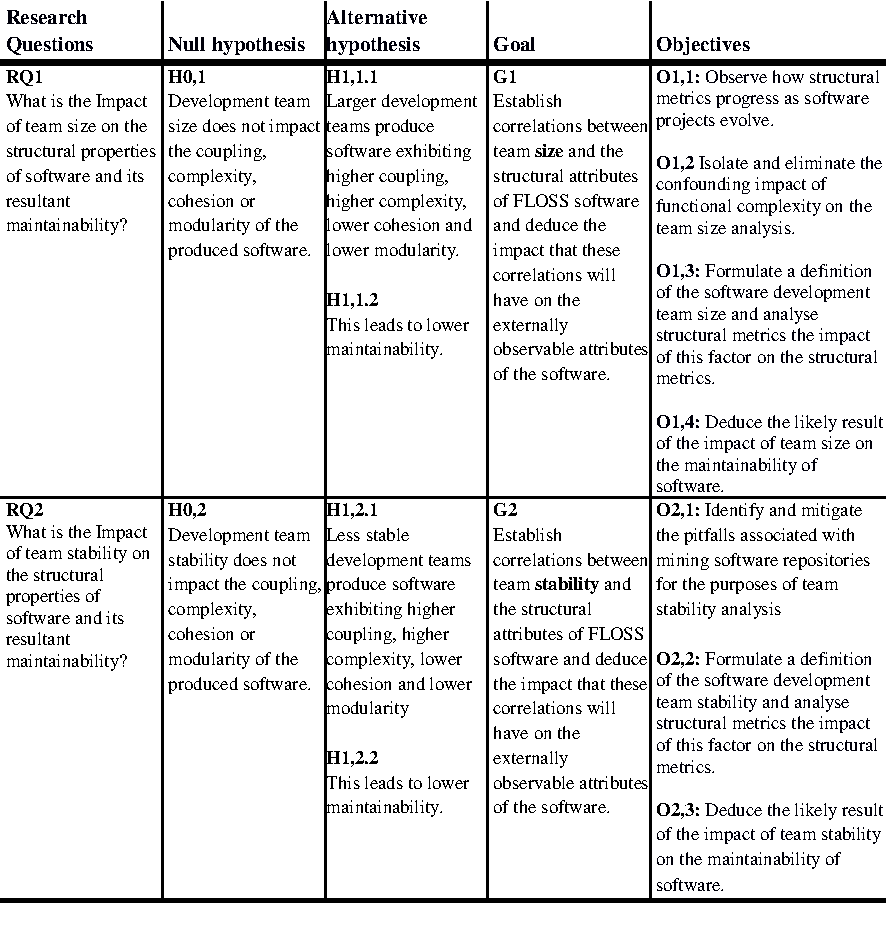
\includegraphics{ResearchSummary.pdf}
 \label{tab:researchSummary}
\end{tabular}
\end{table}

\section{Thesis Contribution} %Section - 1.7
Three main contributions to the state of the art can be identified within this thesis:

\begin{itemize}
\item \textbf{Advanced methodology to measure team size and stability:} This thesis presents an alternative approach to measuring the impact of team composition on external attributes by directly measuring the impact on its internal attributes and leveraging established research to deduce the ultimate impact on its external attributes. The impact of team size and stability on maintainability is studied through the GoogleCode forge and, in the process, numerous practical difficulties involved in mining a large and diverse forge are solved. In particular, this work identifies, quantifies and mitigates a previously undocumented and significant threat that forking can pose to the accuracy of forge network analysis.

\item \textbf{Impact of team size and stability on internal structural attributes:} A clear relationship is established between team size and stability on the internal structural attributes of software. This research concludes that those projects developed by smaller or more stable teams exhibit lower levels of coupling and inheritance complexity and higher levels of cohesion and modularity. In addition to the observed trends, the state of the art is furthered through the proposal of two new measures to capture team stability, distinguishing between stability that accumulates as a team remains unchanged across projects and the stability which accumulates through the lifespan of an individual project through the collaboration of team members. 
\item \textbf{Impact of team size and stability on maintainability of software:} Observations on the structural attributes of software will drive clear interference on the impact that team size and stability have on the maintainability of the software. By highlighting this, practitioners can measure and monitor these structural attributes allowing greater potential to mitigate the specific negative impact from the trends that are brought to light in this research.
\end{itemize}

\section{Intended Audience} %Section - 1.8
This research is intended for both the research and practitioner communities. This thesis adds an additional dimension to the existing body of research correlating internal attributes with external attributes by specifically studying the impact of team composition on internal attributes. Researchers with an interest in relating software metrics to measures of stakeholder interest will find relevance in this work. It is also intended for this work to be of value to those practitioners in the field of software development. It is the intention of this thesis to contribute towards more informed practitioner decision making around development team composition - particularly at the middle-management level. Furthermore, practically oriented observations of the impact of sub-optimal team composition, which can be monitored through static analysis of software, may find interest in the developer community.

\section{Thesis Structure} %Section - 1.10
The remainder of this thesis is arranged over six chapters, illustrated in Figure ~\ref{fig:ThesisOverview}.

\begin{landscape}
\begin{figure}[htbp!] 
\centering    
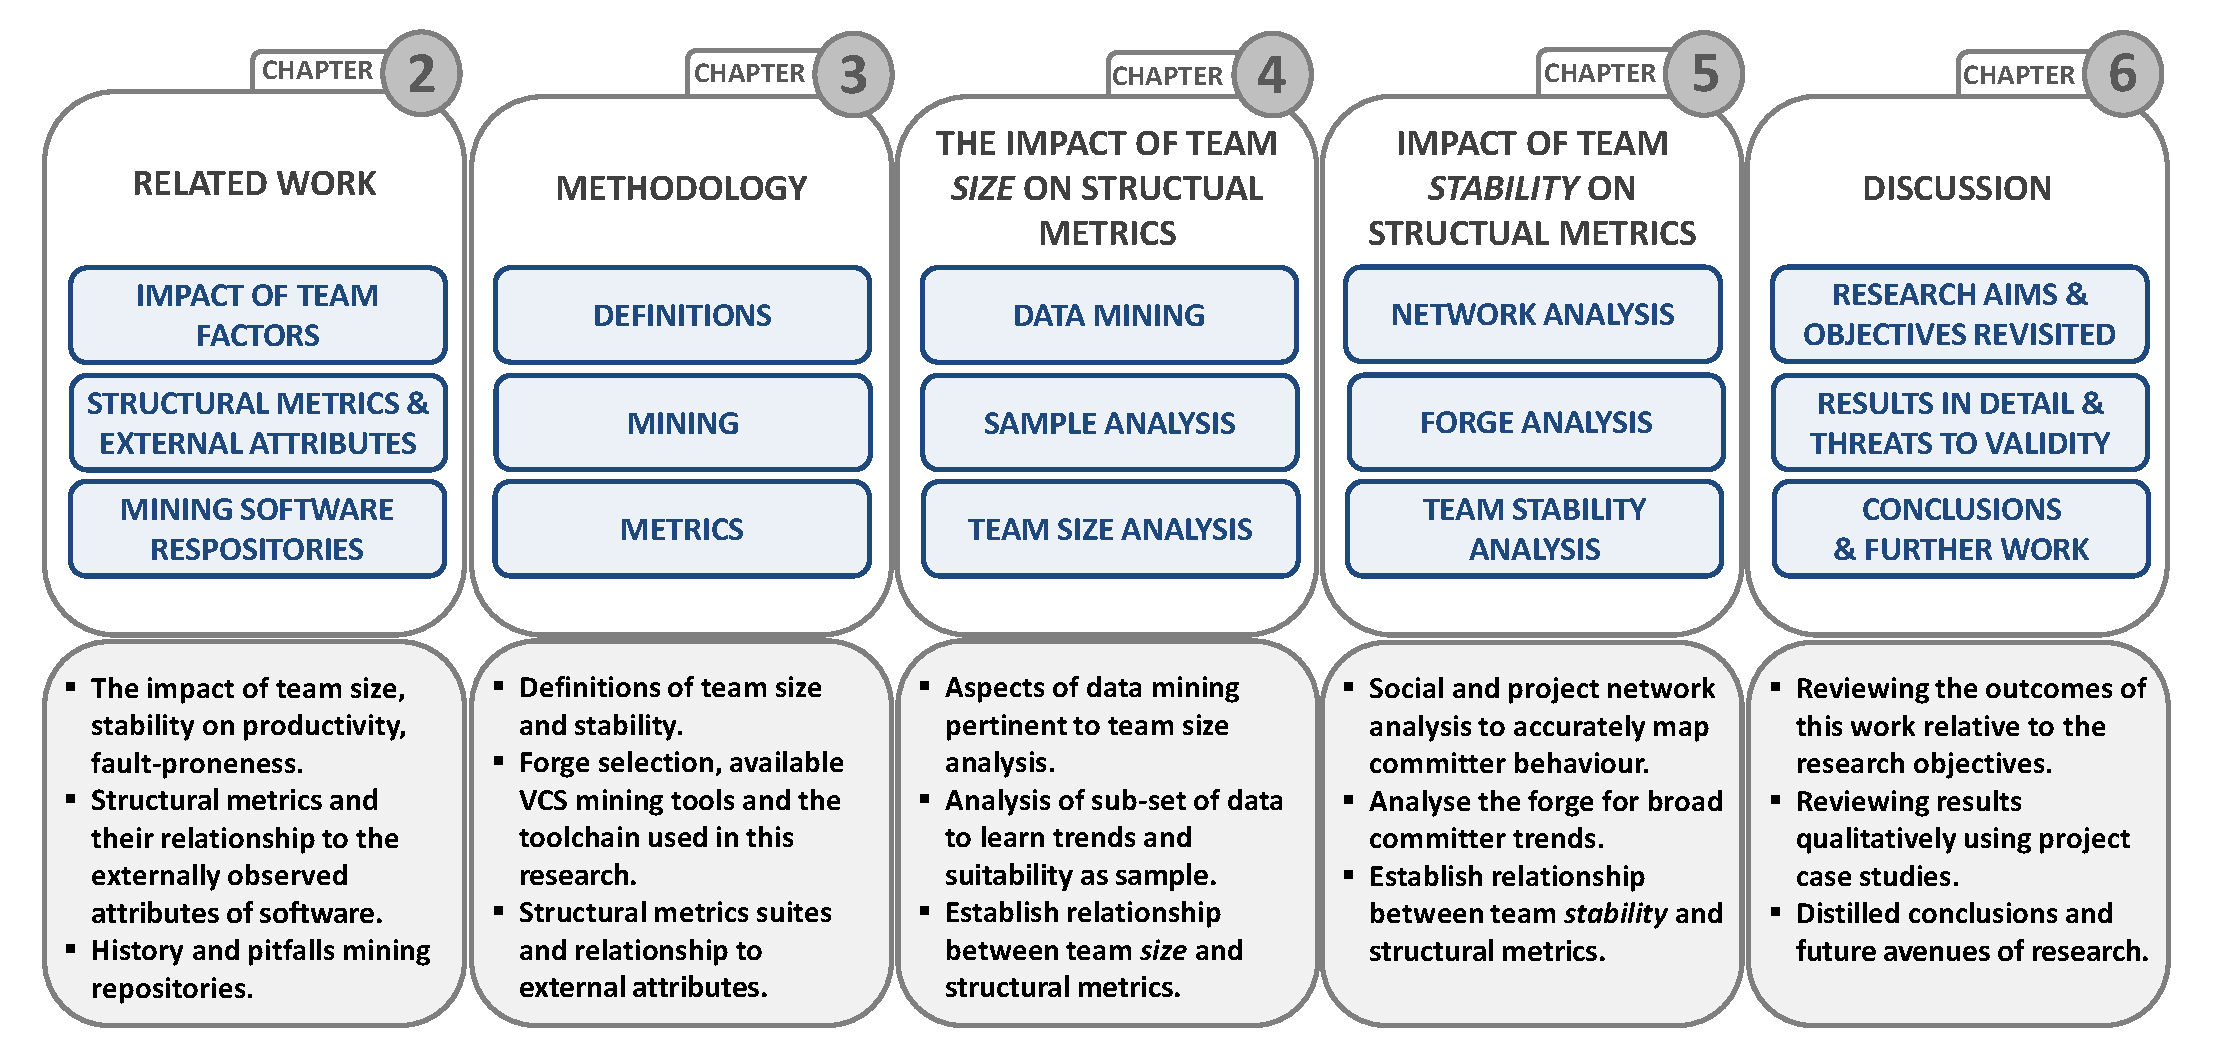
\includegraphics[width=1.4\textwidth]{ThesisOverview.pdf}
\caption[Thesis overview.]{Overview of chapter structure, colour-coded to distinguish mining from analysis.}
\label{fig:ThesisOverview}
\end{figure}
\end{landscape}
 
\textbf{Chapter 2. Related Work} Prior art is documented in three distinct fields. Firstly, a survey is conducted for previous research that establishes correlations between the development team's size and stability against attributes of stakeholder importance such as fault-proneness and team productivity. Secondly, a survey is also carried out in the established field of mining software repositories and a sampling of research that employs mining techniques to observe changes in the properties of software is discussed. Finally, software metrics are considered with a focus on structural metrics and how they are interpreted and correlated with externally observable attributes of software such as maintainability.
\newline
\newline
\textbf{Chapter 3. Methodology} In this chapter the methodological approach to this research is detailed. Existing mining tools are surveyed and the mining toolchain that underpins this research will be discussed in depth. Metrics suites are also surveyed and justification is provided for the choice of metric suite for this work. 
\newline
\newline
\textbf{Chapter 4. The Impact of Team Sizes on Structural Metrics} This chapter focuses on answering the first research question by conducting a detailed analysis on a sample of projects from the GoogleCode repository and establishing correlations between team size and the modularity, coupling, cohesion, and complexity of software.
\newline
\newline
\textbf{Chapter 5. The Impact of Team Stability on Structural Metrics} This chapter addresses the second research question with a focus on the impact of team stability accumulated through the lifespan of an individual project and across projects within a forge. To facilitate this work, network analysis is conducted across the entirety of the GoogleCode forge and, in the process, several threats to validity are identified and mitigated. The network analysis is used to identify the population of projects which is used to establish correlations between team stability and the modularity, coupling, cohesion, and complexity of software.
\newline
\newline
\textbf{Chapter 6. Discussion} The discussion chapter provides a summary of the results against the hypothesis, objectives and goals of this thesis. The results are analysed using individual projects as case studies to enable a qualitative analysis. Threats to internal and external validity and distilled conclusions are discussed. Finally, possible future avenues of research are proposed.
 
%!TEX root = ../thesis.tex

\graphicspath{{Chapter2/Figures/}{Chapter2/Tables/}{Chapter2/Charts/}}
\setlength{\parskip}{2ex}

\chapter{Related Work}

\section{Introduction} %Section - 2.1 
As outlined in the introduction, this thesis focuses on how software team size and stability impact the internal structural attributes of software. Out of this come three individual strands of related work which will be the focus of this chapter. 

The first part of this chapter reviews the studies of the impact of people factors on the externally observable attributes of software, with a focus on factors of team size and stability. This work has the greatest direct relevance to this research and is one that this thesis endeavours to further by offering an alternative approach based on the direct measurement of the internal structural attributes of software rather than the observation of external attributes. The second strand of related work in this chapter comprises the body of research that establishes correlations between the internal structural metrics of software and its external attributes. This is of crucial relevance to this work as it is that very body of research that will later be relied upon to map observable trends of structural metrics onto conclusions that have meaning from the perspective of a non-technical stakeholder with a sole interest in the external attributes of the software. The third strand of related work concerns the practicalities of mining software repositories. A survey is provided of the available tools and a summary of the pertinent challenges and pitfalls associated with mining software repositories.

\begin{figure}[htbp!] 
\centering    
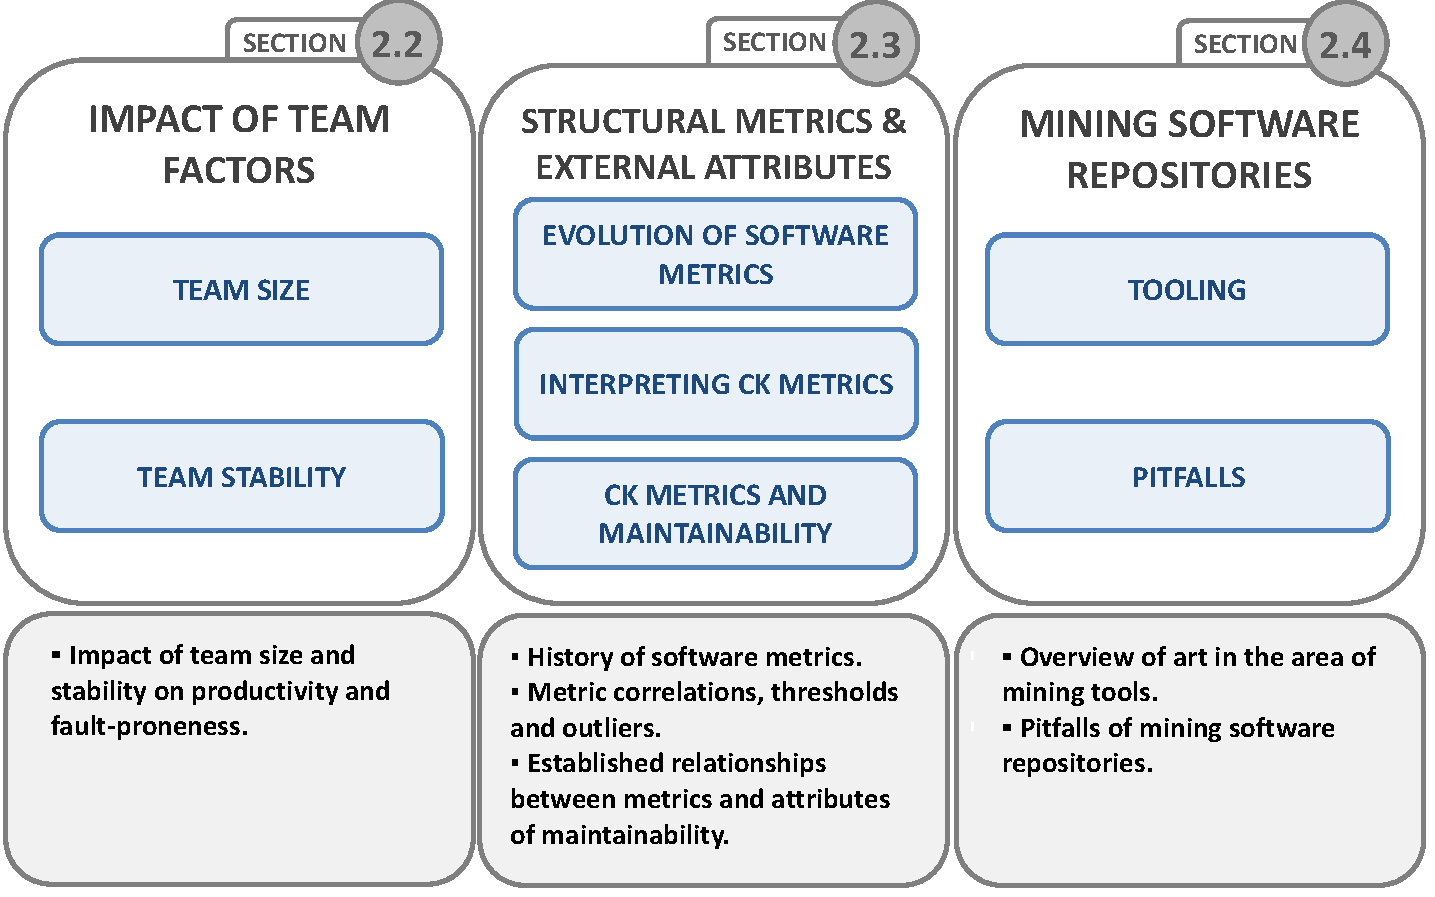
\includegraphics[width=1.0\textwidth]{ChapterOverview.pdf}
\caption{Chapter 2 outline providing an overview of the contents of each section.}
\label{fig:ChapterOverview}
\end{figure}

\section{The Impact of Team Factors} %Section - 2.2
There is a significant corpus of existing work concerned with establishing the impact of factors of team composition on the external attributes of software. This body of research models the relationship between developer and organisational factors with aspects such as fault-proneness and team productivity. This work provides the basis for the null hypotheses detailed in the previous chapter as well as the empirical approach of this study as we adopt and adapt previously established measures of team size and stability. 

\subsection{Team Size}
There have been several empirical studies investigating the relationship between development team size and the team productivity. In his popular book 'The Mythical Man Month', Brooks argues that, since software development is a complex task, the communication effort is great and adding more developers can lengthen rather than shorten the time taken to complete a task as it adds an exponentially greater number of necessary communication paths between developers \citep{brooks1986mythical} - although it is notable that Hsia et al. \citep{hsia1999brooks} argue that it won't necessarily take longer but will always increase the overall cost of delivery compared with correctly sizing the team from the outset. Roger et al., using data from 130 projects, empirically tested the impact of a number of factors on software development productivity concluding that larger team sizes significantly negatively impact software development time and productivity \citep{rodger2011knowledge}. This is corroborated in other research and using a number of empirical methods \citep{mcleod2011factors, lalsing2012people}. Scholtes et al., using a data set of FLOSS projects, perform network analysis concluding that the magnitude of the productivity decrease is related to the growth dynamics of developer coordination networks \citep{scholtes2016aristotle}. In contrast, Maillart and Sornette find that occasionally an OSS development team will exhibit 'superlinear productivity' in direct relation to the development team size, arguing that occasionally the whole is more than the sum of its parts \citep{maillart2016aristotle}.

Schweik et al. \citep{schweik2008brooks} highlight the need to inform development managers who have a stake in FLOSS projects on whether increasing the development team size is more likely to result in a successful project and help avoid 'project abandonment', arguing that this is the primary tool at their disposal to influence outcomes. Rodriguez et al., acknowledging this impact on outcomes, seeks to advise managers on the ideal team size to facilitate a process of project decomposition and distribution of work amongst appropriately sized development teams \citep{rodriguez2012empirical}. The productivity of teams sized above and below an arbitrary threshold are compared, controlling for the functional complexity of the produced software. In-line with prior literature, it is noted that those teams sized below the threshold are more productive than the larger teams. 

Pendharkar and Rodger investigated the relationship between team size and the associated cost of development \citep{pendharkar2009relationship}. They observed that the team size does not linearly increase software development cost and that, in some cases (hypothesised to be those projects suffering communication inefficiencies), larger teams require a greater than proportional increase in resources. Blackburn et al. make similar observations while also noting that greater functional complexity leads to larger teams \citep{blackburn2006brooks}. This is intuitive given that larger teams have greater knowledge and expertise and therefore would typically be deployed to more complex problems. Hericko et al. worked to define the optimal team size given these two conflicting drivers, proposing a model to minimise development effort for a given project size \citep{herivcko2008approach}.

There has also been research negatively correlating team sizes to measures used as a proxy for software quality. Nagappan used data from Microsoft's Windows Vista project to establish that metrics based on organisational structures (of which team sizes were one aspect) are a significant predictor of software fault-proneness \citep{nagappan2008influence}. Nagappan's work was later validated by Caglayan et al. who found that, while organisational metrics were out-performed by pre-release metrics such as defect counts as a predictor of ultimate fault-proneness, they were a significant predictor nonetheless \citep{caglayan2015merits}. Mockus also noted a correlation between team sizes and fault-proneness \citep{mockus2010organizational}. Bird et al. developed a more sophisticated code ownership model that distinguished between frequent 'major' committers and infrequent 'minor' committers and found that minor committers are more likely to introduce defects \citep{bird2011don}. Bell et al. observed that the number of developers that modify a file increased the probability of that file being defect prone \citep{bell2013limited}. Recently, Chopra et al. and others have moved this research forward by building prediction models to identify fault-prone classes built upon a number of predictors including team size \citep{madeyski2015process, chopra2018empirical}.

\subsection{Team stability}
Team stability (in literature also referred to as  'team familiarity' or by the antonym 'team fluidity') is also viewed as a critical success factor for an effectively functioning and performing group wherever complex problems are tackled. From cardiac surgery teams to flight crews and basketball teams, those teams that experience continuity in personnel make-up are likely to be higher performing \citep{carthey2001human, akgun2002antecedents, yeh2005influences, wiegmann2010improving, huckman2013hidden, joshi2018should}. Software development teams are no exception \citep{bao2017will}. The Scrum Agile software development methodology, for example, favours avoiding changing team members for the stated reason that stable development teams are more productive \citep{deemer2010scrum}. There is anecdotal evidence to back this claim up with practitioners reporting that fluid teams are likely to be less productive as they tend to go through the 'Tuckman cycle' (Forming, Storming, Norming, Performing) with the addition of every new team member \citep{tuckman1965developmental, linders2011establishing}.

There has been comparatively few academic studies investigating the role of team stability within the field of software development. On the empirical side, Huckman et al. conducted a detailed study of the team stability and role experience on the output of development teams \citep{huckman2009team}. Armed with a data set of over a thousand projects and defining team success criteria in terms of software defect count and adherence to deadlines and budgets,  they found that a conventional measure of experience - years of experience at a firm - was not linked with team performance. However, team stability (measured as the average number of times that each member has worked with every other member of the team) was associated with less error-proneness and more budget adherence. One stark result was that, as familiarity increased by 50\%, defects decreased by 19\%, and deviations from budget decreased by 30\%. This was confirmed by Gardner et al. who observed that teams with a high degree of team stability, captured by measuring the length of time that each team member had worked with their teammates, yielded a 10\% increase in client satisfaction \citep{gardner2012dynamically}. Mockus, studying a large commercial software project, observed that new developers were not associated with a decrease in quality (postulating that this was due to new developers being assigned peripheral tasks) while departures from the project were associated with greater fault-proneness \citep{mockus2010organizational}.
 
\section{Structural Metrics and External Attributes} %Section - 2.3

\subsection{Overview}
Underpinning the empirical approach to this research is the use of structural metrics to measure the internal attributes of software. While ISO/IEC 25010 recognises that internal quality drives external quality, it does not offer any specific direct measures for internal quality but instead offers a framework to define metrics that are influenced by internal quality. For example, maintainability is measured by the resources expended to modify software. These measures are neither direct nor predictive. Fortunately, there has been significant research in formulating such direct measures. 

Coleman et al., in the early 90s, developed a maintainability model that used static measures of source code to produce a percentage figure on how easy  a system is to support and change derived from a blend of measures including complexity metrics \citep{coleman1994using}. This metric is still used today within Visual Studio which classifies ranges which correspond to High, Moderate and Low maintainability \citep{msdn2015code}. Heitlager et al. from the Software Improvement Group (SIG) critiqued this model as presenting difficulties in re-constructing the root causes that drive a particular measure and suggested an alternative maintainability model which blends structural metrics including complexity, volume, and unit size to drive its metrics \citep{heitlager2007practical}. The strength in the SIG maintainability model is the simplicity with which a calculated index would be mapped to its constituent structural attributes.

In a similar vein, the approach of this research to observing indicators of internal quality is to directly measure the internal structural attributes of a codebase and draw upon established models to ascertain if the trends observed indicate enhanced or degraded internal software quality.

There are two primary categories of internal attributes of software - size and structure. Software size is a broad term and measurements can vary from basic line of code counts through to function-point analysis. It is tempting to assume that size is directly correlated to external attributes of fault-proneness and development effort while negatively correlated to maintainability \citep{akiyama1971example}. However, as Fenton and Bieman state, experience shows that this is not a valid assumption and that the structural attributes of software play a vital part in driving these external attributes \citep{fenton2014software}.
 
This section first discusses the metrics which can be used to capture structural attributes followed by a brief historical context. A survey of relevant software metric suites is provided alongside an overview of the research efforts to interpret metrics and modelling the impact of structural metrics on maintainability. The latter is particularly relevant as these relationships will be drawn upon later in this thesis to infer the likely impact of observations of structural metrics on the external attributes of the studied software systems.

\subsection{What Are Structural Metrics?}
Software metrics embody an empirical approach to software engineering and are primarily designed to assist in making assessments of software artefacts and development processes, in the process guiding engineers and project managers in their decision-making. A software metric is the quantitative measure of the degree to which a component, system, or process possesses a given characteristic or attribute \citep{ordonez2008state}. If used appropriately, software metrics can lead to a significant reduction in costs of the overall implementation and maintenance of the final software product. 

Structural metrics are a specific category of software metrics that allow us to measure and express the adherence of a codebase's structural attributes to sound engineering design principles. The key attributes in Object Oriented Programming are the interlinked concepts of coupling, cohesion, complexity, and modularity. These are explained as follows.

\begin{itemize}
\item \textbf{Coupling:} This is the degree to which components within software systems are interdependent. A high degree of coupling in a set of components implies that changes in one component may impact the other components in that set \citep{parnas1972criteria}. At a relatively low level, modern object-oriented languages provide paradigms (such as interfaces) to facilitate lower coupling between classes. Interfaces allow a developer to separate the method of interaction into a component from the implementation of functionality. At a higher level, enterprise design patterns such as the Service-Oriented Architecture facilitates lower levels of coupling between applications \citep{jamshidi2018microservices}. Lower levels of coupling are desirable at each level of an enterprise software system \citep{chidamber1998managerial, pressman2005software}.

\item \textbf{Cohesion:} Cohesion is a measure of the extent to which functionality within a single component belongs together. A component that exhibits a high degree of cohesiveness typically encapsulates a single set of highly related functionalities. In object-oriented languages, a high degree of cohesiveness is a desirable trait and is consistent with the 'single responsibility principle' which states that a class should have a single purpose and its functionality should be encapsulated within the class - i.e. not exposing its inner workings to other components \citep{fenton2014software}. A high degree of cohesiveness and encapsulation is associated with a low level of coupling \citep{chidamber1998managerial}.

\item \textbf{Complexity:} In the context of structural metrics, complexity refers to the structural complexity of software rather than the functional complexity. This is a contrast that will be discussed in the coming chapter in Section 4.4.3.2. Structural complexity is a measure of the degree of interactions between components in a software system \citep{fenton2014software}. A highly complex system would contain a large number of components and a large number of interactions between the components. Although the number of interactions between components is a driver of structural complexity, the nature of the interaction between two components can introduce further structural complexity if there is a dependency on the inner workings of the components (i.e. poor encapsulation and high coupling). Although functional complexity can often introduce structural complexity, all things being equal, lower measures of structural complexity are desirable.

\item \textbf{Modularity:} This refers to the extent to which a system's functionality is logically partitioned into independent components \citep{parnas1972criteria}. A high degree of modularity is desirable as it encourages low coupling and high cohesion which, in turn, reduces structural complexity \citep{parnas1972criteria, sullivan2001structure}.
\end{itemize}

\subsection{Evolution of Software Metrics}
The study and application of software metrics dates back to the mid-1960's when the primitive Lines of Code metric was routinely used as the basis for measuring software development productivity (developer LoC per month) and quality (defects per KLoC). In 1971 Akiyama proposed the use of metrics for software quality prediction proposing a regression-based model for module defect density (number of defects per line of code) where line of code was used as a crude indicator of complexity \citep{akiyama1971example}. This was one of the earliest attempts, albeit a simplistic one, to extract an objective measure of software quality through the analysis of artefacts of a system. With the increasing diversity of programming languages, it became necessary to introduce a more sophisticated model of the structural attributes of software. 

McCabe, recognizing the importance of testable and maintainable software systems, broke new ground in the area of software metrics introducing the first meaningful structural metrics \citep{mccabe1976complexity}. In 1976, motivated by the observation that half the development time is spent in testing and that most of the cost of owning a system is in its maintenance, he developed a software metric which he termed 'cyclomatic complexity'. This metric is based on a formula to calculate the number of linearly independent paths through source code. Its purpose is to identify complex software modules based on program flow. Around the same period Halstead designed a structural metrics suite based on definitions of operators and operands modelling the complexity of individual lines of code \citep{halstead1977elements}. To give a flavour of these metrics, the Halstead Difficulty uses a formula to assess the complexity based on the numbers of unique operators and operands capturing a measure of how difficult the code is to write and maintain. Halstead Effort is an estimate on the effort to rewrite a particular method.

The research community continued to be highly active in the field of structural metrics throughout the next decade \citep{cote1988software} with advances in the usage of existing 'classical' metrics \citep{behrens1983measuring, gaffney1981metrics} as well as the formulation of new structural metrics \citep{boydston1984programming, prather1984axiomatic}.

In the 90s, with the increasing adoption of Object-Oriented (OO) programming languages, the research in structural metrics took another significant step forward. Chidamber and Kemerer argued that Object-Orientation, as the most prominent advance in software development, and with yet to be established practices, necessitated measures that could guide organizations to its successful adoption. This fact, coupled with criticisms of existing metrics suites, saw the development of the Chidamber and Kemerer (CK) metrics suite, detailed in Table ~\ref{tab:ckmetricsuite} \citep{chidamber1991towards, chidamber1994metrics}. For its popularity and simplicity, as detailed later in this chapter, this is the suite that will be used to underpin the empirical work in this thesis.

\begin{table}
\captionof{table}[A summary of the CK metric suite]{A summary of the CK metric suite. For further detail on the calculations and their theoretical basis refer to the research of Chidamber and Kemerer (Chidamber and Kemerer, 1994)}
\begin{tabular}
 \centering 
 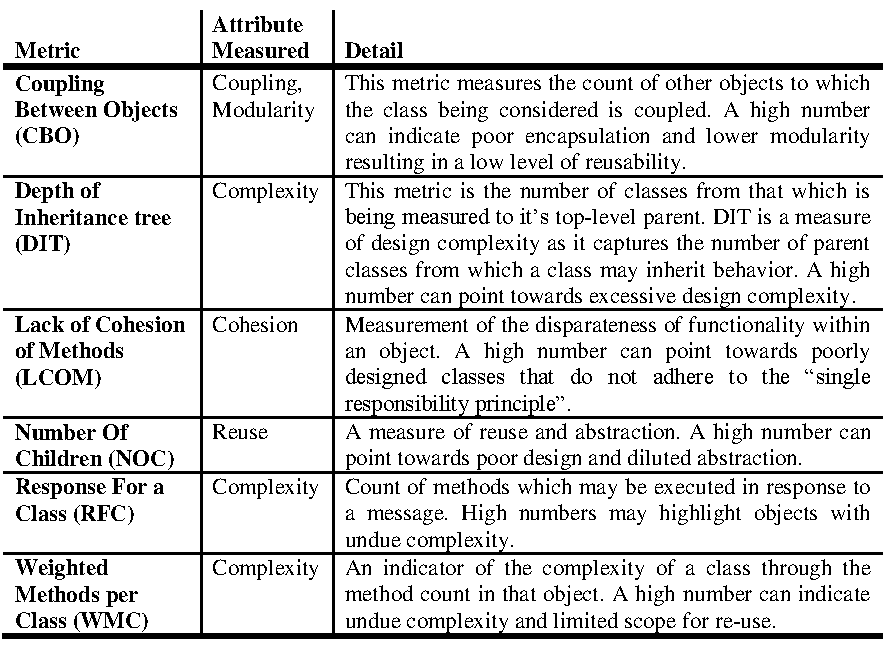
\includegraphics{CKMetricSuite.pdf}
 \label{tab:ckmetricsuite}
\end{tabular}
\end{table}

\subsection{Survey of Metrics Suites}
There are a number of structural metric suites that commonly appear in both academic literature and practitioner tools. In this section a comparative survey is provided for the most popular metric suites and justification is given to the choices in this research. The discussion is limited to object-oriented structural metrics given that, as will be discussed in the next chapter titled 'Methodology', this research studies Java software only. This is to the exclusion of suites such as the Halstead metrics. Furthermore, consideration is only given to those metric suites that comprehensively cover the key internal structural attributes - coupling, cohesion, complexity and modularity - to the exclusion of, for example, the McCabe metrics with their almost exclusive focus on structural complexity \citep{mccabe1976complexity, mccabe1989design}. For a fuller survey of the available object-oriented structural metric suites, the reader is encouraged to review the work of Gomathi and Linda Edith \citep{gomathi2013an} and Xenos et al. \citep{xenos2000object}. The survey is therefore limited to the Chidamber and Kemerer suite, the MOOD metric suite and the Lorenz and Kidd metric suite.

\begin{itemize}
\item \textbf{Chidamber and Kemerer metric suite} The Chidamber and Kemerer (CK) metric suite is one of the most cited of all structural metric suites within the academic community \citep{pressman2005software} with a great deal of research spanning the two decades since its creation. 

The CK metric suite is designed to operate on the most fundamental unit in object-oriented systems - the class. The CK metric suite contains measures that capture complexity, coupling and cohesion. The values of the measures are fairly arbitrary and there has been research into defining the thresholds that could indicate classes which would be more likely to require remedial action \citep{rosenberg1998applying}. While there has been some doubt cast on the theoretical and empirical validity of one of the measures in the suite \citep{fenton2014software}, nonetheless, this remains the most validated OO metric suite available \citep{kitchenham2010s} with a great deal of research successfully correlating the metrics to external quality attributes \citep{rosenberg1998applying, el2001prediction, basili1984software, subramanyam2003empirical}. This suite is covered in more detail later in this chapter.

\item \textbf{MOOD metric suite} The MOOD metric suite was developed by Abreu and Carapu\c{c}a in 1994 to provide system-level measures (as opposed to class-level measures) for object-oriented systems in order to guide and assess OO design quality \citep{abreu1994object}. The measures capture a broad range of structural attributes including encapsulation and polymorphism factors - factors absent from the CK metrics suite. In contrast to CK metrics where the values of the measures are arbitrary, the MOOD metric values are probabilities with values from 0 to 1 representing the likelihood of the existence of a particular attribute. Harrison et al. conducted research detailing the utility of MOOD metrics to practitioners finding that they present information that would be of general use to software managers to understand the overall attributes of a system \citep{harrison1998investigation}. MOOD metrics are not widely adopted in academic research nor industry and this is reflected in the very scarce availability of tools that generate these metrics with Project Anaylzer \citep{abounader1997data} being the only distributed tool that the author could find. This tool only had support for the Visual Basic programming language. In its favour there has been significant research analysis which largely validated the MOOD metric suite \citep{abounader1997data, harrison1998evaluation}.

\item \textbf{Lorenz and Kidd metric suite} In their book 'Object-Oriented Software Metrics' Lorenz and Kidd proposed a metric suite consisting of eleven metrics that, in a similar fashion to the CK metric suite, measured attributes at a class level \citep{lorenz1994object}. Metrics are broadly in four categories - size, inheritance, class internals (attributes that can be measured on a class in isolation such as cohesion) and class externals (attributes that capture how a class interacts with other classes such as coupling and reuse). Lorenz and Kidd also propose threshold values to help interpret metric observations. The Lorenz and Kidd suite did experience a degree of recognition in academic circles with a large number of citations \citep{nesi1998effort} but, with few validation studies \citep{sharma2012metrics} and no available tools to measure these metrics, it is fair to say that this metric suite has not experienced significant academic or practitioner adoption. This may be due to the fact that the metric suite is fairly basic and constitutes directly measurable attributes such as Number of Methods, Number of Public Variables and Number of Variables which has caused some doubt to be cast on its usefulness \citep{harrison1998investigation}.
\end{itemize}

\subsection{Interpreting CK metric values}
At a time when OO metrics were a relatively new field of study, Rosenberg proposed that metrics without interpretation guidelines are of little value. She concluded that, although some numeric thresholds were suggested by developers, there was little to justify specific values \citep{rosenberg1998applying}. She proceeded to harness experiences within the NASA Software Assurance Technology Centre (SATC) to apply a common sense approach to the formulation of interpretation guidelines of individual OO metrics including most of the CK suite. These findings are summarized in Table ~\ref{tab:rosenberg}. The table shows the objective  - the direction of trends associated with favourable outcomes - and the associated impact on the external attributes. For instance, it was concluded that developers should attempt to attain low values of LCOM (the objective), which will result in a higher degree of understandability, maintainability and reuse, while reducing development effort. 

\begin{table}
\captionof{table}{A summary of the Rosenberg OO metrics guidelines.}
\begin{tabular}
 \centering 
 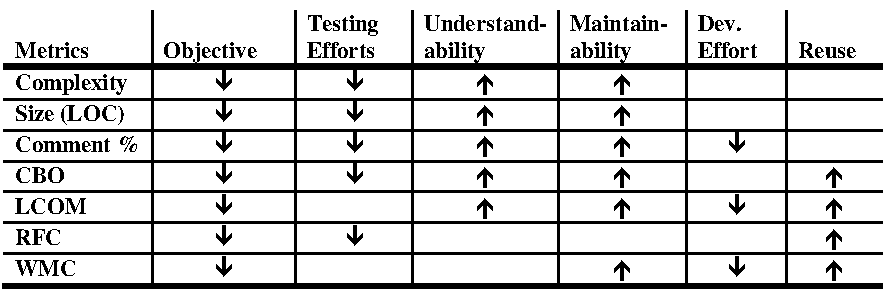
\includegraphics{Rosenberg.pdf}
 \label{tab:rosenberg}
\end{tabular}
\end{table}


However pertinent and useful, Rosenberg's research was based on the knowledge and experience within SATC, and was not an empirical treatment of software metrics. Shatnawi moved this area of metrics research forward by establishing CK metric threshold values at a number of risk levels representing probabilities of error proneness \citep{shatnawi2010quantitative}. Oliveira et al. worked to devise a technique to establish relative thresholds across a corpus of 79 projects programmed in Pharo and Smalltalk, identifying those projects that violated thresholds for a higher percentage of metric observations in order to find projects which would be expected to exhibit lower maintainability \citep{oliveira2015validating}. Hussain et al. used logistic regression to identify thresholds above which classes exhibit greater fault-proneness \citep{hussain2016detection}.

Chidamber et al. researched the question of the interpretation of the CK metric suite for managerial use and concluded that 'outlier' metric values indicate a level of complexity that would require management action \citep{chidamber1998managerial}. Chidamber et al. continued to suggest that a useful method to identify such 'outlier classes' is by applying Pareto's 80/20 principle and selecting classes which exhibit metric values from the 80th percentile for further attention - for example assigning a higher skilled developer to that implementation or assigning extra testing resources to that component.

Basili et al, motivated by the objective to leverage structural metrics to provide guidance to the areas of a system where testing efforts are best spent, established the utility of the Chidamber and Kemerer suite as a predicator of fault-prone software classes  \citep{basili1996validation}. This was achieved by assembling eight software development teams and using regression analysis to establish relationships between OO metrics and observed defects. 

These are, by no means, the only studies of this nature. Subramanyam and Krishnan conducted similar work with access to a large number of in-house developed codebases, controlling for programming language and software size, confirming the results obtained by Basili et al \citep{subramanyam2003empirical}. These results were further validated in a number of similar studies, each adding its own unique contribution \citep{el1999validation, tang1999empirical, cartwright2000empirical, el2001prediction, subramanyam2003empirical, gyimothy2005empirical, xu2008empirical, malhotra2012fault, okutan2014software, song2018comprehensive}. Table ~\ref{tab:FaultModels} surveys the empirical approach within this research.

\begin{table}
\captionof{table}{A survey of the research modelling fault-proneness as the dependent variable and CK metrics as the independent variables.}
\begin{tabular}
 \centering 
 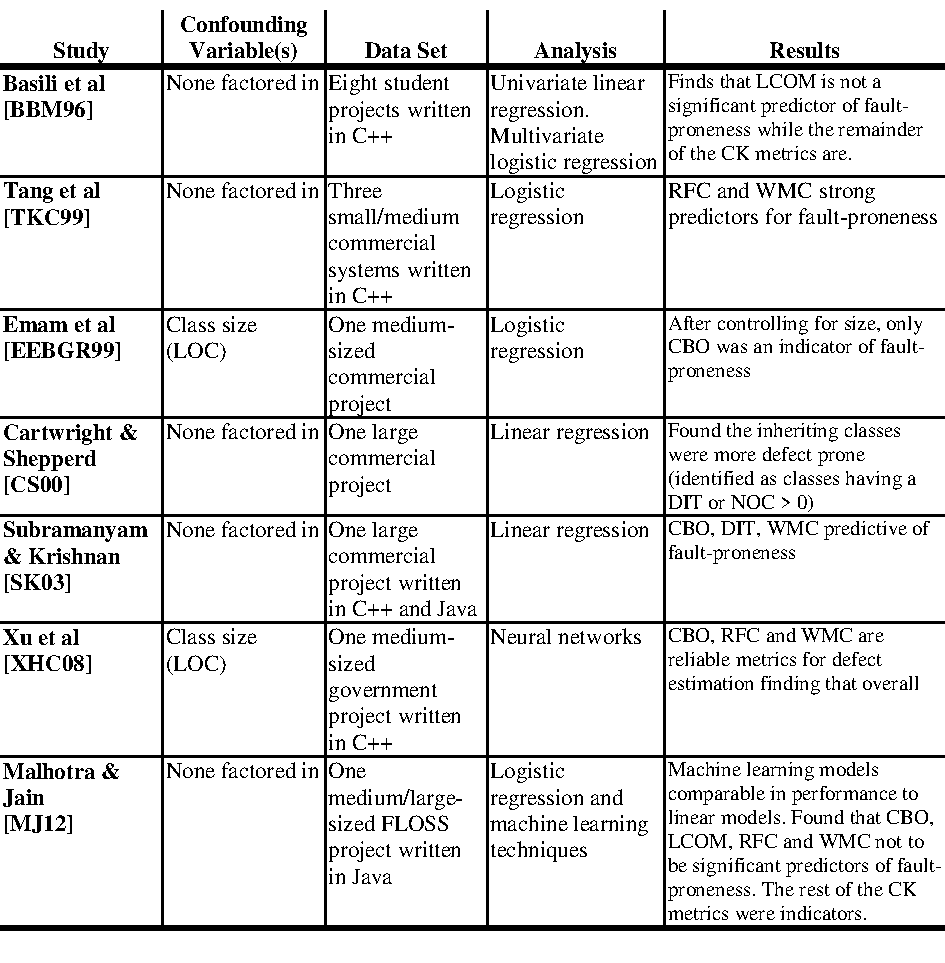
\includegraphics[width=1.0\textwidth]{FaultModels.pdf}
 \label{tab:FaultModels}
\end{tabular}
\end{table}

Saberwal et al. developed logistic regression models relating CK metrics to bad code smells driven by the desire to guide refactoring efforts to where they are most needed \citep{saberwal2013empirical}. More recently, this work was validated by Tufano et al. \citep{tufano2017and} using linear regression models. Badri et al, using similar techniques, concluded that a correlation exists between LCOM and unit test coverage, validating the use of OO metrics as a predictor of the testability of classes \citep{badri2011empirical}.

\subsection{CK metrics and Maintainability}
Santos et al and Ernst independently identified a number of issues with threshold values, foremost among them that these values make generalised statements across projects \citep{Santos2017AnES, ernst2018bayesian}. Structural metric values depend heavily on complexity and size, and therefore a single threshold value will not necessarily hold true across a diverse set of projects. Moreover, establishing a threshold across a corpus of projects using the techniques devised by Oliveira et al. is arguably of limited value to this research given the objective of establishing inferences from metric trends on how software maintainability is generally impacted by team factors. For this reason, this section focuses on surveying the research that empirically establishes a relationship between CK metric values and externally observable attributes of software in order to expand upon (and detail the empirical validation of) Rosenberg's interpretation of the relationship between CK metrics and maintainability.

As established in the previous chapter, maintainability is comprised of four sub-attributes - analysability, changeability, stability, and testability. Correia et al, through a survey-based study present the opinion of software quality experts that a number of structural attributes drive the sub-attributes of maintainability \citep{correia2009survey}, the consensus being that size, complexity, coupling, cohesion and test quality are all key factors. Chong and Lee developed a technique to visualise the structural attributes of codebases using a weighted complex network in order to capture its structural characteristics, with respect to its maintainability and reliability \citep{chong2015analyzing}. They broadly observe that high coupling and low cohesion are associated with lower maintainability, confirming the consensus of the software quality experts. Li and Henry conducted one of the first studies to determine if CK metrics could be used as a predictor of maintenance effort, concluding that DIT, LCOM, NOC, RFC and WMC all predict maintenance efforts beyond what can be predicted for size alone \citep{li1993object}.

The next section surveys research modelling the relationship between CK metrics on particular sub-attributes of maintainability and each of the sub-attributes of maintainability.

\subsection{CK metrics and the Sub-Attributes of Maintainability}
Bruntink and van Deursen used correlation analysis to study the relationship between CK metrics and the testability of software using a data set of five projects (including one open-source project) \citep{bruntink2006empirical}. Using the lines of test code and the number of test cases in the unit tests as a proxy for testability, they find that DIT, LCOM and NOC are predictors of testability. It is attributed by the authors to be due to the developers choosing not to re-test inherited behaviour from the parent class within each child class. Badri et al. furthered this research by testing a series of metrics capturing the structural attribute of cohesion for correlation (of which LCOM was one) against testability \citep{badri2011empirical}. Confirming the results of Bruntink and van Deursen, LCOM was found to be a significant predictor of testability. 

Harrison et al. used a similar statistical approach to confirm a negative correlation between WMC and the time to create automated tests for software \citep{harrison1998investigation}. 

Harrison et al. also broadened the scope of their research to cover understandability and changeability. To measure software understandability, a model formulated by Boehm et al. is used which rates software qualitatively on its structure, application clarity and self-descriptiveness \citep{boehm1978characteristics}. A simplified version of this model is replicated in Table ~\ref{tab:bohem}. Harrison et al. measure the time to implement modifications as a proxy to measuring changeability. WMC was found to be negatively correlated with understandability. Both WMC and LCOM were negatively correlated with changeability.

\begin{table}
\captionof{table}{A reproduction of Boehm's software understandability model.}
\begin{tabular}
 \centering 
 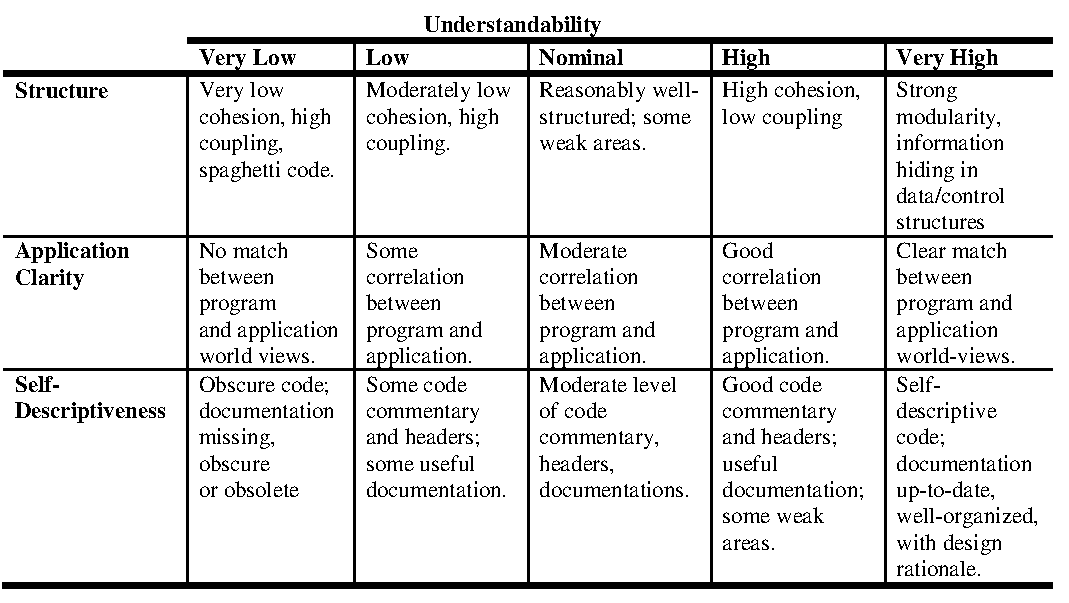
\includegraphics[width=1.0\textwidth]{BoehmUnderstandabilityModel.pdf}
 \label{tab:bohem}
\end{tabular}
\end{table}

Elish and Rine conducted a study to determine if CK metrics could be used as a predictor of the stability of software \citep{elish2003investigation}. Their research calculated the class-level stability through an algorithm that determined the likelihood that the class would be change-prone as a result of a class-level change elsewhere in the design. 

CBO, DIT, LCOM, RFC, and WMC were all found to be negatively correlated with stability. In particular CBO and RFC were strong predictors of stability. A high CBO indicates that a class depends on many other classes or that many other classes depend on it, increasing the likelihood that change ripples through to the high CBO class. Similarly, a class with a high RFC indicates a higher number of internal and external methods that may impose change on the class. 

Tables ~\ref{tab:MaintainabilitySubatrributes} and  ~\ref{tab:MaintainabilityModels} provide a summary of this survey. This will be drawn upon later in this thesis to draw insights from observations on structural metrics trends in the context of their impact on maintainability.

\begin{table}
\captionof{table}{A summary of established associations between CK metrics with the sub-attributes of maintainability.}
\begin{tabular}
\centering 
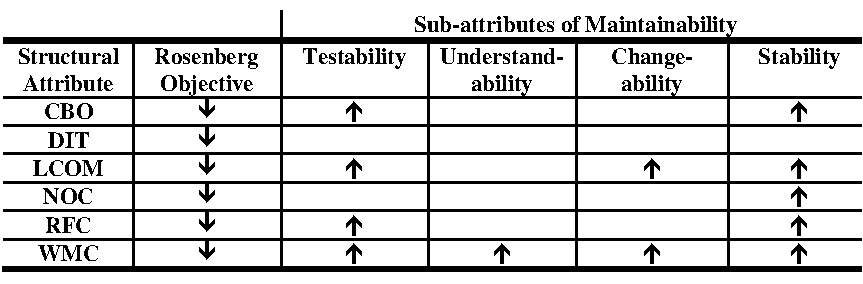
\includegraphics{MaintainabilitySubatrributes.pdf}
\label{tab:MaintainabilitySubatrributes}
\end{tabular}
\end{table}

\begin{table}
\captionof{table}{A survey of the research establishing  associations between CK metrics with the sub-attributes of maintainability. No confounding factors are controlled for.}
\begin{tabular}
\centering 
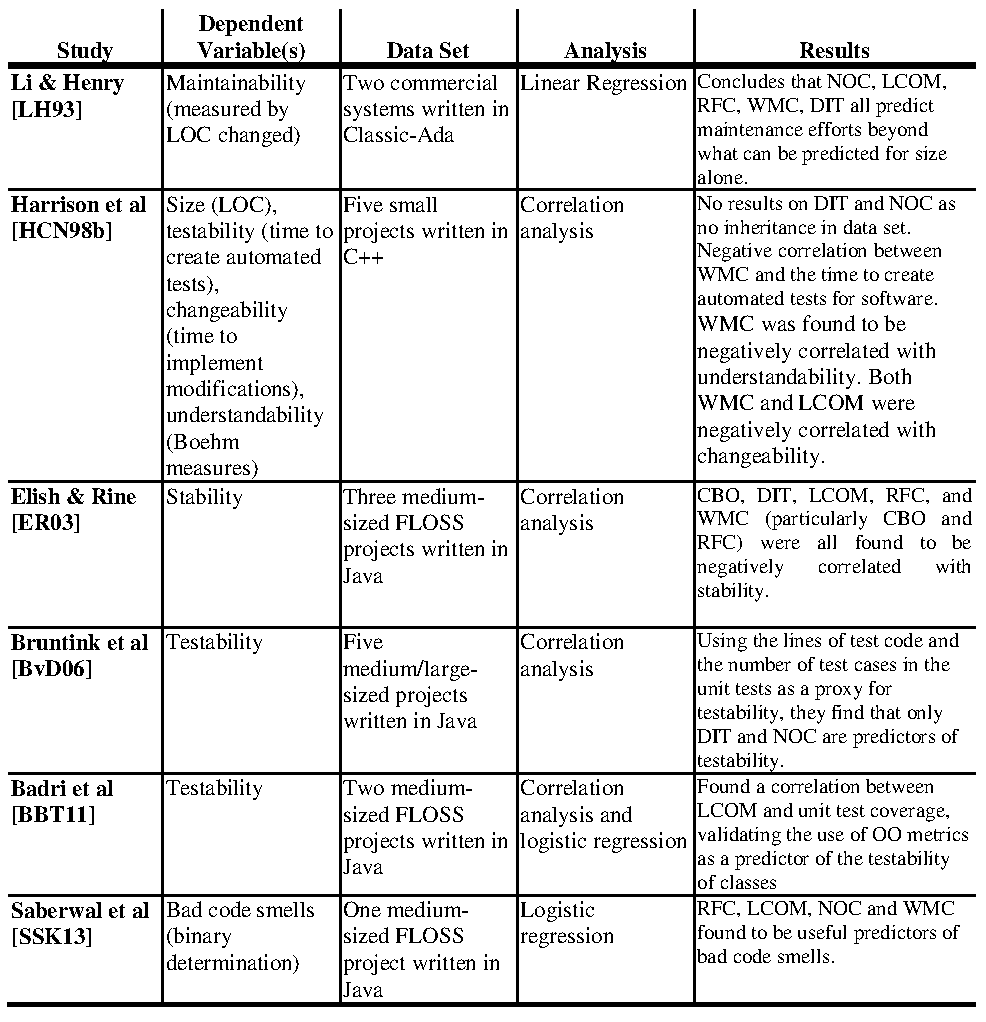
\includegraphics[width=1.0\textwidth]{MaintainabilityModels.pdf}
\label{tab:MaintainabilityModels}
\end{tabular}
\end{table}

\section{Mining Software Repositories} %Section - 2.4
Mining Software Repositories is a term that refers to the extraction, inspection, and analysis of artefacts produced through the software development process in order to deduce useful information about software projects. The intention is often to make this information available both to researchers to build upon and to industry practitioners to better inform decision-making \citep{hassan2008road}. 

This section reviews the related work in four areas. The general motivations for mining software respistories is first outlined. A survey is provided of the prior research mining and analysing forges - those centralised platforms such as SourceForge, GitHub and GoogleCode which provide the ecosystem to facilitate distributed development. Then a survey of the tools that have been developed to support the activity of mining software repositories is presented and evaluated in the context of its applicability to this research. Finally, the challenges and pitfalls associated with mining individual project repositories or entire forges are then discussed with an emphasis on aspects of network analysis and accurately determining authorship.

\subsection{Overview}
A software repository is built on a Version Control System (VCS), such as CVS \citep{cvs} or GIT \citep{git}, which is used to manage change in source code. These repositories come with a great deal of data that can be mined and subsequently analysed. Each act of file creation, deletion, or edit is represented within a 'commit'. Meta-data associated with every commit lists the paths of files that have been modified, committer details and a date. Snapshots of the source files themselves can be retrieved in their present state or at any point in their history - typically either for manual qualitative analysis or more often by machine-driven quantitative analysis. By mining software repositories, the evolution of software can be observed. 

 Researchers typically inspect particular characteristics of a system throughout its evolution and observe trends and relationships. Kagdi et al. classify these types of studies into one of two categories \citep{kagdi2007survey}. The first category of investigations observes the changes in properties through multiple versions of a system - for example, defect density or software complexity \citep{yamashita2017software, agrawal2018we, tian2018statistical}. The second category of investigation is more interested in the mechanics of the changes in artefacts - for example who is revising source files, how often, and the drivers of change \citep{lee2017understanding, ortu2018mining}. This research is focused on mining software repositories to study changes in properties.

Studying aspects of software engineering, and indeed social science, through the mining and subsequent analysis of data from FLOSS repositories is a well-trodden path with a large volume of academic studies leveraging this approach \citep{hassan2008road, hemmati2013msr}. There are a number of reasons why this approach is widely adopted:

\begin{itemize}
\item \textbf{Depth:} There are several million FLOSS projects available in the public domain - with thousands being added on a daily basis. Although a large number of projects never reach maturity \citep{comino2005planning}, this is still an extremely rich resource to mine \citep{deshpande2008total}.
\item \textbf{Access:} Under the GNU license under which FLOSS projects are typically distributed, no restrictions apply to extracting, analysing, and publishing data derived from the publicly available source code or associated meta-data \citep{license2007version}. In contrast, access to source code for proprietary commercial software is often restricted to the relevant in-house development team only for security, compliance and competitive reasons.
\item \textbf{Rich data:} Open-source forges such GitHub \citep{github} or GoogleCode \citep{googlecode} come with a great deal of data that can be mined and analysed. In addition to the VCS commit data, there is also project level information that is made available including project categorisation, activity, artefacts, and bug reports. The FlossMole project was established to extract, normalise and publish project-level meta-data available across forges in unified format \citep{howison2009flossmole}. Some of their artefacts are used in this research.
\end{itemize}

\subsection{Forges}
There have been a number of studies where a multitude of repositories have been mined within a broader forge. These studies have typically focused on analysing project artefacts to study the impact of developers, the forge, or to otherwise facilitate the process of FLOSS adoption.

Eilhard and M{\'e}ni{\`e}re conducted an empirical study of 10,533 projects on SourceForge assessing the productivity of development team members, finding that volunteers tend to score lower than corporate developers \citep{eilhard2009look}. Similarly corporate developers are found to benefit more from 'knowledge spillover' - the positive exchange of information between individuals within an organisation. Capiluppi and Beecher carried out a comparative analysis between two large forges - Debian and SourceForge - to assess whether the decay of software architecture is impacted by the forge \citep{capiluppi2009structural}. While Debian was found to host more complex projects, it also exhibited greater 'anti-regressive' work to reduce this complexity over time. Capiluppi et al. also attempted to identify whether the forge could have an impact on the structural metrics of the developed software \citep{capiluppi2009quality}. They find no significant difference between metrics on the KDE forge (which specifically reinforces coding standards) compared with SourceForge (which does not do so). 

Bagnato et al. state that assessing if a FLOSS project meets the requisite standards for business adoption is a non-trivial task and requires analysis of multiple project artefacts including source code, documentation and issue trackers \citep{bagnato2017developer}. To support this process, they developed an IDE plug-in called CrossMiner which extracts information from these various data sources for a given project and presents it within a single screen. In a similar vein, Wasserman et al. developed a methodology and a tool to assess the 'business suitability' of FLOSS projects by, again, mining these data sources and rating projects on a series of criteria including  functionality, documentation and adoption \citep{wasserman2017osspal}. More recently Tamburri et al., also motivated by the need to provide greater rigour around the process of FLOSS adoption developed a tool called 'Yoshi' to analyse the open-source community and categorise it into one of a number of known organisational patterns \citep{tamburri2018discovering}. Applying their analysis to 25 projects from GitHub, they assert that they find value in measuring and monitoring these key organisational aspects. 

\subsection{Mining Tools}
With the advent of open-source repositories, researchers acquired access to an large and rich data set. This led to an improvement in the tooling used to mine repositories. German \citep{german2004mining} documented the challenges involved in mining the CVS repositories of the GNOME project. German et al. \citep{german2005framework} followed this up with a review of some tools the mine repositories and suggested a comparison framework to support this activity. The available tools were generally found to be disparate and fulfil the relatively narrow requirements of the research groups that developed them. More recently Tiwari et al. proposed an 'app store' model for packaging and distributing software repository mining tools utilising their platform 'Candoia' \citep{tiwari2017candoia}. While this platform has not seen significant adoption, the concept is undoubtedly a step forward. In the next chapter a review is provided of the tools of direct relevance to this work and the potential for employing these tools is evaluated in the context of the data extraction and analysis requirements of this research. 

\subsection{Pitfalls}
As will be discussed during the course of this thesis, when mining a significant amount of repository data, there are a number of pitfalls that, where ignored, can constitute a serious threat to the validity of the research. This is an interesting stream of research in its own right and there are a number of studies that typically focus on either a particular VCS or particular challenges that exist across VCS. This is covered  in the next sub-section titled 'Data Extraction and Entity Reconciliation'. Through the course of this research the pitfalls around conducting analysis in a forge containing forked projects has been a particularly significant challenge and will emerge as dominant theme later in this thesis. Prior research in this area is documented in the sub-section titled 'Forking and Cloning'.

\newline
\textbf{2.4.3.1 Data Extraction and Entity Reconciliation}
\newline
German did some early work in the field of mining software repositories and raised practical concerns with the volumes of data involved in mining a single significant CVS repository, proposing a graphical tool to help visualise large data sets (eventually becoming the SoftChange tool) \citep{german2004mining}. Bird et al. conducted a similar study against the GIT version control system bringing out some its particular idiosyncrasies, particularly around the pervasive nature of branch development and the implications that this has on how to interpret revision history \citep{bird2009promises}.

Also relevant to this work is the research that focuses on the pitfalls associated with mining data from forges. Iqbal et al., attempting to solve for the challenge of integrating data across multiple FLOSS code forges propose the use of so-called 'semantic web' technologies to represent the meta-data contained therein \citep{iqbal2012integrating}. They argue that linking the various developer aliases across forges can produce a holistic picture of their activity, unlocking in the process some useful analytics. To do so they propose an email similarity algorithm which is not fundamentally dissimilar to that used within this research and described in Section 5.2.1 \citep{iqbal2015large}. Goeminne and Mens also highlight the challenges in reliably establishing committer identities across repositories, conducting a survey of a variety of algorithms available to help mitigate this \citep{goeminne2013comparison}. Their work was built upon by Xiong et al. who employed Natural Language Processing to perform identity reconciliation across GitHub and Stackoverflow, the popular developer community-based knowledge base \citep{xiong2017mining, github, stackoverflow}. In a similar vein, Squire tackled the specific problem of identifying projects that reoccur across forges and presented a method to score similarity between project pairs \citep{squire2009integrating}.

Howison and Crowston documented the promises and perils of mining SourceForge, documenting the practical challenges of data extraction, data analysis and research design \citep{howison2004perils}. More recently Kalliamvakou et al. conducted a similar study against GitHub finding that many projects were inactive or have very few commits and most repositories were for individual development \citep{kalliamvakou2014promises}. Some of their work informs the forge and repository analysis documented in Chapters 3 and 4 in an effort to understand the extent that the trends observed in SourceForge and GitHub apply to the forge that is the subject of this thesis: GoogleCode.

\newline
\textbf{2.4.3.2 Forking and Cloning}
\newline
Forking refers to the process of creating an alternate and independent software development stream from an existing project, often retaining the original VCS revision history of the parent. When mining data from projects within open-source forges it is crucial to reliably establish the unique commit activity on a given project and the fact that the forking process duplicates the revision history across multiple projects introduces an avenue of potential distortion to the raw results. When conducting committer collaboration analysis, it is essential that each committer's contribution is accurately and reliably identified without threat of misreporting child project engagement when there was only engagement in the parent project. This is particularly true in the case of this research where a particular form team stability is measured by observing the number of previous projects that committers have partnered in. This will be covered in greater detail in Chapter 5.

Nyman and Mikkonen conducted research to establish the most common motivations for forking within SourceForge \citep{nyman2011fork}. The methodology to identify forked projects was to execute a keyword search within project descriptions to find references to forking. Although this approach suffices when attempting to locate a statistically significant  sample to study, relying on developers to specifically declare a project as 'forked' in the description does not help us identify the full set of forked projects.

Robles et al. \citep{robles2006mining} suggested a fairly manual approach for locating significant software forks that involved searching Wikipedia using the term 'software fork' and manually navigating to the project homepage to extract key information ahead of a study on the motivations and outcomes of forking. This is an adequate approach when attempting to extract a sample of forked projects for further study but cannot be applied to the large-scale mining of software forks within open-source forges. More recently, Jiang et al conducted similar research against the GitHub forge and they were able to directly use project meta-data made available by the forge (a recent innovation) to identify forks \citep{jiang2017and}.

As part of the process of maintaining a forked project, it is often desirable or indeed necessary to import changes from the master project. Ray et al. developed a tool called REPERTOIRE to automate the identification of common commits between known forked projects through comparison of source files but it does not attempt to identify forked projects in a wider open-source forge \citep{ray2012repertoire}. This is the most sophisticated approach to detecting forks that is noted in the prior literature. In this general research field there have also been a number of efforts to automate the identification of 'cloned code' i.e. source code that is duplicated within a single project or across projects within a forge. This field of research has drawn some attention due to the potential negative impact that code cloning has on maintainability \citep{lozano2007evaluating}. Lozano and Wermelinger developed a prototype tool called 'CloneTracker' and applied it to the study of changeability within software containing clones \citep{lozano2008assessing}. Clones within a wider forge could indicate the presence of forking, making it valuable input for a heuristic that identifies such projects. Gharehyazie et al. developed a tool called Clone Huntress which identifies code clones in GitHub with the motivation of simplifying 'code foraging' - the process of discovering code within a broader repository that may be of relevance to the 'forager' \citep{gharehyazie2018cross}.

Schwarz et al. \citep{schwarz2012often} developed a set of lightweight techniques based on hashing algorithms to identify cloned code in a way that, in theory, could  scale up to an entire forge. Lee et al. \citep{lee2010instant} developed similar techniques to support instant cloned code researches (albeit designed to work within a single repository only) based on a more sophisticated multi-dimensional indexing algorithm. This is a particularly active research area with recent efforts to identify code clones using an array of novel techniques including image processing and machine learning \citep{ghofrani2017conceptual, ragkhitwetsagul2018picture}.

This research builds upon earlier work by developing a framework that employs heuristics, including mining version control histories and project meta-data with the objective of identifying forks to enable accurate analysis across a large forge.

\section{Chapter Review} %Section - 2.5
This chapter provided a literature review in three fields that are directly related to this thesis. First, the impact of the development team�s size and stability on key project attributes was considered. The work of Nagappan et al., Mockus, and Caglayan et al. was discussed, finding a correlation between team size and fault-proneness \citep{nagappan2008influence, mockus2010organizational, caglayan2015merits}. Similarly, the research of Huckman et al. and Gardner et al. was covered, establishing a relationship between team stability and fault-proneness as well as overall client satisfaction \citep{huckman2009team, gardner2012dynamically}. The second strand of research that was discussed was the impact of CK metrics on the external attributes of software, particularly the sub-attributes of maintainability; testability, stability, changeability, and stability. Tables ~\ref{tab:FaultModels} and ~\ref{tab:MaintainabilityModels} documented the empirical approaches to the prior research along with the key findings. Finally, this chapter provided a review of most relevant research in the field of mining software repositories focusing on FLOSS forges previously mined and the pitfalls associated with these mining efforts.

The next chapter covers the methodological approach to this research covering team size and stability definitions, the forge mining toolchain, and the process of selecting a metrics suite, crucial to the empirical measurement of structural attributes.
%!TEX root = ../thesis.tex

\graphicspath{{Chapter3/Figures/}{Chapter3/Tables/}{Chapter3/Charts/}}

\chapter{Methodology}

\section{Introduction} %Section - 3.1 

This chapter is divided into three sub-sections documenting the methodological approach to each of the key challenges in observing the impact of team factors through mining software repositories. As reflected in Figure ~\ref{fig:chapteroverview} outlining the structure of this chapter, these challenges are broadly in the categories of Definitions, Mining and Metrics. In order to begin to model the relationship between team factors and the internal attributes of FLOSS software, it is first necessary to define team size and stability and establish an empirical approach to their measurement. This is the topic of the first section in this chapter. The second section is concerned with the identification of an appropriately rich data set to study which, fortunately, open-source repositories provide with few technical limitations. The criteria of selecting a forge to mine will be articulated and a mechanism to mine this data and extract information in a consistent, reliable and repeatable way is described. In its final section, this chapter details the approach to measuring the pertinent internal structural attributes of the code through the evolution of the project. 
 
\begin{landscape}
\begin{figure}[htbp!] 
\centering    
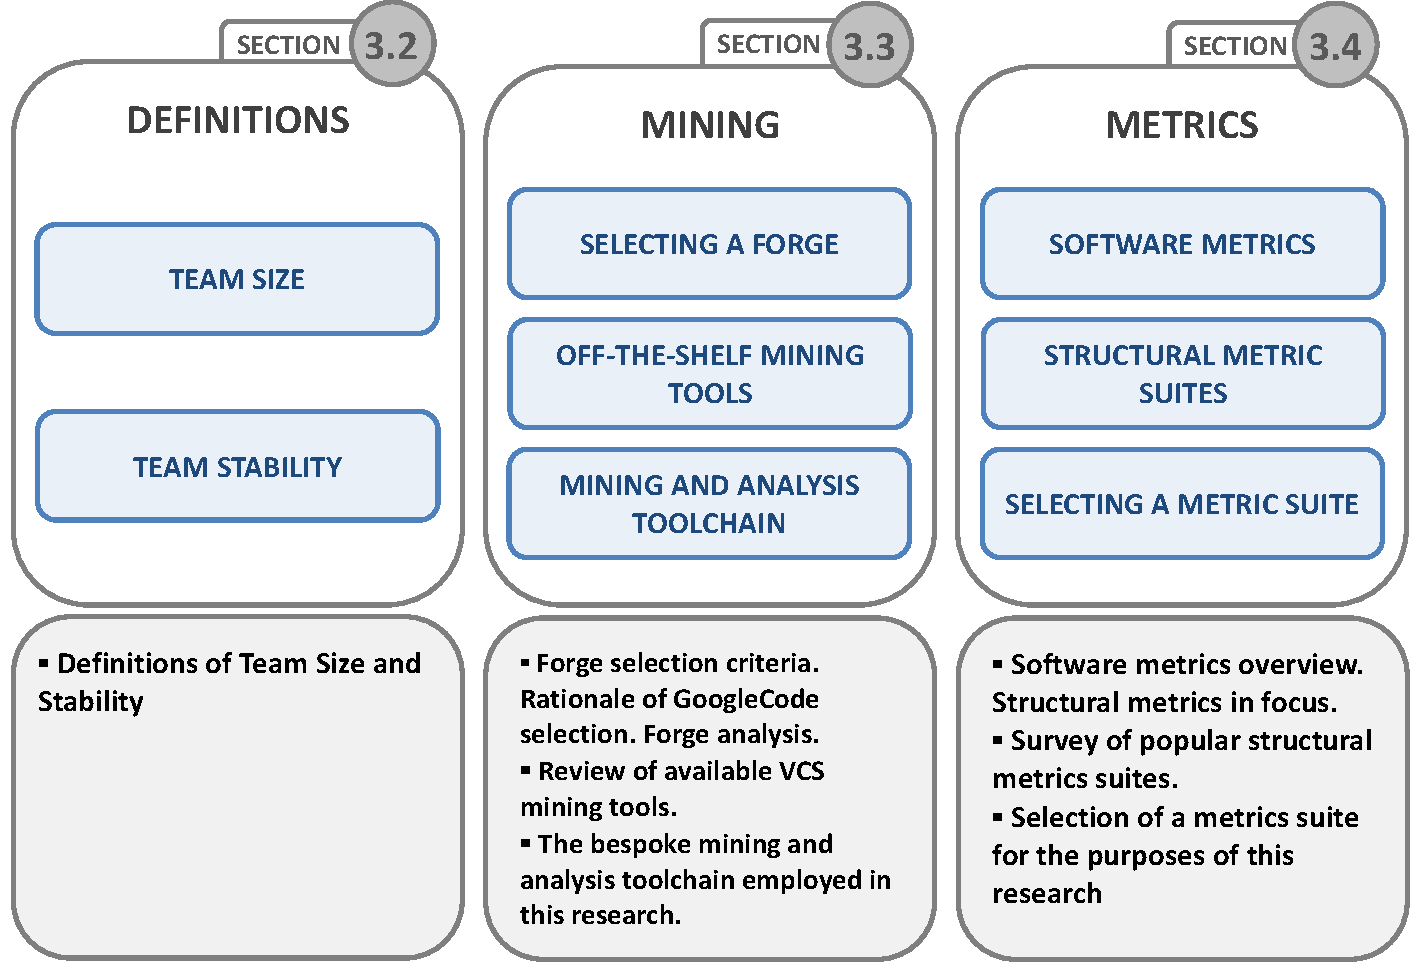
\includegraphics[width=1.1\textwidth]{ChapterOverview.pdf}
\caption{Chapter 3 outline providing an overview of the contents of each section.}
\label{fig:chapteroverview}
\end{figure}
\end{landscape}

\section{Definitions} %Section - 3.2
\subsection{Development team size}
There are a number of possible definitions of a software development team. Both Capra and Wasserman and Smith et al. consider a team to consist of all developers to have worked on a codebase for any length of time \citep{smith2001empirical, capra2008framework} while Nagappan et al. \citep{nagappan2008influence} consider the development team to also include management, administration and operations personnel. Given the context of mining open-source repositories, there is a preference to define team size as the cumulative total of all unique committers present in the revision history in the version control system of a given project. This is the definition that is adopted by this research as it is consistent with the prior literature, simple to measure and reproduce, and elegantly enables the representation of the plurality of the unique development design approaches that may have influenced the evolution of a codebase. Independently, Rempel and Mader developed the same approach to measuring development team size through their work studying quality factors in FLOSS repositories \citep{rempel2017preventing}.

There are some potential limitations to this approach, most notably that we do not distinguish between frequent committers and causal (infrequent) committers. As will be discussed later in this thesis, while it is true that the majority of commit activity takes place by a minority of committers, nonetheless the majority of committers do make a significant contribution and cannot be discounted, hence this is not regarded as a threat to validity. Similarly, when defining the team, the time during which developers contributed to the project is not considered. While it could be considered counter-intuitive that developers making contributions without any time overlap be considered part of a single team, analysis of the data sample shows that this is by far the exception in the GoogleCode forge, with the vast majority of developers making contributions in overlapping time windows with their fellow team members.

\subsection{Development team stability}
There has been relatively little empirical work that investigates the stability of development teams and its impact on aspects of the software development process. This could be due to the fact that it is a non-trivial task to capture a measure of stability. In the prior literature, team stability is also referred to using the terms team fluidity or team familiarity \citep{huckman2009team} and care is taken to distinguish this concept from 'team tenure'- i.e. the cumulative programming experience of the individuals on the team \citep{hackman2002leading}. To measure team stability a similar approach to Huckman et al. \citep{huckman2009team} is adopted, defining this as the cumulative time that each member has worked with every other member of the team. This approach is consistent with the limited prior research in this field and offers a simple, easily understood measure. Chapter 5 expands on this definition and proposes a methodology to calculate stability as it accrues within a project team.
	
\section{Mining} %Section - 3.3
\subsection{Overview}
Mining Software Repositories is a term that refers to the extraction, inspection, and analysis of artefacts produced through the software development process in order to deduce useful information about software projects. The intention is often to make this information available both to researchers to build upon and to industry practitioners to better inform decision-making \citep{hassan2008road}.

A software repository is built on a Version Control System (VCS), such as CVS \citep{cvs} or GIT \citep{git}, which is used to manage change in source code. These repositories come with a great deal of data that can be mined and subsequently analysed. Each act of file creation, deletion, or edit is represented within a 'commit'. Meta-data associated with every commit lists the paths of files that have been modified, committer details and a date. Snapshots of the source files themselves can be retrieved in their present state or at any point in their history - typically either for manual qualitative analysis or more often by machine-driven quantitative analysis. By mining software repositories, the evolution of software can be observed. 

Studying aspects of software engineering, and indeed social science, through the mining and subsequent analysis of data from FLOSS repositories is a well-trodden path with a large volume of academic studies leveraging this approach \citep{hassan2008road, hemmati2013msr}. There are a number of reasons why this approach is widely adopted:

\begin{itemize}
\item \textbf{Depth:} There are several million FLOSS projects available in the public domain - with thousands being added on a daily basis. Although a large number of projects never reach maturity \citep{comino2005planning}, this is still an extremely rich resource to mine \citep{deshpande2008total}.
\item \textbf{Access:} Under the GNU license under which FLOSS projects are typically distributed, no restrictions apply to extracting, analysing, and publishing data derived from the publicly available source code or associated meta-data \citep{license2007version}. In contrast, access to source code for proprietary commercial software is often restricted to the relevant in-house development team only for security, compliance and competitive reasons.
\item \textbf{Rich data:} Open-source forges such GitHub \citep{github} or GoogleCode \citep{googlecode} come with a great deal of data that can be mined and analysed. In addition to the VCS commit data, there is also project level information that is made available including project categorisation, activity, artefacts, and bug reports. The FlossMole project was established to extract, normalise and publish project-level meta-data available across forges in unified format \citep{howison2009flossmole}. Some of their artefacts are used in this research.
\end{itemize}

\subsection{Selecting a forge to mine}
There are a number of popular open-source project hosts or 'forges'. According to research in 2011 (at the outset of this research's data collation activities) in terms of the number of commits, GITHub was the most popular, followed by SourceForge and then GoogleCode \citep{grady2011what}. Each of these forges attracts has a unique and varied make-up of languages making up its project population - see Table ~\ref{tab:LanguagePopularity}.

\begin{table}
\centering 
\captionof{table}{Popularity of languages in top 3 open-source software forges (reproduced from Redmonk \citep{grady2011what})}
\begin{tabular}
 \centering 
 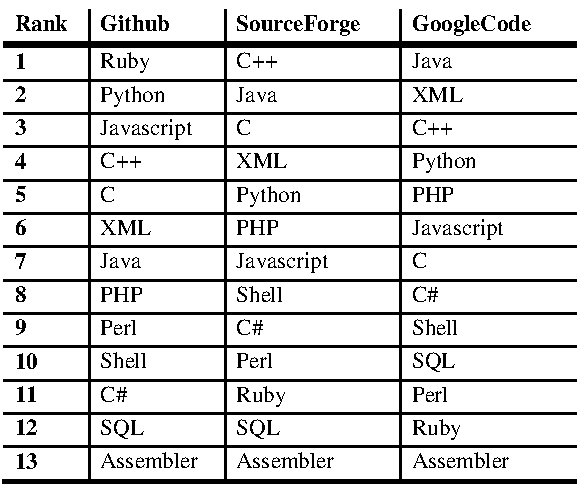
\includegraphics{LanguagePopularity.pdf}
 \label{tab:LanguagePopularity}
\end{tabular}
\end{table}


The practicalities of constructing a toolchain that is capable of mining data from a VCS and subsequently conducting static code analysis to extract the pertinent internal attributes of the software meant that it was going to require significant additional effort to accommodate more than one programming language. Given that one of the aims of this work is to maintain the relevance of this work to both the research and practitioner communities, it was logical to select a programming language with a high degree of popularity. For this reason, the Java was chosen as it consistently rates as the programming language with the highest adoption rates \citep{tiobe2017}. This also has the fortunate consequence of meaning that in most large forges there are a large number of Java projects available for study.  Furthermore, from a static code analysis tooling perspective, Java is very well supported.

GoogleCode was the open-source forge selected for its popularity and high level of Java adoption rates. Another strong advantage in favour of GoogleCode was that they allowed project administrators to choose from among three available version control systems - Subversion, GIT, and Mercurial - on which to host their source code meaning that the mining toolchain would be sophisticated enough for others to reuse to mine GitHub (which uses GIT as its underlying VCS) or SourceForge (which uses Subversion and Mercurial). This is helpful as it means that the toolchain developed for this research can have utility across a broad set of forges. This is particularly pertinent given that GoogleCode announced that it was shutting down their service and entering 'archival mode' - meaning that any future research on active projects will not happen on the GoogleCode forge. 

At this point it is also worth noting that, since the selection of the repository to study, the landscape has significantly changed and new repositories such as Assembla \citep{assembla}, and Gitlab \citep{gitlab} have established a strong presence - both of which use GIT as the underlying VCS - helpfully ensuring that the toolchain remains current.

\subsection{Overview of the GoogleCode forge}
As of May 2012, GoogleCode hosted 236,787 projects of which a significant number has seen sustained developer activity. GoogleCode projects are assigned 'labels' by the project administrators to assist in categorising the project. Many projects are 'forks' from popular projects - often where developers choose to take the project evolution in a slightly different direction or choose to 'experiment' on the codebase in their own sandbox. Forked projects retain the revision history of the original project which creates a challenge in ensuring that a forked project with a handful of commits isn't mistaken for the more popular parent project. As this is a particularly difficult challenge for which a unique solution was devised, a section is devoted to this topic later in this chapter.

The GoogleCode repository was started on the 27th of July 2006 \citep{shankland2006google} and the decision was announced nine years after its inception for its shut down \citep{dibona2006bidding}. This offers a unique opportunity to observe a forge throughout its lifespan. As we study commit patterns, it is notable in Figure ~\ref{fig:HistoricGoogleCodeActivityLevels} that the cumulative number of commits across all projects grows from the low hundreds at the forge initiation to a peak of over 10K commits per day. It is also notable that the committer activity begins to steadily tail off towards the end of 2010 as projects migrate to more popular repositories such as GitHub. In the first half of 2011 the commit activity on GitHub surpassed GoogleCode, SourceForge and Microsoft Codeplex combined \citep{redmonk2011}. This shift led industry commentators to observe that in 2011 GitHub had become the major centre of gravity within the open-source space. This is likely attributable to the collaborative nature of its offering which pushed the boundaries of 'social coding' by providing transparency on contributors activity and allowing them further their skills and manage their reputation \citep{dabbish2012social}. As GitHub continued its exponential growth over the subsequent years, GoogleCode did not compete in a meaningful way by enhancing or rebooting its offering. In this context, it is easy to rationalise Google's decision to shut down the repository, closing the forge to new project creation in 2015.
 
\begin{figure}[htbp!] 
\centering    
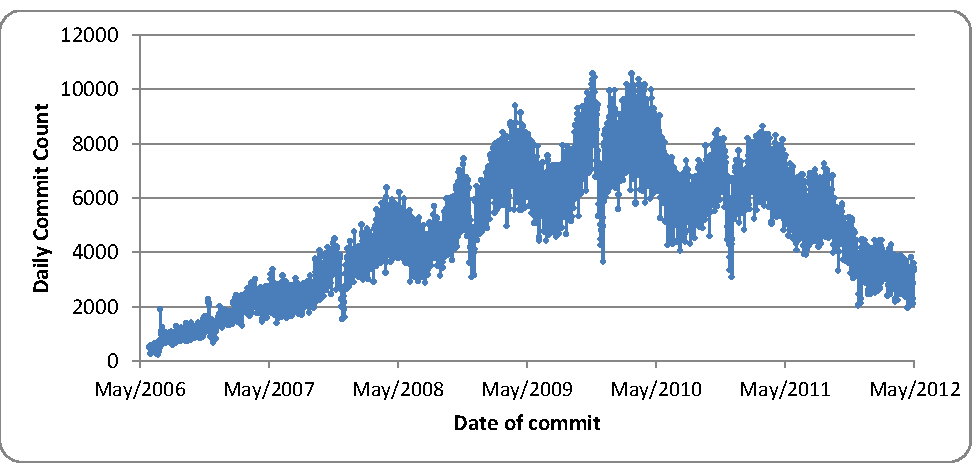
\includegraphics[width=1.0\textwidth]{HistoricGoogleCodeActivityLevels.pdf}
\caption{Commit histogram showing daily activity levels across the entirety GoogleCode.}
\label{fig:HistoricGoogleCodeActivityLevels}
\end{figure}

In the data analysis and visualisations throughout this thesis a fixed upper bound is defined for the time period of study. This was necessary as mining such large volumes of data can take multiple weeks to successfully extract. The majority of this data mining effort took place in the years 2012-2013 and for this reason, it was chosen to only study data up to the end of May 2012. This date was also chosen as it coincides with the availability of then up-to-date FLOSSMole artefacts which, as outlined later in this chapter, facilitates the data mining effort.  

Figure ~\ref{fig:HistoricGoogleCodeActivityLevels} gives an indication of the activity trends but doesn't give an insight into whether this is down to an increase in the number of projects or whether this is attributable to greater activity on existing projects. Figure ~\ref{fig:ProjectCreationHistogram} helps establish that this commit activity is, indeed, visually correlated with an increasing number of projects. Clearly observable is an initial spike of project creation on the go-live date of GoogleCode. In October 2011, a significant drop in project creation is evident, decreasing to an average rate of 3 projects per day. There is no immediately obvious reason in the publicly available records to explain this drop but it is clear that, even prior to this drop, there was a general downwards trend.

\begin{figure}[htbp!] 
\centering    
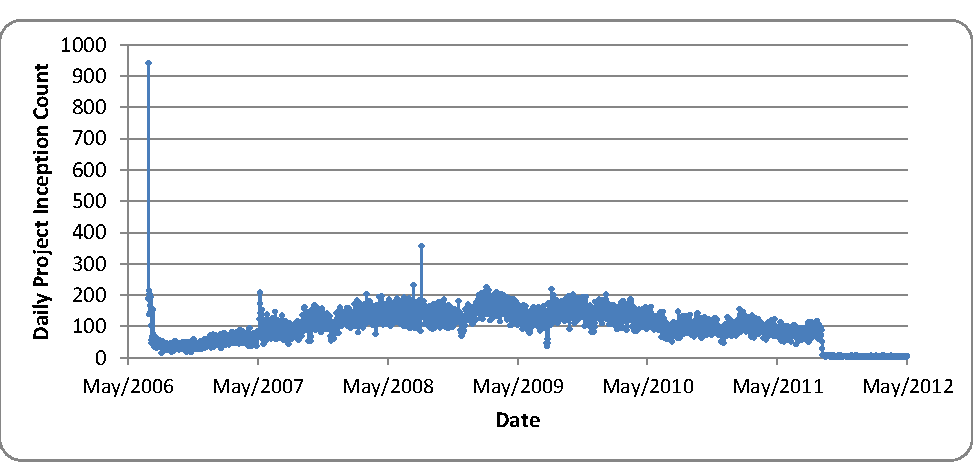
\includegraphics[width=1.0\textwidth]{ProjectCreationHistogram.pdf}
\caption{A histogram depicting the daily rate of new project creation.}
\label{fig:ProjectCreationHistogram}
\end{figure}
	
From a total project count of 236,787 only 95,490 have a single commit (corresponding to the initial project creation). Squire postulates that this is due to 'bots' creating projects although the motive for this activity remains unexplained \citep{squire2017lives}.

\subsection{Toolchain requirements}
This research presented a number of challenges to mine the commit details for all the projects in GoogleCode's repositories and consolidate this information within a single data model and, ultimately, in a relational database for further analysis. 

Given that this research tackles the study of team stability, it is necessary to mine the entirety of the chosen repository in order to derive team stability analytics based on the number of times each committer has worked with every other committer. This research clearly does not stop at an analysis of commit data. Given the focus on the internal attributes of software it is essential to inspect the source files for each project chosen for study, from which structural metrics can be extracted. This data, when juxtaposed with the relevant commit data, allows the trends surrounding structural metrics to manifest as projects evolve and mature. Given the sheer size of GoogleCode this is no small task and it will involve hundreds of gigabytes of data transfer, multiple gigabytes of storage and many days of processing to produce an accurate representation of individual contributor behaviour.

The requirements of the toolchain can be articulated as follows.
\begin{itemize}
\item \textbf{Mine VCS logs and software metrics:} Mine VCS revision history and conduct static source code analysis against each snapshot of source code.
\item \textbf{Breadth and scale:} Capability of mining VCS revision history of thousands of repositories across SVN, Mercurial and GIT.
\item \textbf{Queriable data sets:} Store revision history in normalised queriable form.
\item \textbf{Joinable data sets:} Join VCS revision history data with software metrics mined from snapshots of source code.
\end{itemize}

\subsection{Open-Source Tools}
Table ~\ref{tab:VCSMiningToolSummary} provides an overview of several relevant open-source mining tools - Softchange \citep{german2004mining}, Hipikat \citep{vcubranic2003hipikat}, Dynamine \citep{livshits2005dynamine}, Kenyon \citep{bevan2005facilitating} and CVSAnaly \citep{robles2004remote} - along with a brief summary of their limitations with regards to this research.

\begin{table}
\centering 
\captionof{table}{A comparison of a number of version control mining tools}
\begin{tabular}
 \centering 
 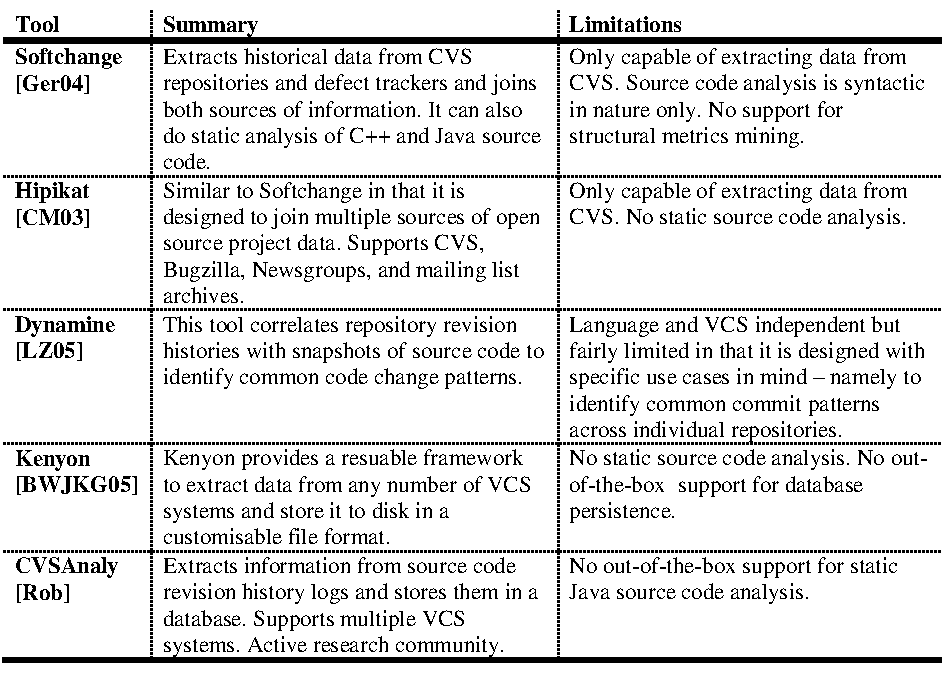
\includegraphics[width=1.0\textwidth]{VCSMiningToolSummary.pdf}
 \label{tab:VCSMiningToolSummary}
\end{tabular}
\end{table}

Of these tools CVSAnaly was considered the more versatile to mine, normalise, and store revision history. The main functional limitations associated with CVSAnaly in the context of this research are as follows.

\begin{itemize}
\item \textbf{Missing support for the Mercurial VCS:} This is one of the GoogleCode supported VCS systems alongside GIT and Subversion - both of which are supported by CVSAnaly.
\item \textbf{Missing support for Static Code Analysis:} Although there was no out-of-the-box support for Java static code analysis, there is support for 'extensions'. For this approach to be successful, such an extension would need to check-out each version of the codebase, execute static code analysis, and commit the results to a version of the CVSAnaly schema.
\item \textbf{Restricted Database Schema:} Integrating static code analysis would necessitate further building out the CVSAnaly schema to store the mined metrics 
\end{itemize}

Consideration was given to committing to enhancing CVSAnaly with the aforementioned functionality - an undertaking that would require that the CVSAnaly codebase be sufficiently understood in order to correctly identify the integration points for various new functionalities. Given the complexity of this task along with the limited existing functional scope, the balance ultimately tipped in favour of creating a bespoke toolchain for data mining. 

\subsection{Toolchain}
This section documents the toolchain developed to mine and analyse the GoogleCode forge. Particular attention is devoted to those components that are common to both team size and team stability analysis: those components that are particular to either type of analysis are discussed in Chapters 4 and 5 respectively.

\begin{figure}[htbp!] 
\centering    
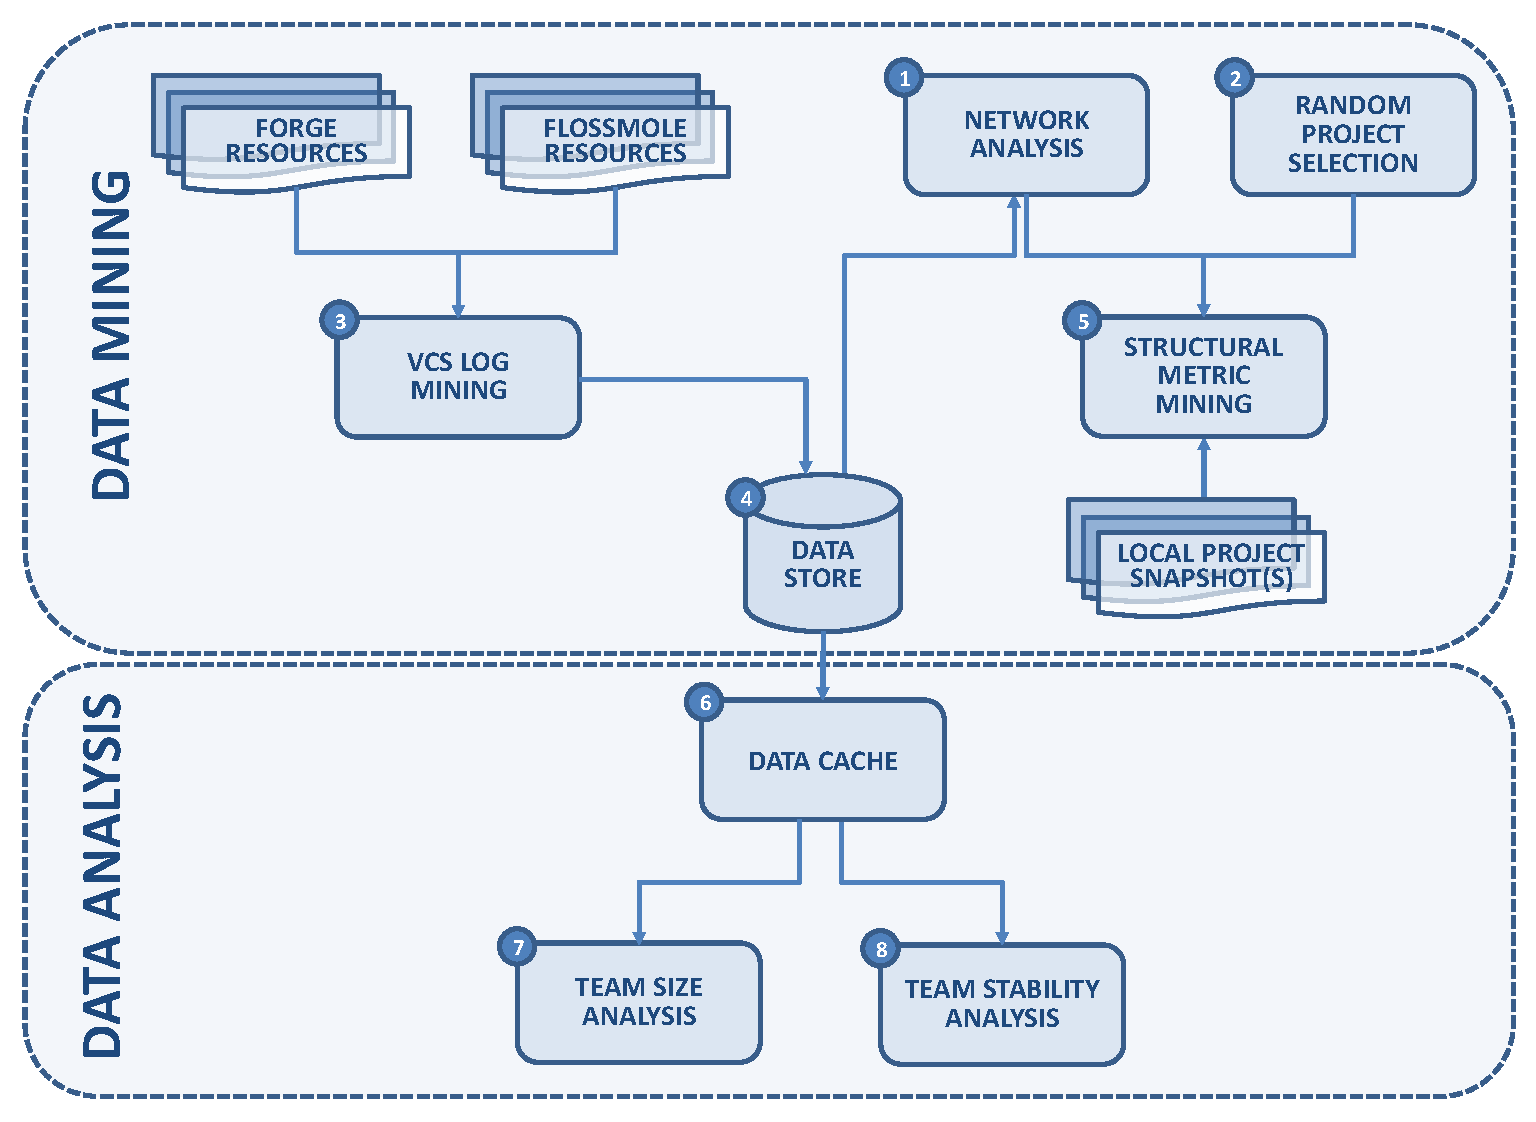
\includegraphics[width=1.0\textwidth]{Toolchain.pdf}
\caption{Toolchain to mine and analyse the GoogleCode forge.}
\label{fig:Toolchain}
\end{figure}

\begin{itemize}
\item \textbf{1. VCS Log Mining:} The FLOSSmole project makes available the raw data describing, at a project level, details of all projects hosted in GoogleCode. This, along with the GoogleCode project webpages and the associated repositories formed the input into the bespoke toolchain illustrated in Figure ~\ref{fig:Toolchain}. At its essence, the VCS mining component is a collection of shell scripts, run on a UNIX platform and driven by the FLOSSMole flat files and the GoogleCode project webpages, designed to retrieve, parse and persist the full revision history of all the projects in the forge. To mine this data, these scripts access all project repositories in the forge to retrieve the full revision history, parsing it accordingly and storing it in the database to then drive subsequent analysis. To achieve this, the scripts make use of command line tools made available by the VCS to retrieve meta-data about each project revision. Spinellis and Gousios adopt a similar approach to mining VCS meta-data, discussing its necessity in detail \citep{spinellis2018analyze}.

These scripts support three version control systems: Subversion, GIT, and Mercurial. In the case of Subversion and GIT, the revision history can be directly queried through the appropriate binaries (albeit through different syntax and requiring individual log parsers) while in the case of Mercurial it is necessary to clone the repository before retrieving the history. The revision history extraction scripts use the repository URI to determine the type of version control system and extract the data appropriately.

\item \textbf{2. Network Analysis:} The network analysis conducted in this research is focused on accurately mapping committer activity and project engagement in the context of the activity of the broader development team. This is used to calculate the stability of a team through the evolution of the project as well as understanding the change in team composition from one project to the next. This analysis also enables the mining of the full data set for projects that fulfil the criteria necessary for team stability analysis; for instance, pairs of projects where the development team remained stable. This will be discussed further in Chapter 5 as the team stability analysis is detailed.

\item \textbf{3. Project Sampling:} This is a Java component designed to extract, in a reproducible fashion, a representative sample of projects from the full data set of 236,787 projects in the GoogleCode forge. There is functionality to identify and select projects programmed in a particular programming language (Java) to simplify structural metrics mining. This component is covered in detailed in Section 4.2 of the next chapter.

\item \textbf{4. Structural Metric Mining:} This component comprises of, again, UNIX shell scripts responsible for checking out each version of the project, handing over the heavy lifting of metrics generation to an out-of-the-box metrics generation tool. Using an existing tool for structural metrics mining was favoured over writing a bespoke tool given that, unlike VCS mining, metrics calculation is complex and potentially error prone. This meant that creating a bespoke tool would require significant build and validation effort. Fortunately the landscape of available tools was sufficiently rich such that a suitable tool could be identified with ease and without the need for extensions or enhancements. Table ~\ref{tab:MetricMiningToolSummary} shows a comparison of the available metric generation tools categorised by the distribution license (commercial or open-source) and deployment (standalone or integrated into an IDE) \citep{spinellis2005tool, scitools, powersoftware, metricssourceforge, ndepend}. 'Understand' by Scientific Toolworks Inc. was chosen as it is amongst the most reputable and widely adopted, was available on academic license, and offers a command line tool that generates metric reports in an easily parsable format. The report created by Understand is then passed through a Java Parser which extracts the information that is pertinent to this research and stores it in a format appropriate for use by the metrics analysis component. The calculations used by Understand to generate metric values are documented in Table ~\ref{tab:Understand}.

\begin{table}
\centering 
\captionof{table}{A comparison of a number of structural metrics mining tools}
\begin{tabular}
 \centering 
 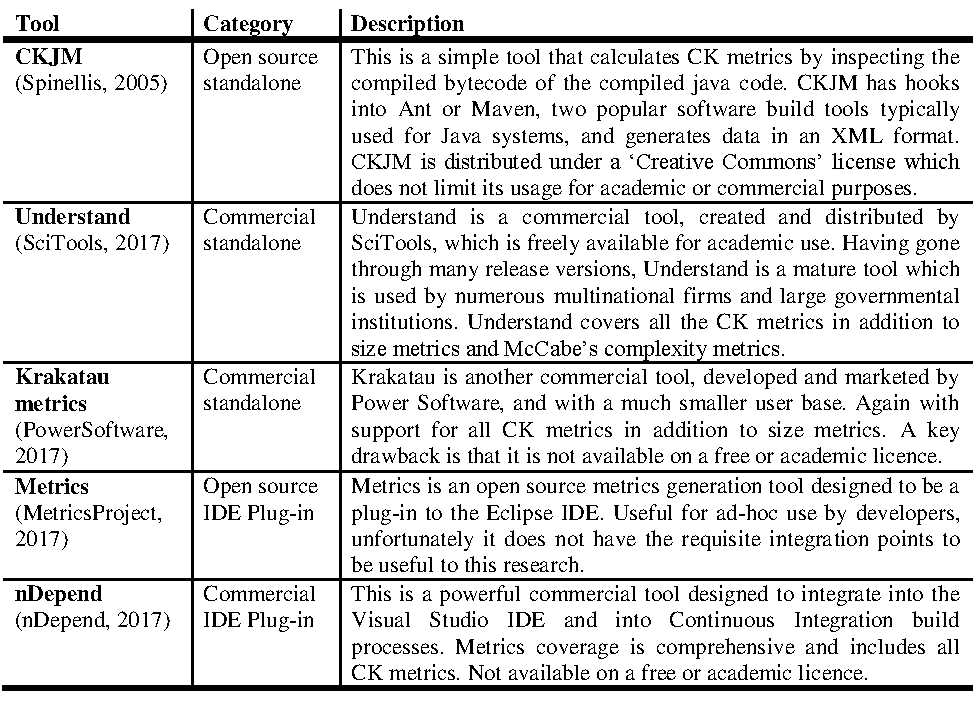
\includegraphics[width=1.0\textwidth]{MetricMiningToolSummary.pdf}
 \label{tab:MetricMiningToolSummary}
\end{tabular}
\end{table}

\begin{table}
\centering 
\captionof{table}{A description of how CK Metric values are calculated for Java classes by Understand.}
\begin{tabular}
 \centering 
 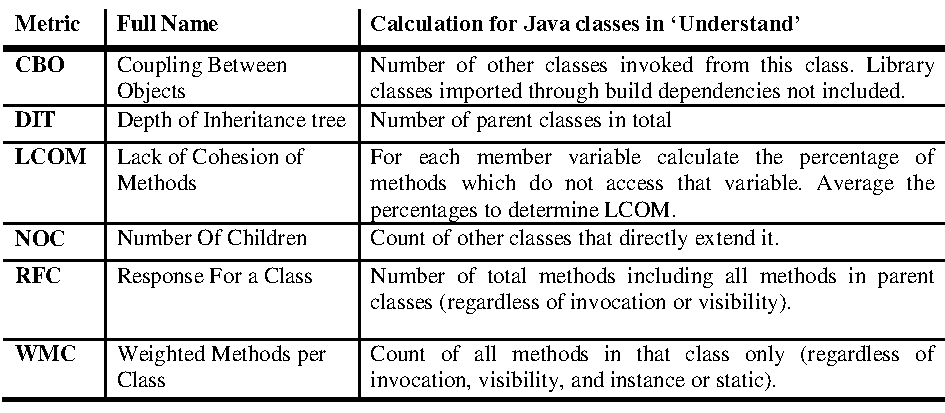
\includegraphics[width=1.0\textwidth]{Understand.pdf}
 \label{tab:Understand}
\end{tabular}
\end{table}

\item \textbf{5. Data Store:} Raw metrics and analysis should be stored in a queriable format to facilitate further data analysis - particularly statistical analysis - to identify trends and correlations. A MySQL database was created with a schema reflecting the data model outlined in Figure ~\ref{fig:Schema} to store the results of the VCS log mining and the structural metric mining. 
 
 \begin{figure}[htbp!] 
 \centering    
 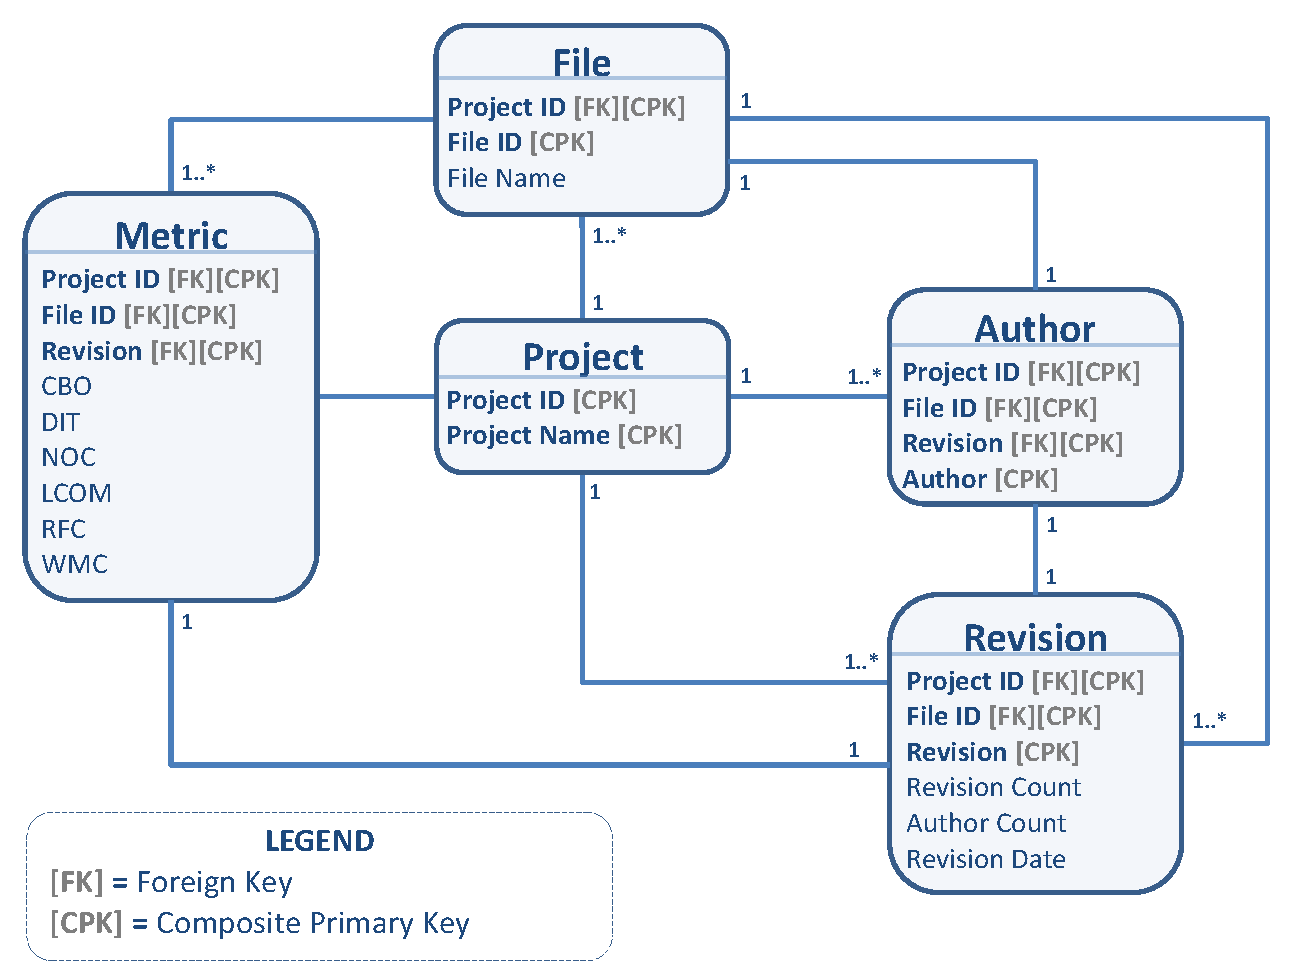
\includegraphics[width=1.0\textwidth]{Schema.pdf}
 \caption[A simplified ER diagram depicting the logical data model used by the data store.]{A simplified ER diagram depicting the data model used by the data store. This is closely reflected by the object model underpinning the analysis components.}
 \label{fig:Schema}
 \end{figure}

\item \textbf{6. Data Cache:}
When conducting analysis - and in particular network analysis - it is necessary to traverse a large data set multiple times in order to make meaningful observations on the data.

For example, to establish which committers have common project engagements, it is necessary to traverse the data set and categorise project engagements by committer. To calculate the stability of a team within a project, a traversal of the data for that project is required to determine the overlapping committer engagement periods. For this reason, it is efficient to load entire commit data into an in-memory data structure within the Java Virtual Machine running the team size and stability analysis to facilitate rapid access and flexible indexing. In practice this is implemented using hash maps keyed by author and project as appropriate for the requisite type of analysis. 

\item \textbf{7. Team Size Analysis:} This is the subject of Chapter 4 so will not be discussed at length here. However, as a brief overview it is worth mentioning that a Java component queries the database and joins structural metrics with commit-level information in order to produce an aggregated result set. This result set is then analysed using the Anaconda Data Science workbench \citep{anaconda} running Python 'notebooks', the source code for which is available on GitHub in the location previously specified in the chapter titled 'Publications'. Figure ~\ref{fig:Analysis} illustrates the approach to data analysis across both team size and stability.

\item \textbf{8. Team Stability Analysis:} Similarly, this analysis is the subject of Chapter 5 but suffice to say that the design is similar to the previous component with a focus on reading commit data and its associated meta-data to calculate team stability measures. This then drives the categorisation and statistical comparison of structural metrics in order to ascertain the impact of stability on metric values.
\end{itemize}

 \begin{figure}[htbp!] 
 \centering    
 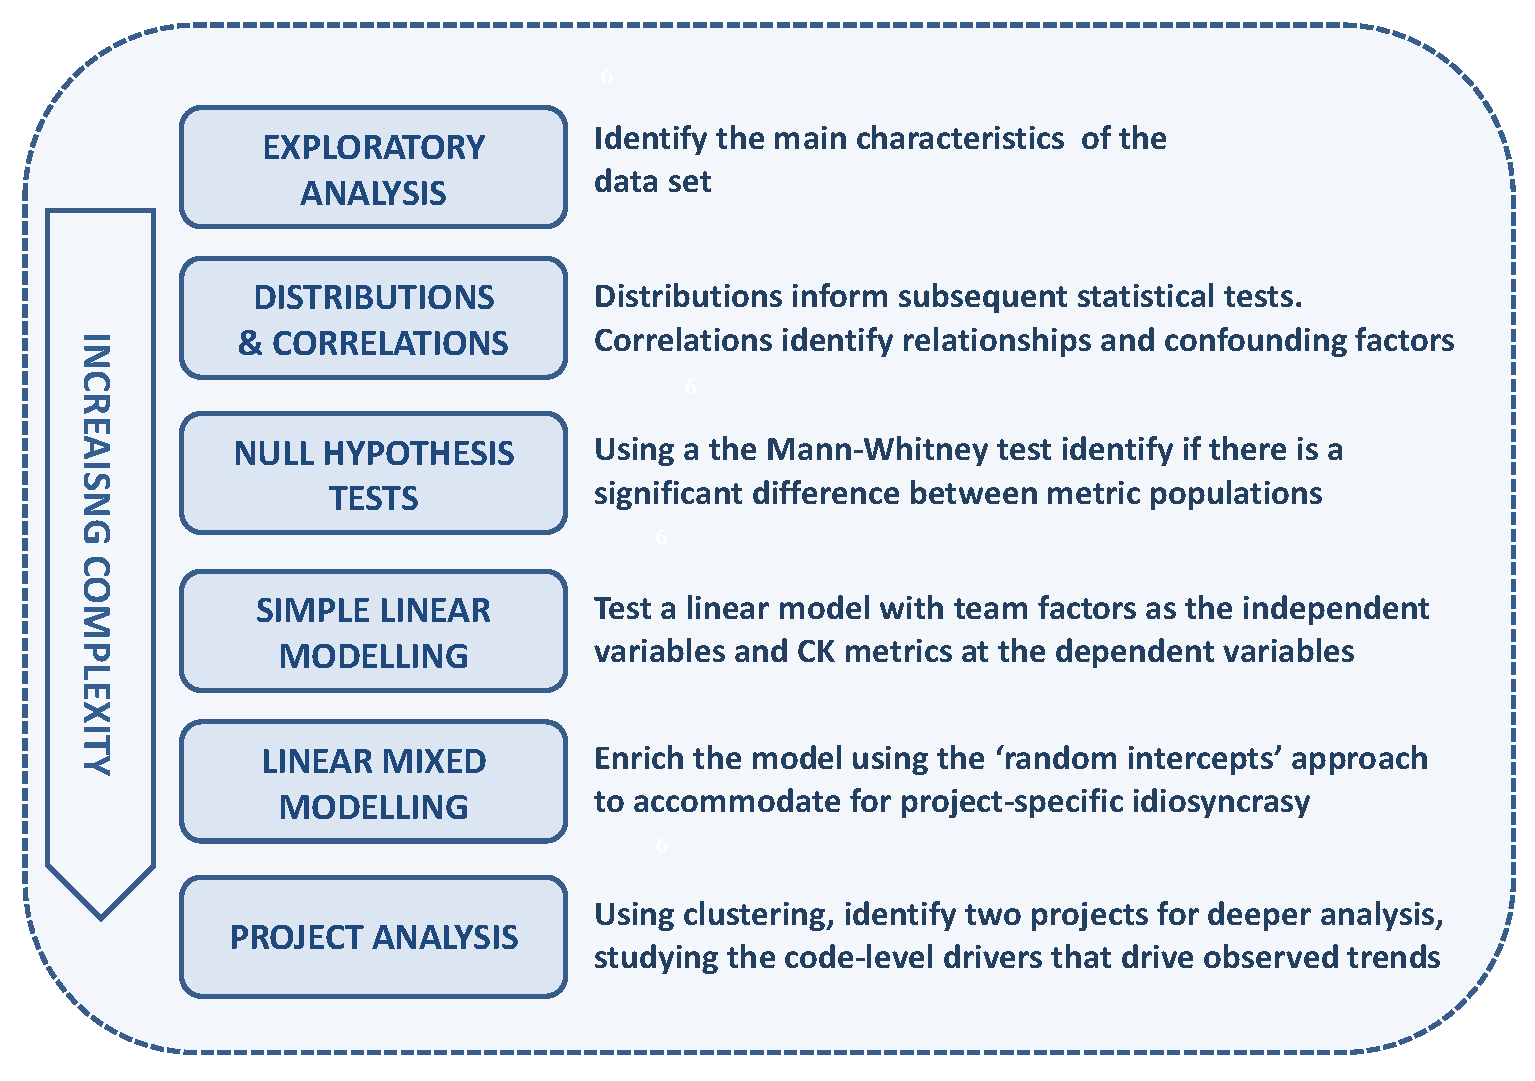
\includegraphics[width=1.0\textwidth]{Analysis.pdf}
 \caption[A summary of the data analysis approach.]{A summary of the common approach to data analysis across both team size and stability.}
 \label{fig:Analysis}
 \end{figure}

\subsection{Validating the Toolchain}
The toolchain described bears a basic high-level similarity to one independently developed by Ludwig et al. to extract metrics of maintainability from GitHub repositories \citep{ludwig2017compiling}. One challenge involved in developing a bespoke toolchain was the requisite effort to ensure its validity. Whenever writing code, typically good engineering practices such as ensuring adequate unit test coverage should be a given \citep{tosun2018effectiveness}. The approach taken to development of components for this research was no different. This gives some level of confidence that individual elements in the toolchain have been correctly implemented. 

However, to get adequate confidence that the complete toolchain is functionally sound from an end-to-end perspective, it was necessary to manually validate the toolchain results against a small project. To ensure that the validation process was not overly taxing yet suitably thorough, the project to validate was chosen to have a limited number of project revisions yet have multiple authors including multiple revisions and authors on the same source file. The project selected for this purpose was zsea-planetwars as it has 8 revisions and 3 authors. The project was downloaded in each of its 8 snapshot states and imported within the Eclipse IDE. For each file within each snapshot, the metrics were derived by hand and validated successfully.

\subsection{Toolchain Performance}
The toolchain uses standard programming languages and does not require any specialised hardware or operating systems. However, as mining processes are network bandwidth intensive, the software was deployed to a commercially hosted Virtual Private Server (VPS) as this guaranteed faster internet connectivity than could be achieved with a typical domestic connection. The VPS account was an entry-level single core deployment with 512MB RAM, 25GB of data storage. The Linux distribution was CentOS 6.8.

The time taken to download VCS logs is dependent on the volume of revision history for a given project but is generally in the single digit seconds. Mining structural metrics is a more time-consuming process and can take around several minutes for a single 'snapshot' of the source code. This is a roughly equal distribution between the time taken to download the source code and the time taken to run static code analysis. Medium sized projects can have hundreds of revisions which leads to a total analysis time in the hours. As a rough guide, mining structural metrics for a 1000 project sample takes about 300 hours. Even with the limitation of a single core, this process can be made much faster by running parallel processes (multi-threading). 25 threads was found to be optimal and resulted in a sample processing time of approximately 24 hours.

Once stored in the MySQL relational database the data associated with all revisions of a single project within the sample takes up approximately 4-5MB of disk space. While this may present a technical challenge when mining the entirety of the forge for structural metrics, this was not a concern when limiting the static analysis to a representative sample of projects.

\section{Metrics} %Section - 3.4
\subsection{Overview}
While ISO/IEC 25010 recognises that internal quality drives external quality, it does not offer any specific direct measures for internal quality but instead offers a framework to define metrics that are influenced by internal quality. For example, maintainability is measured by the resources expended to modify software. These measures are neither direct nor predictive. Fortunately, there has been significant research in formulating such direct measures. 

Coleman et al., in the early 90s, developed a maintainability model that used static measures of source code to produce a percentage figure on how easy  a system is to support and change derived from a blend of measures including complexity metrics \citep{coleman1994using}. This metric is still used today within Visual Studio which classifies ranges which correspond to High, Moderate and Low maintainability \citep{msdn2015code}. Heitlager et al. from the Software Improvement Group (SIG) critiqued this model as presenting difficulties in re-constructing the root causes that drive a particular measure and suggested an alternative maintainability model which blends structural metrics including complexity, volume, and unit size to drive its metrics \citep{heitlager2007practical}. The strength in the SIG maintainability model is the simplicity with which a calculated index would be mapped to its constituent structural attributes.

In a similar vein, the approach of this research to observing indicators of internal quality is to directly measure the internal structural attributes of a codebase and draw upon established models to ascertain if the trends observed indicate enhanced or degraded internal software quality.

There are two primary categories of internal attributes of software - size and structure. Software size is a broad term and measurements can vary from basic line of code counts through to function-point analysis. It is tempting to assume that size is directly correlated to external attributes of fault-proneness and development effort while negatively correlated to maintainability \citep{akiyama1971example}. However, as Fenton and Bieman state, experience shows that this is not a valid assumption and that the structural attributes of software play a vital part in driving these external attributes \citep{fenton2014software}.
 
This section first discusses the metrics which can be used to capture structural attributes followed by a brief historical context. The metric suite chosen for the purposes of this research is then discussed and detail is given to how previous research has linked these metrics to external quality attributes.

\subsection{What Are Structural Metrics?}
Software metrics embody an empirical approach to software engineering and are primarily designed to assist in making assessments of software artefacts and development processes, in the process guiding engineers and project managers in their decision-making. A software metric is the quantitative measure of the degree to which a component, system, or process possesses a given characteristic or attribute \citep{ordonez2008state}. If used appropriately, software metrics can lead to a significant reduction in costs of the overall implementation and maintenance of the final software product. 

Structural metrics are a specific category of software metrics that allow us to measure and express the adherence of a codebase's structural attributes to sound engineering design principles. The key attributes in Object Oriented Programming are the interlinked concepts of coupling, cohesion, complexity, and modularity. These are explained as follows.

\begin{itemize}
\item \textbf{Coupling:} This is the degree to which components within software systems are interdependent. A high degree of coupling in a set of components implies that changes in one component may impact the other components in that set \citep{parnas1972criteria}. At a relatively low level, modern object-oriented languages provide paradigms (such as interfaces) to facilitate lower coupling between classes. Interfaces allow a developer to separate the method of interaction into a component from the implementation of functionality. At a higher level, enterprise design patterns such as the Service-Oriented Architecture facilitates lower levels of coupling between applications \citep{jamshidi2018microservices}. Lower levels of coupling are desirable at each level of an enterprise software system \citep{chidamber1998managerial, pressman2005software}.

\item \textbf{Cohesion:} Cohesion is a measure of the extent to which functionality within a single component belongs together. A component that exhibits a high degree of cohesiveness typically encapsulates a single set of highly related functionalities. In object-oriented languages, a high degree of cohesiveness is a desirable trait and is consistent with the 'single responsibility principle' which states that a class should have a single purpose and its functionality should be encapsulated within the class - i.e. not exposing its inner workings to other components \citep{fenton2014software}. A high degree of cohesiveness and encapsulation is associated with a low level of coupling \citep{chidamber1998managerial}.

\item \textbf{Complexity:} In the context of structural metrics, complexity refers to the structural complexity of software rather than the functional complexity. This is a contrast that will be discussed in the coming chapter in Section 4.4.3.2. Structural complexity is a measure of the degree of interactions between components in a software system \citep{fenton2014software}. A highly complex system would contain a large number of components and a large number of interactions between the components. Although the number of interactions between components is a driver of structural complexity, the nature of the interaction between two components can introduce further structural complexity if there is a dependency on the inner workings of the components (i.e. poor encapsulation and high coupling). Although functional complexity can often introduce structural complexity, all things being equal, lower measures of structural complexity are desirable.

\item \textbf{Modularity:} This refers to the extent to which a system's functionality is logically partitioned into independent components \citep{parnas1972criteria}. A high degree of modularity is desirable as it encourages low coupling and high cohesion which, in turn, reduces structural complexity \citep{parnas1972criteria, sullivan2001structure}.
\end{itemize}

\subsection{Survey of Metrics Suites}
There are a number of structural metric suites that commonly appear in both academic literature and practitioner tools. In this section a comparative survey is provided for the most popular metric suites and justification is given to the choices in this research. The discussion is limited to object-oriented structural metrics given that, as mentioned earlier in this chapter, this research studies Java software only. This is to the exclusion of suites such as the Halstead metrics. Furthermore, consideration is only given to those metric suites that comprehensively cover the key internal structural attributes - coupling, cohesion, complexity and modularity - to the exclusion of, for example, the McCabe metrics with their almost exclusive focus on structural complexity \citep{mccabe1976complexity, mccabe1989design}. For a fuller survey of the available object-oriented structural metric suites, the reader is encouraged to review the work of Gomathi and Linda Edith \citep{gomathi2013an} and Xenos et al. \citep{xenos2000object}. The comparison is therefore limited to the Chidamber and Kemerer suite, the MOOD metric suite and the Lorenz and Kidd metric suite.

\begin{itemize}
\item \textbf{Chidamber and Kemerer metric suite} The Chidamber and Kemerer (CK) metric suite is one of the most cited of all structural metric suites within the academic community \citep{pressman2005software} with a great deal of research spanning the two decades since its creation. 

The CK metric suite is designed to operate on the most fundamental unit in object-oriented systems - the class. The CK metric suite contains measures that capture complexity, coupling and cohesion. The values of the measures are fairly arbitrary and there has been research into defining the thresholds that could indicate classes which would be more likely to require remedial action \citep{rosenberg1998applying}. While there has been some doubt cast on the theoretical and empirical validity of one of the measures in the suite \citep{fenton2014software}, nonetheless, this remains the most validated OO metric suite available \citep{kitchenham2010s} with a great deal of research successfully correlating the metrics to external quality attributes \citep{rosenberg1998applying, el2001prediction, basili1984software, subramanyam2003empirical}. This suite is covered in more detail later in this chapter.

\item \textbf{MOOD metric suite} The MOOD metric suite was developed by Abreu and Carapu\c{c}a in 1994 to provide system-level measures (as opposed to class-level measures) for object-oriented systems in order to guide and assess OO design quality \citep{abreu1994object}. The measures capture a broad range of structural attributes including encapsulation and polymorphism factors - factors absent from the CK metrics suite. In contrast to CK metrics where the values of the measures are arbitrary, the MOOD metric values are probabilities with values from 0 to 1 representing the likelihood of the existence of a particular attribute. Harrison et al. conducted research detailing the utility of MOOD metrics to practitioners finding that they present information that would be of general use to software managers to understand the overall attributes of a system \citep{harrison1998investigation}. MOOD metrics are not widely adopted in academic research nor industry and this is reflected in the very scarce availability of tools that generate these metrics with Project Anaylzer \citep{abounader1997data} being the only distributed tool that the author could find. This tool only had support for the Visual Basic programming language. In its favour there has been significant research analysis which largely validated the MOOD metric suite \citep{abounader1997data, harrison1998evaluation}.

\item \textbf{Lorenz and Kidd metric suite} In their book 'Object-Oriented Software Metrics' Lorenz and Kidd proposed a metric suite consisting of eleven metrics that, in a similar fashion to the CK metric suite, measured attributes at a class level \citep{lorenz1994object}. Metrics are broadly in four categories - size, inheritance, class internals (attributes that can be measured on a class in isolation such as cohesion) and class externals (attributes that capture how a class interacts with other classes such as coupling and reuse). Lorenz and Kidd also propose threshold values to help interpret metric observations. The Lorenz and Kidd suite did experience a degree of recognition in academic circles with a large number of citations \citep{nesi1998effort} but, with few validation studies \citep{sharma2012metrics} and no available tools to measure these metrics, it is fair to say that this metric suite has not experienced significant academic or practitioner adoption. This may be due to the fact that the metric suite is fairly basic and constitutes directly measurable attributes such as Number of Methods, Number of Public Variables and Number of Variables which has caused some doubt to be cast on its usefulness \citep{harrison1998investigation}.
\end{itemize}

\subsection{Choosing a Metrics Suite} The research questions in this thesis mandate a number of key criteria of the metric suite chosen for this work. The first main requirement is that the suite is comprehensive in capturing the key attributes in Object Oriented Programming, described earlier in this chapter, of coupling, cohesion, complexity, and modularity. The second key criterion, necessary for the validity of this research, is that the metric suite be credible and empirically validated in an existing body of research. This means that the metrics must be proven reliable indicators of external quality attributes.

For this work to maintain relevance to its intended audience, which encompasses both researchers and practitioners, it is helpful to employ a metrics suite that can be well understood by practitioners, with individual metrics directly mapping onto the internal attributes. Furthermore, the chosen metric suite is that it should have good tool support as eases the development of a toolchain, enhances the repeatability of this work, and also serves as a gauge of its popularity amongst researchers and practitioners alike. 

The matrix in Table ~\ref{tab:MetricSuites} below details how each of the three metric suites considered match up to this criteria. The CK metrics suite is the only suite that is an adequate match - particularly with respect to empirical validation, relevance to practitioners and tool availability. For these reasons the CK metrics suite forms the basis for the empirical approach to this research. 

\begin{table}
\centering 
\captionof{table}{A comparison of the three metric suites considered for this research against the stated criteria.}
\begin{tabular}
 \centering 
 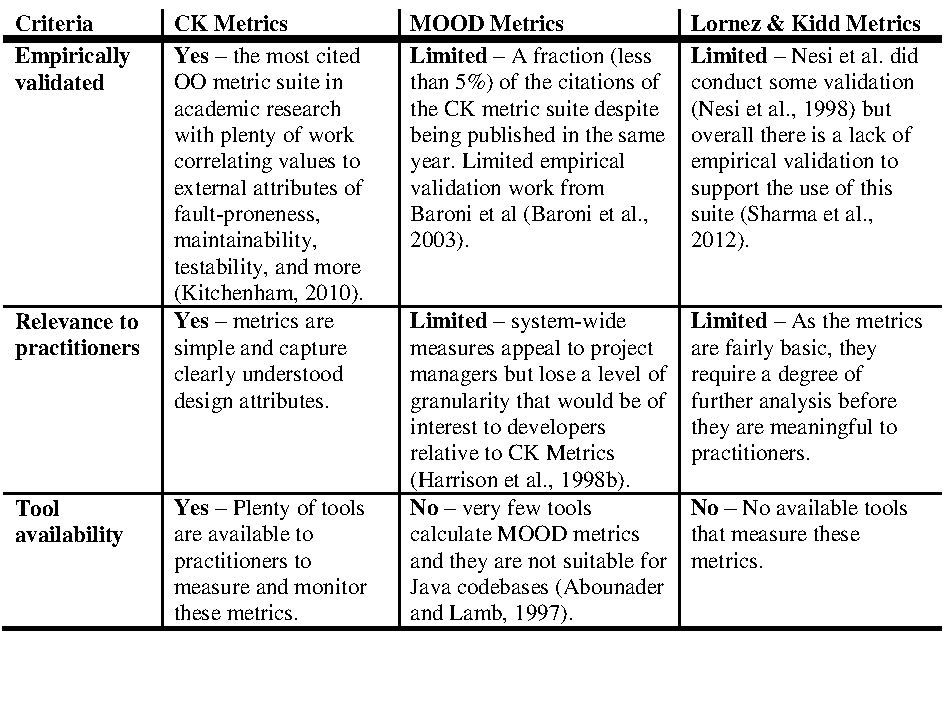
\includegraphics[width=1.0\textwidth]{MetricSuites.pdf}
 \label{tab:MetricSuites}
\end{tabular}
\end{table}

\section{Chapter Review} %Section - 3.5
This chapter covered three fundamental aspects to the methodological approach of this research. First, measurable definitions of team size and stability were established, laying the groundwork to the empirical work in this thesis. The FLOSS mining toolchain was then detailed, covering aspects of performance and validation. Figure ~\ref{fig:Analysis} illustrated the general approach to data analysis across the team size and stability analysis that will follow in the coming chapters. Finally, structural metrics are covered in detail and the process leading to the selection of the CK metrics for this research is covered.

The next chapter uses the methodology described in this chapter, along with a number of linear models, to establish a relationship between team size and the structural attributes of software. 
%!TEX root = ../thesis.tex

\graphicspath{{Chapter4/Figures/}{Chapter4/Tables/}{Chapter4/Charts/}}

\chapter{The Impact of Team Size on Structural Metrics}
\section{Introduction} %Section - 4.1 

The first research question (RQ1) seeks to establish '\textit{the impact of development team size on the internal structural attributes of software projects and the implications on its maintainability}'. In practice this means first establishing if populations of structural metrics of software, when grouped by team size, exhibit statistically significant differences. Where such a difference is observed, the nature of that difference should be ascertained.

This chapter follows a methodical approach of initially conducting foundational work to facilitate that statistical analysis. The subsequent sub-sections articulating the analyses are of incrementally increasing complexity as outlined in Figure ~\ref{fig:ChapterOverview}. Section 4.2 is titled 'Data Mining' which details efforts to extract a data sample from the broader forge and to mine the sample for structural metrics. Section 4.3 covers an initial 'Exploratory Data Analysis': efforts to understand the underlying trends in the mined data from a one-dimensional perspective in addition to the distribution and correlations within. Section 4.4 documents an initial, 'Univariate Analysis' to establish a relationship between team size and structural metrics - simplistic as the confounding impact of revisions (potentially a proxy to functional complexity) means that this analysis will not yield clear or reliable results but will serve to establish the foundation on which the further analysis will take place. These confounding factors will be the subject of Section 4.5 which factors in the impact of revisions to observe the impact of the development team size, alone, on structural metrics. In Section 4.6 the results are presented in the context of two individual projects and qualitative code-level observations are made to highlight the reasons that drive the quantitative forge-level observations. Finally Section 4.7 provides a summary of the results and relates the observed relationship between team factors and CK metrics to the likely impact on maintainability. Figure ~\ref{fig:MiningToolchain} highlights the aspects of the toolchain that will be subject to further discussion in this chapter.

\begin{landscape}
\begin{figure}[htbp!] 
\centering    
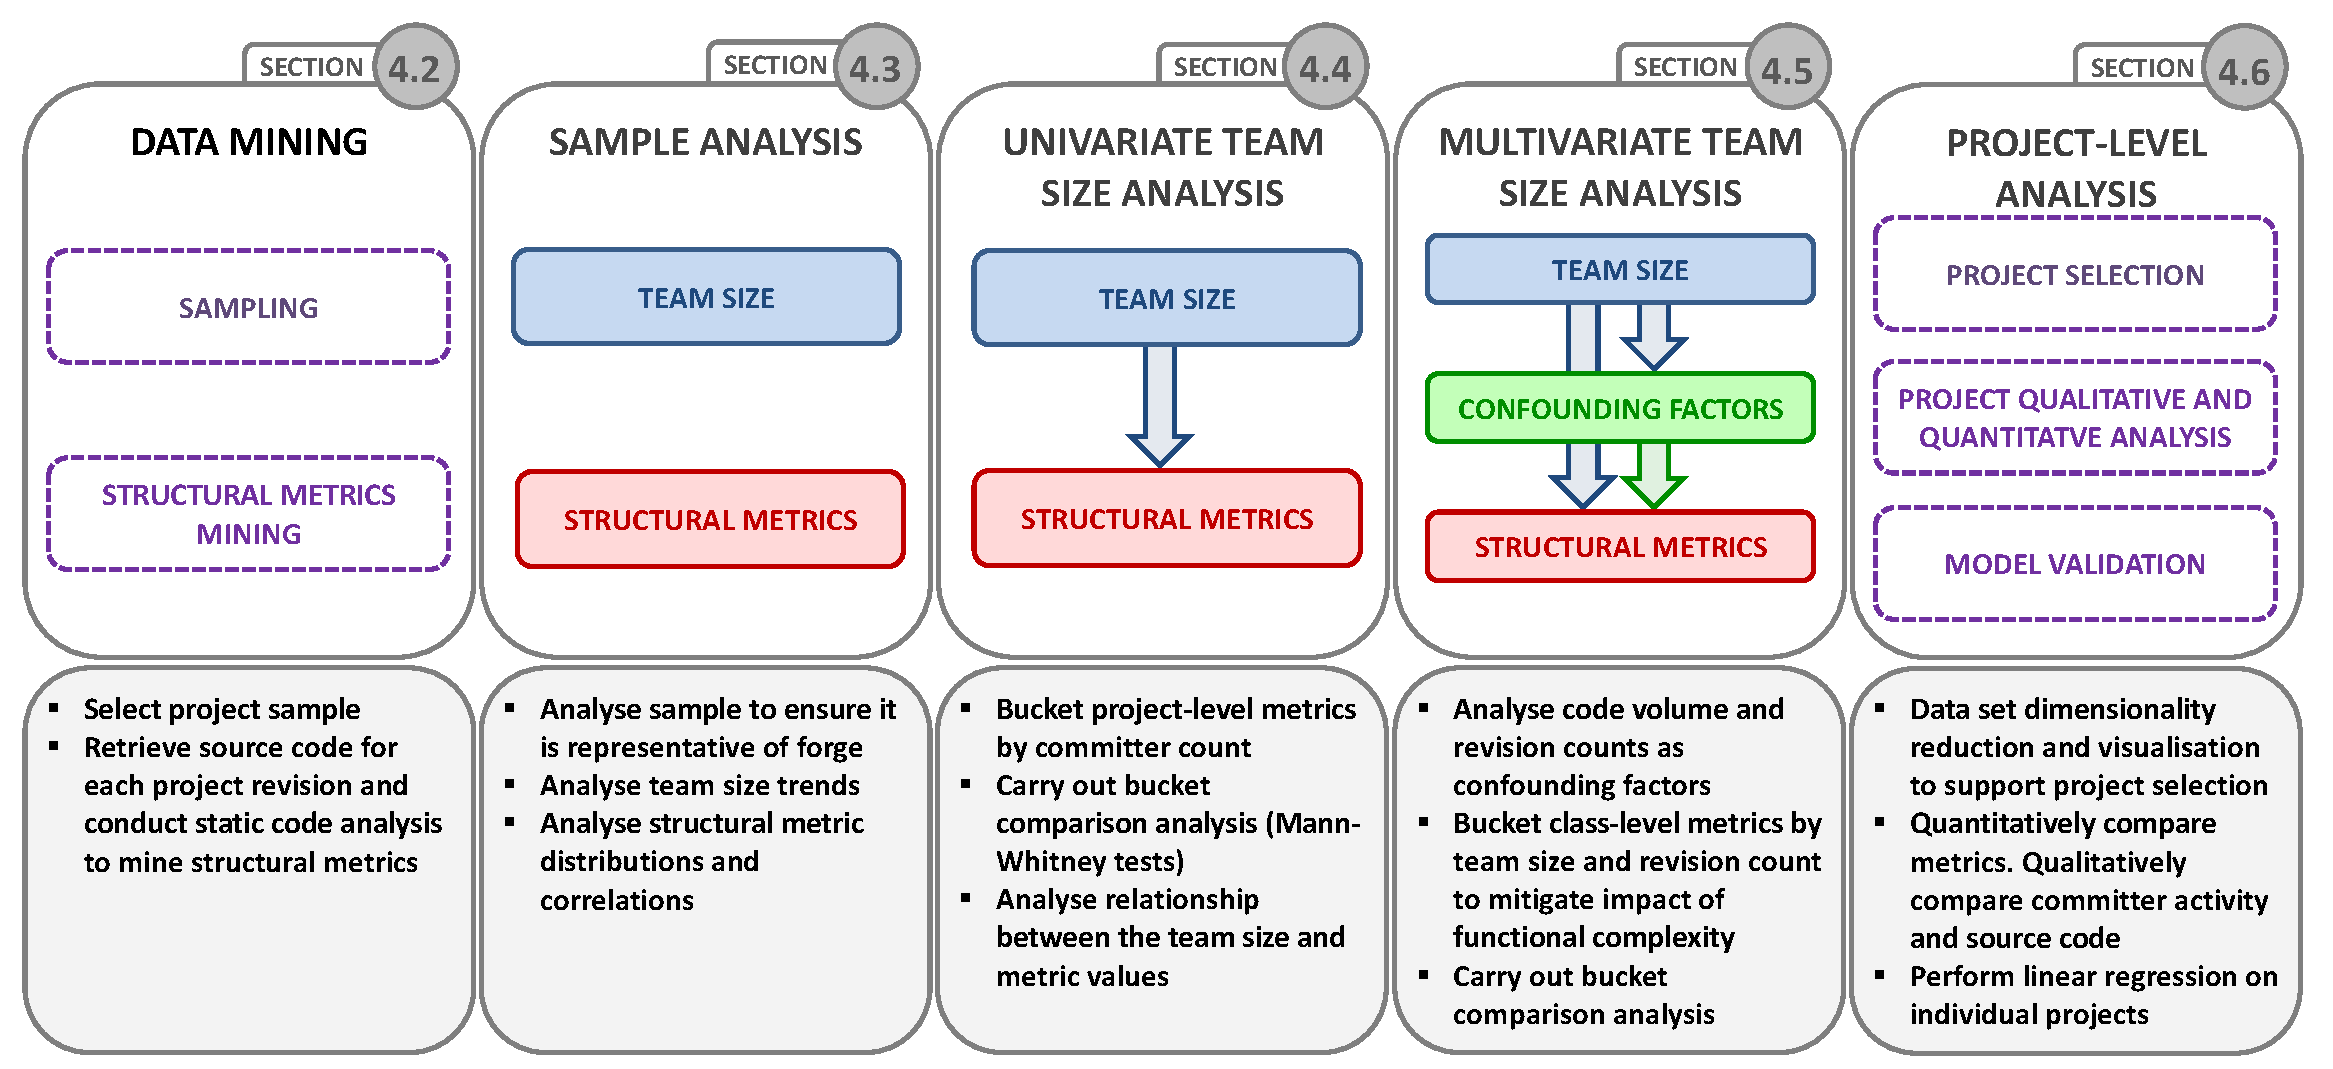
\includegraphics[width=1.4\textwidth]{ChapterOverview.pdf}
\caption{Chapter 4 outline providing an overview of the contents of each section.}
\label{fig:ChapterOverview}
\end{figure}
\end{landscape}

\begin{figure}[htbp!] 
\centering    
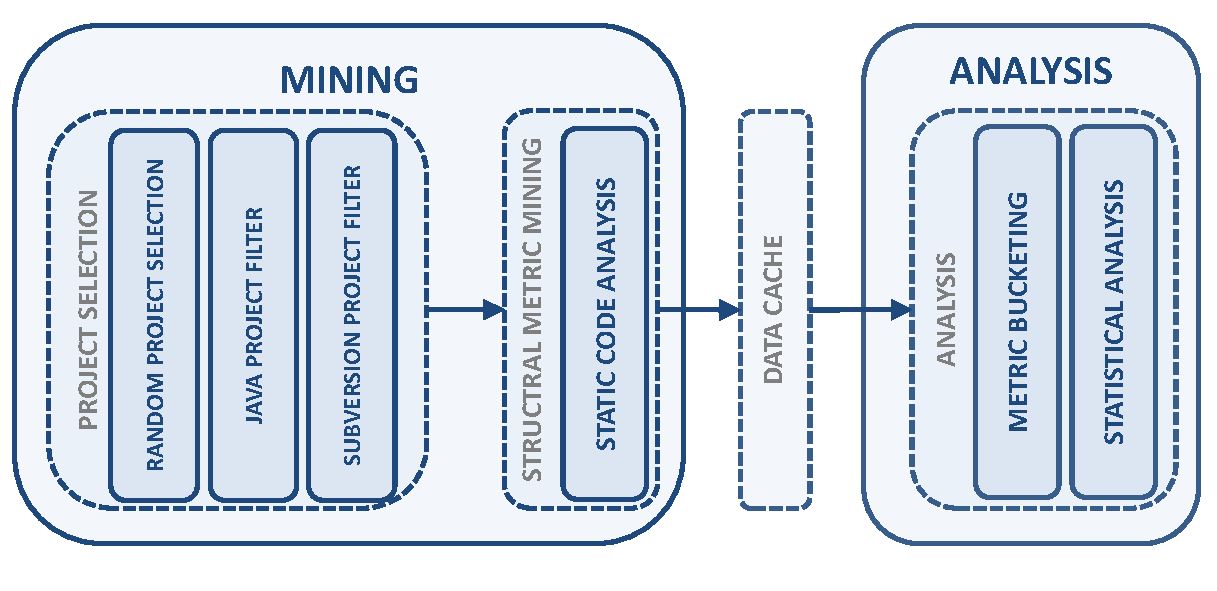
\includegraphics[width=1.0\textwidth]{MiningToolchain.pdf}
\caption[Some aspects of the toolchain pertinent to team size analysis.]{Some aspects of the toolchain pertinent to team size analysis. Project Selection and Structural Metric Mining are both the subject of discussion in section 4.2. Analysis is the subject of the remainder of the chapter.}
\label{fig:MiningToolchain}
\end{figure}
 

\section{Data Mining} %Section - 4.2
When analysing basic committer activity within a forge it is possible to learn a substantial amount through mining the revision logs across all the repositories within the forge. Although requiring significant processing, given modest resources it is computationally feasible to mine the revision history of all projects in a forge made of up several hundred thousand repositories. It is necessary to mine the entire forge when conducting network analysis (as discussed in detail in the next chapter). This, however, is not the case when conducting the detailed structural metric based analysis contained within this chapter. To mine structural metrics necessitates network, processor and storage intensive processes to execute the retrieval and static analysis of the source code at each revision for each project studied. As described in section 3.3.8 in the previous chapter this is still a very resource intensive task and it is not practical or necessary to run this type of analysis across the entirety of the forge. For the purposes of this research it is most appropriate to restrict this type of in-depth analysis to random sample of projects. 

With this context in mind, this section covers two key aspects of the data mining approach that are foundational to the team size analysis: Project Selection and Structural Metric Mining. 

\subsection{Sampling}
The project selection component was outlined in section 3.3.6 of the previous chapter and is a Java component taking, as its input, flat files made available by FLOSSmole providing a full listing of all projects hosted by GoogleCode. Its first responsibility is to identify, within this population, a sample of projects programmed in Java. As discussed earlier, Java was chosen as it increases relevance to the academic and practitioner community and restricting to projects of a single language greatly simplifies the data mining by not requiring support for static code analysis across multiple languages. While restricting the analysis to a single language aids practicality, it also presents a threat to validity when generalising the applicability of any results to projects in any other language, as was highlighted in early research \citep{basili1996validation}. While some similarities carry across object-oriented languages, earlier work has highlighted some of the structural differences between Java and C++ projects \citep{subramanyam2003empirical, english2009exploring} finding that Java lends itself to greater maintainability. These threats to validity are the subject of further discussion in Chapter 6.

While creating projects in GoogleCode the project administrator can associate 'tags' with the project. This is essentially meta-data enabling the categorisation of projects for the purposes of searching or browsing projects. FlossMole provides this meta-data in flat file format. Analysis of this meta-data shows that 204,918 projects (87\%) have at least one tag and on average each project has 4 tags defined. Given that tags are free text, there are a large number of unique tags (145,600). The top 250 most frequent tags were extracted and manually categorised accordingly. The relative occurrences of each category was then calculated on the basis of the 250 most frequent tags and depicted in Figure ~\ref{fig:ProjectCategorisation}. 

The results in Figure ~\ref{fig:ProjectCategorisation} demonstrate that tagging projects by programming language is fairly common. It follows that identifying a substantial set of Java projects is achievable through tag analysis alone. Table ~\ref{tab:GoogleCodeLanguage} shows Java as the most popular language tag associated with 22,594 projects (making it also the most popular tag in any category). This set of projects is considered the \textit{population}.

GoogleCode allowed project administrators to choose from among three available version control systems - Subversion, GIT, and Mercurial - on which to host their source code. Each of these necessitate a different mechanism to mining data. In the case of Subversion and GIT, the revision history can be directly queried (albeit through different syntax and requiring individual log parsers) while in the case of Mercurial it is necessary to clone the repository before retrieving the history - an altogether slower process. As this research is concerned with building a toolchain that can efficiently mine data from each repository type, it is necessary to understand the distribution of projects across types. Table ~\ref{tab:GoogleCodeVCS} shows that Subversion was overwhelmingly the most popular repository type. This reflects the relative popularity of these version control systems at this point in time as GIT was later to see greater adoption in the industry, eventually becoming the most popular VCS by web searches according to Google Trends \citep{rhodecode}. De Alwis and Sillito attribute this transition to the decentralised nature of GIT which allows enhanced developer access, greater support for experimental changes and improved workflows around branching and merging \citep{de2009software}. While the revision history mining effort spans all projects (necessary for comprehensive network analysis in the coming chapter), the static code analysis effort is simplified by exclusively selecting Subversion projects to mine for structural metrics.

\begin{figure}[htbp!] 
\centering    
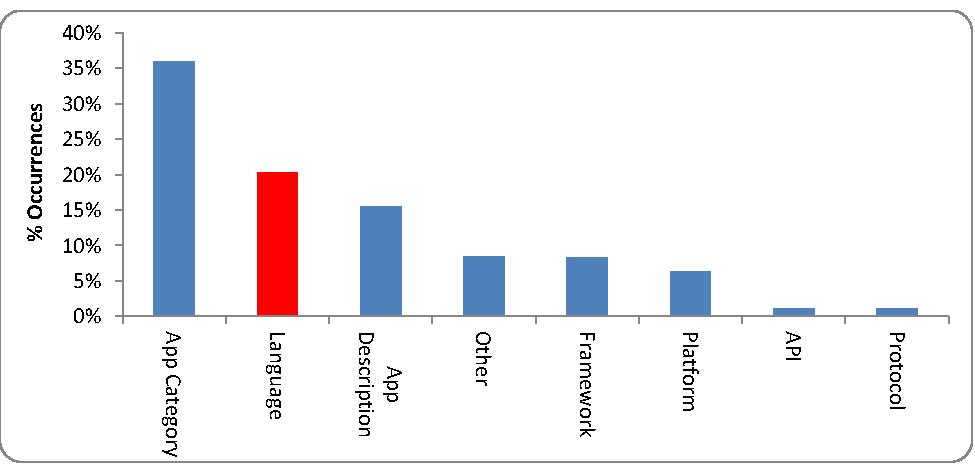
\includegraphics[width=1.0\textwidth]{ProjectCategorisation.pdf}
\caption{A representation of the categorisation of tags and their relative occurrences}
\label{fig:ProjectCategorisation}
\end{figure}

\begin{table}
\centering 
\captionof{table}{The top 5 tags within the language category showing the 'Java' tag the most popular of all.}
\begin{tabular}
 \centering 
 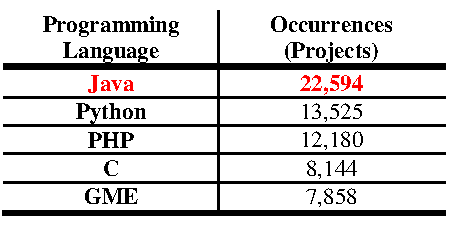
\includegraphics{GoogleCodeLanguage.pdf}
 \label{tab:GoogleCodeLanguage}
\end{tabular}
\end{table}

A \textit{sample} is extracted from the \textit{population} of 22,594 projects by iteratively invoking a simple pseudorandom function (the 'random' method in the Java Utils API which has an approximately uniform distribution) to select a number between 0-1 to be multiplied by the total number of projects available until the sample is extracted of an appropriate size. The selection algorithm discards from consideration any projects with no revision history as they represent projects which never saw committer activity beyond initial project creation and therefore have no relevance to this study. With a confidence level of 99\% and a confidence interval of 5\%, a minimum sample size of 646 was calculated. The actual sample size used was arbitrarily higher than the minimum sample size at 658 projects. 

Once the sample projects are selected, a utility in the toolchain allows for the automated parsing of the repository URL from the relevant project's page on the GoogleCode website. The project list with the associated URLs are then consolidated in a single file output which is used to drive the metric mining process.

\begin{table}
\centering 
\captionof{table}{The repository counts for each version control system.}
\begin{tabular}
 \centering 
 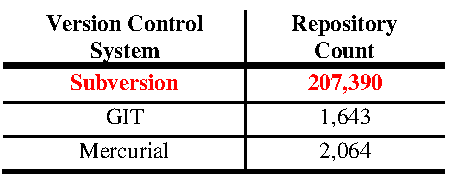
\includegraphics{GoogleCodeVCS.pdf}
 \label{tab:GoogleCodeVCS}
\end{tabular}
\end{table}


\subsection{Structural Metrics Mining}
The broad approach to mining project repositories for structural metrics is documented in section 3.3.6 of the previous chapter. This section builds upon that foundation to detail the aspects of mining that are specific to the particular analysis that forms the latter half of this chapter. For the initial univariate analysis, static code analysis is conducted on the latest version of the code of all selected projects within the sample. However, the later multivariate analysis, as will be covered in section 4.5, the identification of revision counts as a confounding factor will necessitate the analysis of every revision of each project and subsequently the static code analysis to mine for structural metrics - again for each revision. This creates a requirement to store structural metrics for each Java class file in each project for every revision of that project. Given that there can be hundreds of class files and thousands of revisions, this is a fairly large data set. In order to be able to query this data effectively there is a reliance on the database model documented in Figure ~\ref{fig:Schema}. This is in contrast to the univariate analysis where only a single set of structural metrics is captured for the entire project. Figure ~\ref{fig:AnalysisDataSets} illustrates the difference in these two approaches. On the left, there are three revisions and three classes: class A being revised three times and class C revised just once. On the right the contrast is shown between the univariate analysis (where only the final revision is considered) and the multivariate analysis (where all three revisions are considered).

\begin{figure}[htbp!] 
\centering    
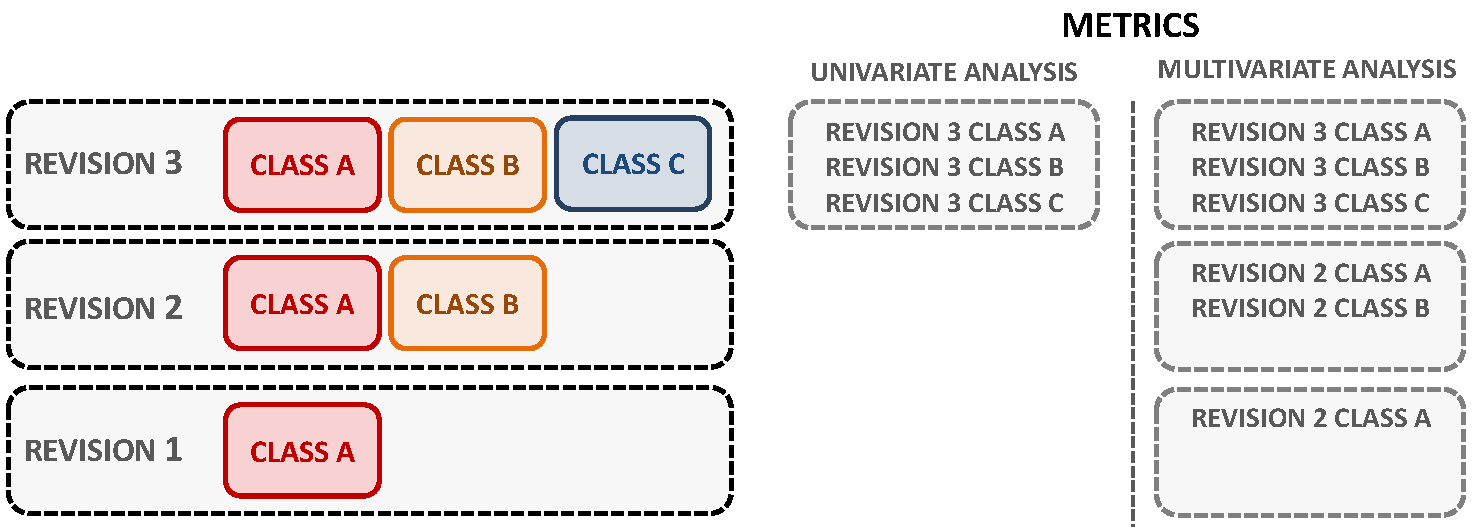
\includegraphics[width=1.0\textwidth]{AnalysisDataSets.pdf}
\caption{An illustration of the difference between data sets for each of the univariate and multivariate analysis.}
\label{fig:AnalysisDataSets}
\end{figure}

\section{Sample Analysis} %Section - 4.3 
Ahead of conducting a detailed analysis of the \textit{sample} or carrying out a regression analysis to answer the research questions, it is standard practice to conduct an initial exploratory data analysis. This is a typical approach in this type of research  \citep{grechanik2010empirical, cartwright2000empirical} as it enables for a dissection of the dataset allowing it to reveal its underlying structure without prior assumptions or biases. It is through that initial analysis that potential complexities or threats to validity can be identified mitigated \citep{tukey1977exploratory}. This section details that exploratory data analysis as applied to the \textit{sample} of 658 projects and presented against similar analysis in the \textit{population} of 22,594 projects. This analysis will show that the sample is broadly representative of the wider forge.

\subsection{Exploratory Data Analysis}
First, the extensions of files contained within the commits were mined and analysed with the results confirming a very heavy bias towards the Java file extension alongside other file extensions usually associated with Java web-based projects. This is as expected given the project sample selection criteria which exclusively selected 'Java' tagged projects. The results of this analysis are depicted in Table ~\ref{tab:GoogleCodeExtensions}. The table reveals a substantial proportion of XML files (typically used in Java projects  for configuration) and HTML and graphics files (mostly used in web-based projects).

\begin{table}
\centering 
\captionof{table}{File Extensions: top five cumulative occurrences.}
\begin{tabular}
 \centering 
 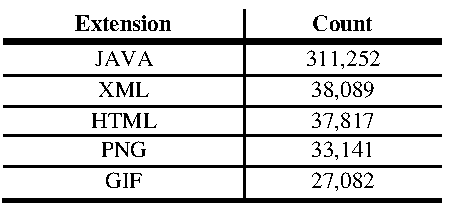
\includegraphics{GoogleCodeExtensions.pdf}
 \label{tab:GoogleCodeExtensions}
\end{tabular}
\end{table}

Next, the cumulative number of project committers was analysed. This is of relevance to this analysis as it is used as a measure of team size. Figure ~\ref{fig:CumulativeCommitterCount} shows that the sample follows a similar profile to the forge-wide analysis. Table ~\ref{tab:SampleTeamSizes} summarises the project team sizes in greater detail. The analysis reveals that more projects exist on lower committer counts; a fact that will have a bearing on the upper limit imposed on team size throughout the analysis in this chapter to help ensure a substantial population of data points for each team size that is included in this study.

\begin{figure}[htbp!] 
\centering    
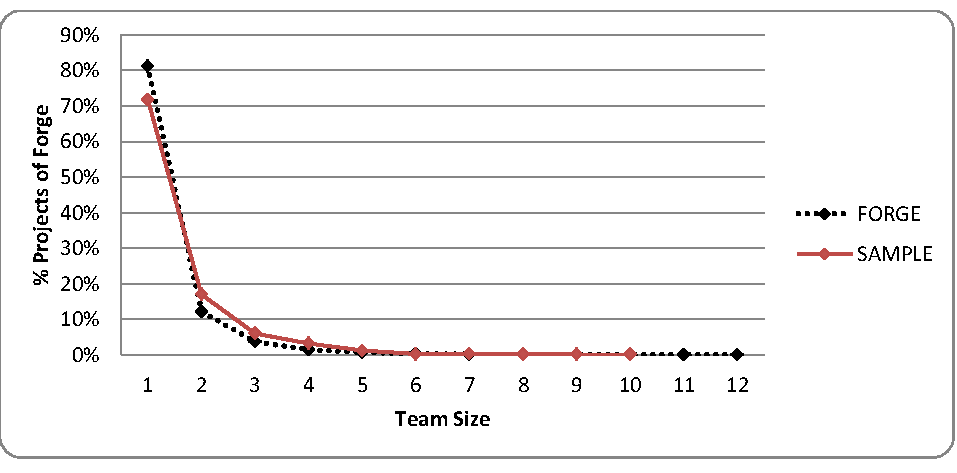
\includegraphics[width=1.0\textwidth]{CumulativeCommitterCount.pdf}
\caption{The number of projects with a team size of 1, 2, 3 through to 12.}
\label{fig:CumulativeCommitterCount}
\end{figure}

\begin{table}
\centering 
\captionof{table}{The number of projects within the sample of 658 projects, grouped by team size.}
\begin{tabular}
 \centering 
 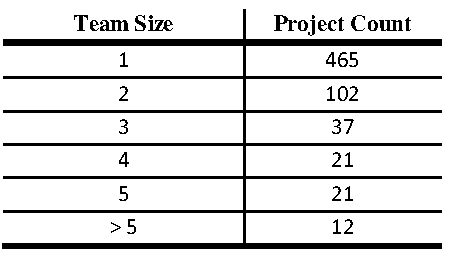
\includegraphics{SampleTeamSizes.pdf}
 \label{tab:SampleTeamSizes}
\end{tabular}
\end{table}

Committer behaviour was also analysed by investigating the cumulative number of commits grouped by committer and project, depicted in Figure ~\ref{fig:CommitCountBarChart}. It is notable that the broader forge shows a majority of committers only ever contributing a single commit when participating in a project. The sample deviates from this trend exhibiting a more even distribution across committer activity levels. This is attributable to the fact that the sample constituting only those projects tagged with the appropriate meta-data and, hence, are more likely to be active projects showing more sustained committer engagement. These trends will bear relevance to the multivariate team analysis later in this chapter where structural metrics are grouped by the number of revisions that files undergo.

\begin{figure}[htbp!] 
\centering    
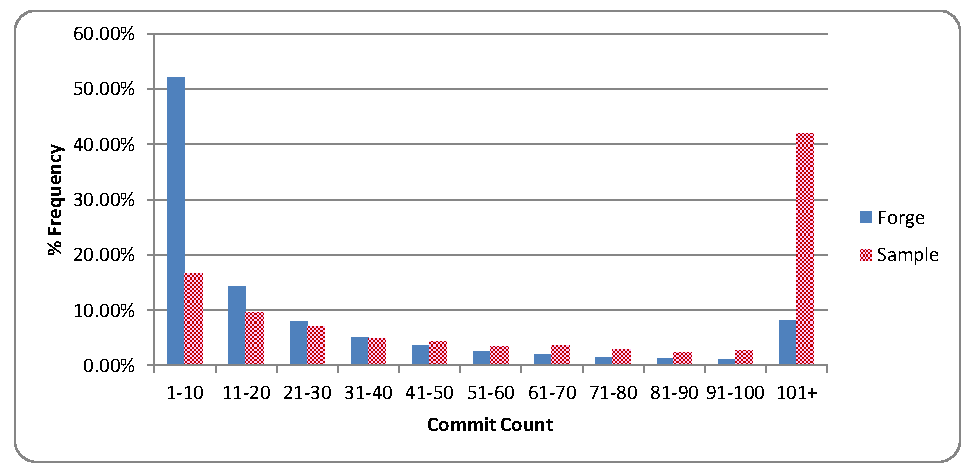
\includegraphics[width=1.0\textwidth]{CommitCountBarChart.pdf}
\caption[The number of commits that each committer makes within individual projects]{The number of commits that each committer makes within individual projects. The chart shows  x-axis shows the number of commits that a committer contributes to a project and the y-axis shows the frequency of that level of project engagement.}
\label{fig:CommitCountBarChart}
\end{figure}

The final aspect of sample analysis concerns the nature of the individual commits that make up committer activity. An individual commit can have any number of affected files. A commit could be a single file or path modification or, on the other extreme, the check-in of large mature codebase. Figure ~\ref{fig:AffectedFiles} shows the general trend that smaller commits are more frequent than larger ones. Any file-level analysis of commit information will necessitate the joining the structural metrics of potentially multiple affected files with the commit-level data. This will become apparent through the course of the multivariate team analysis.

\begin{figure}[htbp!] 
\centering    
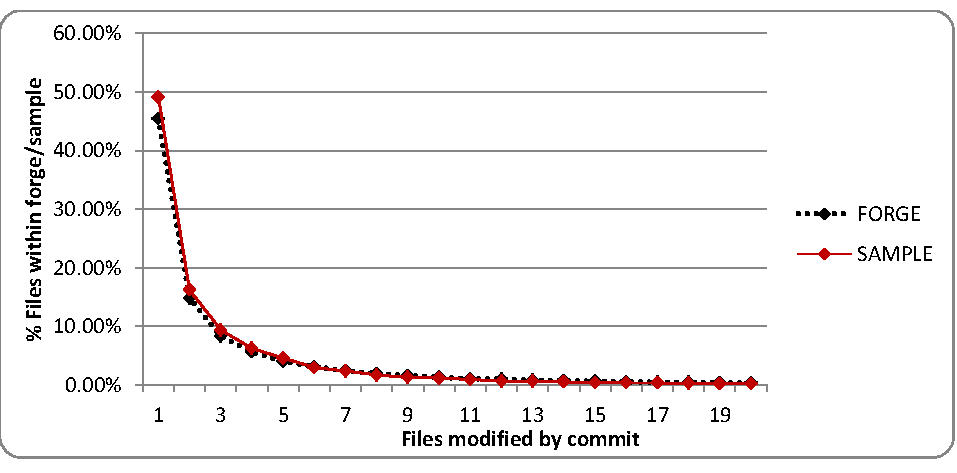
\includegraphics[width=1.0\textwidth]{AffectedFiles.pdf}
\caption{The frequency of commits grouped by the number of files affected.}
\label{fig:AffectedFiles}
\end{figure}

\subsection{Distributions and Correlations}
To conduct robust hypothesis testing and apply linear regression techniques, it is necessary to understand how the key parameters of the data set distribute relative to a normal distrubtion. An in-depth qualitative analysis of the distributions of CK metrics is not the focus of this work and the reader is referred to the work of Succi et al. \citep{succi2005empirical} and Basili et al. \citep{basili1996validation} for an analysis into the typical distribution of CK metrics for Java and C++ software respectively. For the purposes of this research the Kolmogorov-Smirnov test was used to compare the population of values of each CK metric against a normal distribution \citep{kolmogorov1933sulla, smirnov1948table}. This test makes no assumptions of the distribution of those data sets being compared and produces a p-value and a D-statistic as an output. Table ~\ref{tab:KSTest} shows zero p-values allowing the rejection of the null hypothesis of normality. The D-statistic indicates the ratio of the data sets that exists outside the normal distribution. This insight will influence the choice of statistical methods later in this thesis.

To analyse the relationship between the metrics within the sample, the Spearman correlation coefficients are analysed in Figure ~\ref{tab:MetricCorrelations}. The Spearman measure of correlation was chosen as it makes no assumptions of the normality of the distribution of the data being analysed \citep{spearman1904proof}. The correlation matrix shows positive correlations between CBO, LCOM, RFC and WMC. Weak correlations exist DIT, NOC and the remainder of the metrics. These observations are in-line with prior analysis by Succi et al. \citep{succi2005empirical}. Team size is found to be correlated to CBO and, to a lesser extent DIT, NOC and RFC. It is worth stressing that, for reasons explained in the next section, team size is measured at a project level while the metric values are at an individual class level. This initial result implies that greater team sizes cause metrics to trend counter to the objective as articulated by Rosenberg and others (detailed earlier in Chapter 2) - something which has been empirically associated with degraded external attributes. This adds further weight to the empirical evidence of prior research associating larger team sizes to lower productivity \citep{pendharkar2009relationship} and greater fault-proneness \citep{nagappan2008influence, caglayan2015merits}.

\begin{table}
\centering 
\captionof{table}{Results of Kolmogorov-Smirnov tests comparing the distribution of each metric against a 'reference' normal distribution.}
\begin{tabular}
 \centering 
 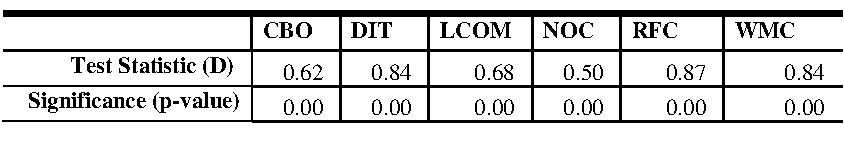
\includegraphics{KSTest.pdf}
 \label{tab:KSTest}
\end{tabular}
\end{table}

\begin{table}
\centering 
\captionof{table}{Spearman correlation matrix for Team Size and the CK metrics.}
\begin{tabular}
 \centering 
 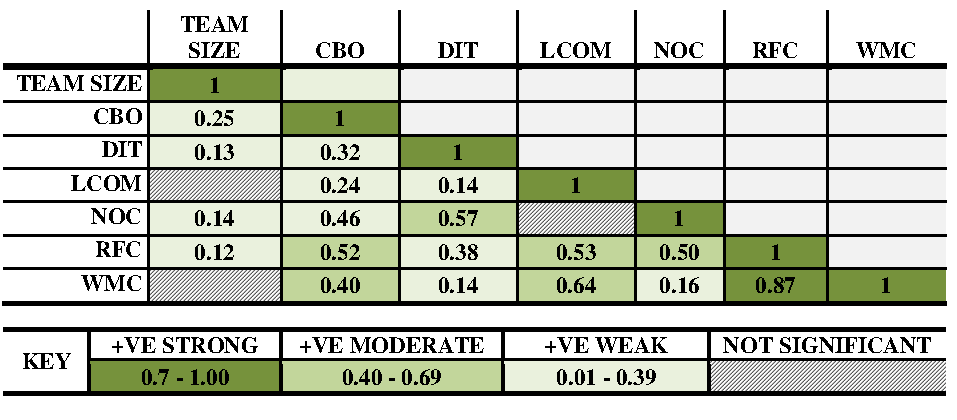
\includegraphics[width=1.0\textwidth]{MetricCorrelationsSpearman.pdf}
 \label{tab:MetricCorrelations}
\end{tabular}
\end{table}


\section{Univariate Team Size Analysis} %Section - 4.4
\subsection{Defining the Team Size}
For the purpose of this research, team size is defined as the cumulative total of all unique committers present in the revision history in the version control system of a given project. 

As alluded to in the previous section, while it is reasonable to suggest that such a definition would be an oversimplification as some committers could contribute to the codebase during widely varying time windows, it was posited that the majority do commit in overlapping time windows. This is borne out in analysis of the project sample that found that 83\% of committers to a project contribute in overlapping time windows to their fellow contributors, an example of which is shown in Figure ~\ref{fig:TeamSizeExample}. This fact, alluded to the reality that those committers who contribute outside the time window of their peers nevertheless leave an impact to the codebase which cannot be discounted, reinforces the argument in favour of a simple cumulative measure of team size.

Mockus et al. studied an Apache project and observed that the majority of development was attributable to a minority of 'core' developers \citep{mockus2000case} who commit frequently to the codebase. It could be suggested that the measure of team size proposed in this research does not distinguish between this frequent core committers and infrequent 'peripheral' committers. As Figure ~\ref{fig:CommitterCommitCount} illustrates, a significant amount of activity takes place by those committers who contribute with a low number of commits, hence infrequent committers cannot be excluded from any analysis without losing a key influencing factor on the codebase. Indeed Terceiro et al. studied the contributions of core and peripheral committers across 7 projects concluding that peripheral committers contribute a disproportionately high amount of structural complexity to the codebase further strengthening the argument that a measure of team size should include all committers \citep{terceiro2010empirical}. Figure ~\ref{fig:TeamSizeExample} highlights the simple and intuitive nature of a team size measure derived from the cumulative committer count as contrasted with a count of the number of committers with overlapping committer activity.

It is also reasonable to suggest that, given CK metrics are measured at an individual class level, so team size could also be measured at a class level (perhaps as the total number of committers to modify a class). This runs somewhat counter to the intention of making this research relevant to practitioners (particularly middle-management) which, the author argues, would relate much more to a measure of team size at a project level than at a class level.

\begin{figure}[htbp!] 
\centering    
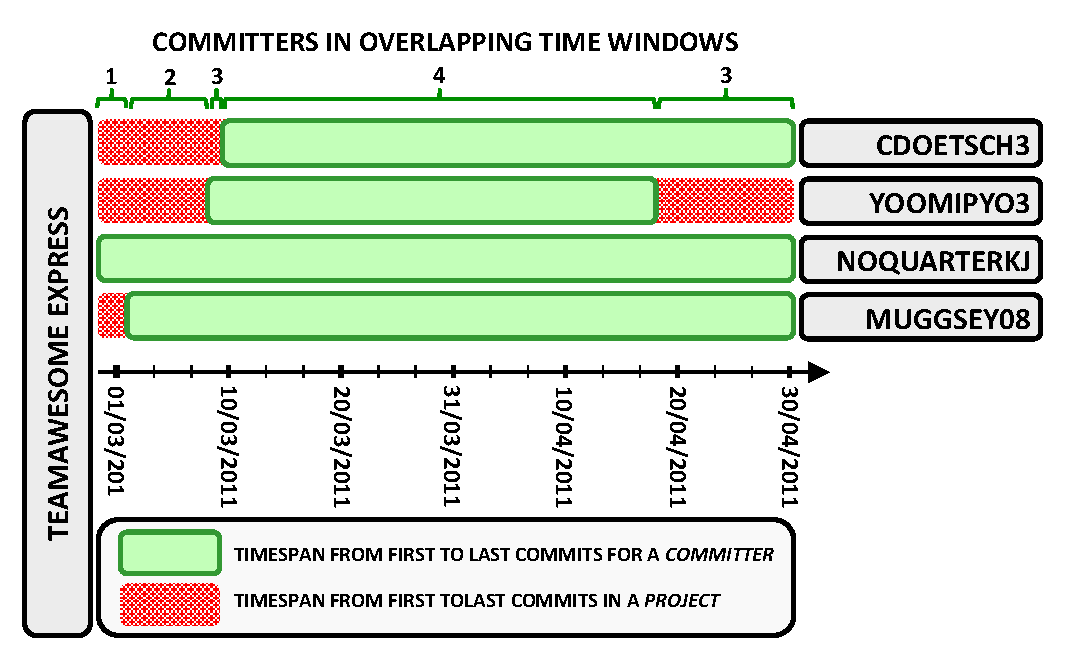
\includegraphics[width=1.0\textwidth]{TimeSizeExample.pdf}
\caption{The committer engagement timelines for project 'TeamAwesomeExpress'.}
\label{fig:TeamSizeExample}
\end{figure}

\begin{figure}[htbp!] 
\centering    
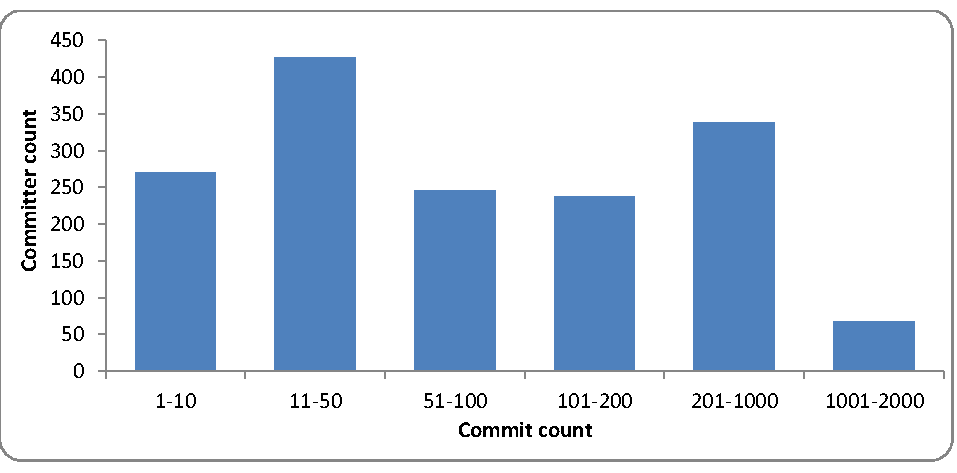
\includegraphics[width=1.0\textwidth]{CommitterCommitCount.pdf}
\caption{The number of commits that each committer makes within individual projects.}
\label{fig:CommitterCommitCount}
\end{figure}

\subsection{Analysis}
The analytical approach to the 'univariate' team size analysis uses, as its structural metric data set, the results of a static analysis of the projects codebases snapshotted at their final revisions. This is depicted in Figure ~\ref{fig:BasicAnalysisMetricMining} and illustrates the approach of overlooking the evolutionary path that a project took to reach its final (snapshotted) end state.

\begin{figure}[htbp!] 
\centering    
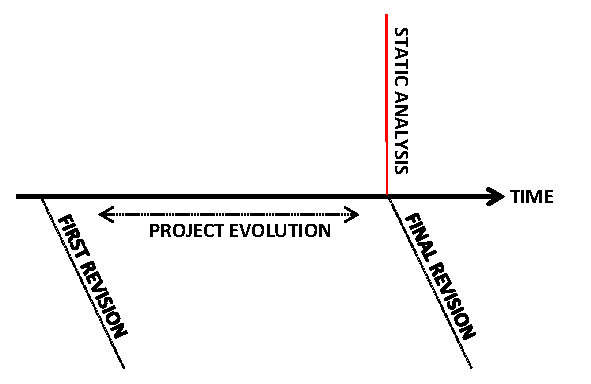
\includegraphics[width=0.7\textwidth]{BasicAnalysisMetricMining.pdf}
\caption{The evolution of project along the axis of time overlaid with a depiction of the point at which static analysis is conducted.}
\label{fig:BasicAnalysisMetricMining}
\end{figure}

Armed with these structural metrics, project metrics are then grouped or 'bucketed' according to the cumulative number of committers to the originating project. By way of example, should the total number of committers for a project number \textit{n}, then all the class-level structural metrics for that project would move into the \textit{n} committers bucket. This is illustrated in Figure ~\ref{fig:BasicBucketingStrategy}.
 
\begin{figure}[htbp!] 
\centering    
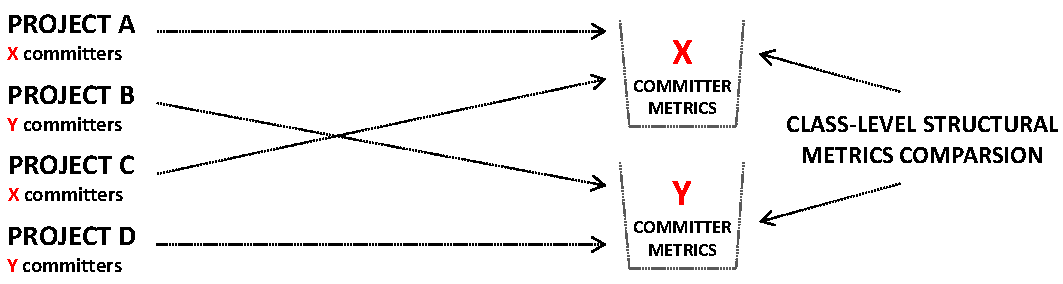
\includegraphics[width=1.0\textwidth]{BasicBucketingStrategy.pdf}
\caption{An illustration of our bucketing strategy categorizing the class-level structural metrics of a project according to the cumulative committer count of that project.}
\label{fig:BasicBucketingStrategy}
\end{figure}

As shown in the sample analysis in Figure ~\ref{fig:CumulativeCommitterCount} earlier, there is a dramatic drop in the proportion of projects that have a higher committer count compared with those projects with a lower committer count. In the sample this drop is particularly dramatic from 5 committers to 6 committers with counts of 12 and 3 projects respectively. For this reason, the statistical analysis excludes buckets for 6 or more committers. As will be discussed in Chapter 6, this can present an external threat to validity generalising some of the findings in this research to substantially larger team sizes. 

\begin{table}
\centering 
\caption{The bucketed metric comparison strategy.}
\begin{tabular}
 \centering 
 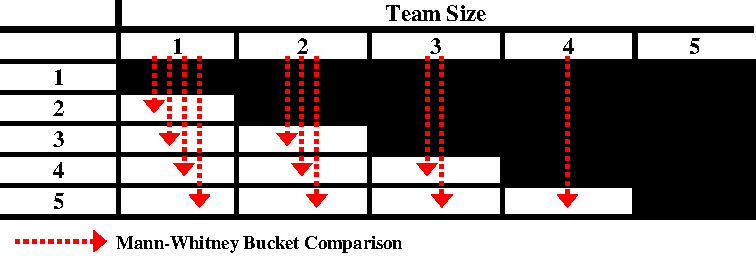
\includegraphics[width=1.0\textwidth]{MetricsComparisionStrategyTabular.pdf}
 \label{tab:MetricsComparisionStrategyTabular}
\end{tabular}
\end{table}

Table ~\ref{tab:MetricsComparisionStrategyTabular} illustrates the approach of comparing each bucket to every other. When comparing metrics populations bucketed by committer count, the Mann-Whitney test is ideally suited as all metrics populations are independent and consist of continuous non-normal data \citep{mann1947test}. Unlike the t-test, the Mann-Whitney test is a null hypothesis test that makes no assumptions of the distribution of the data. Null hypothesis H0,1 anticipates no significant difference between bucket populations of varying committer count and is rejected where the p-value is less than a certain threshold denoted by $\alpha$. With a target confidence level of 95\% this would imply a p-value cut-off ($\alpha$) at 0.05. However, a number of hypothesis tests are conducted, increasing the likelihood of observing at least one significant result at our chosen value of $\alpha$. It is therefore necessary to apply the 'Bonferroni correction' which sets the significance cut-off at the product of $\alpha$ and \textit{n} where \textit{n} represents the number of tests \citep{bonferroni1936teoria}. In this analysis there are 10 hypothesis tests for each metric giving a corrected $\alpha$ value of 0.005. Where the null hypothesis is rejected, the mean value of the bucketed metric populations are compared to determine in which direction the metric value is trending. Table ~\ref{tab:BasicResultsAverages} shows the mean metric value and observation count by bucket.

Table ~\ref{tab:BasicResultsSignificance} summarises the results of this analysis, based on which, two immediate observations can be made.

\begin{itemize}
\item  \textbf{Rejecting null hypothesis H0,1:} The null hypothesis can be rejected in the case of all metrics with the exception of NOC as p-values are lower than the  $\alpha$ for most of the remaining metrics comparison tests. NOC excepted, 44 out of 50 comparisons show p-values under the $\alpha$ threshold. 
\item  \textbf{Metrics not overwhelmingly trending in a one direction:} Based on the analysis of simple means, there is a roughly even split between metric values increasing in value by committer count and those decreasing in value. Looking at the trends in more detail, DIT and RFC bucket comparisons show a dominant trend of decreasing metric values with increasing committer count. However, DIT shows the opposing trend where 1 committer bucket is compared to 2, 3, and 4 committer buckets. Similarly, the LCOM bucket comparisons show a dominant trend of increasing metric values with increasing committer count.
\end{itemize}

While some trends do emerge from this analysis, it is important from the perspective of the validity of this research to ascertain whether there are any potentially confounding factors that may be impacting these results. That is the subject of the next section.

\begin{table}
\centering 
\captionof{table}{Tabular summary showing the results of each bucket comparison.}
\begin{tabular}
 \centering 
 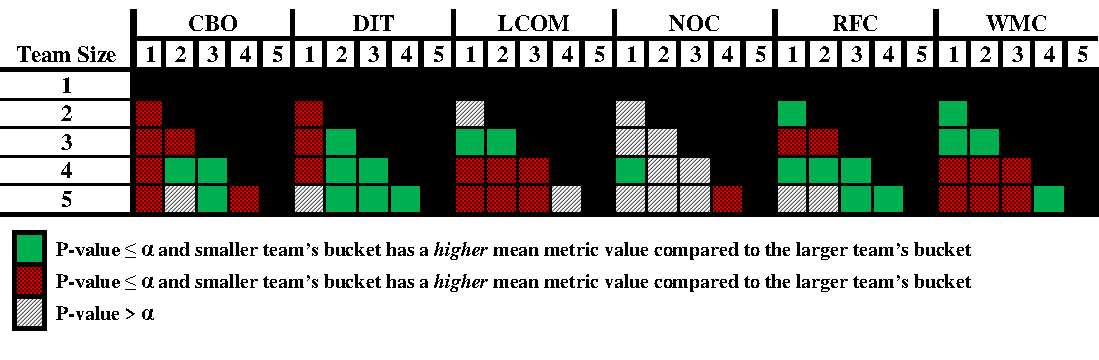
\includegraphics[width=1.0\textwidth]{BasicResultsSignificance.pdf}
 \label{tab:BasicResultsSignificance}
\end{tabular}
\end{table}

\begin{table}
\centering 
\captionof{table}{Metric mean values for each metric bucket.}
\begin{tabular}
 \centering 
 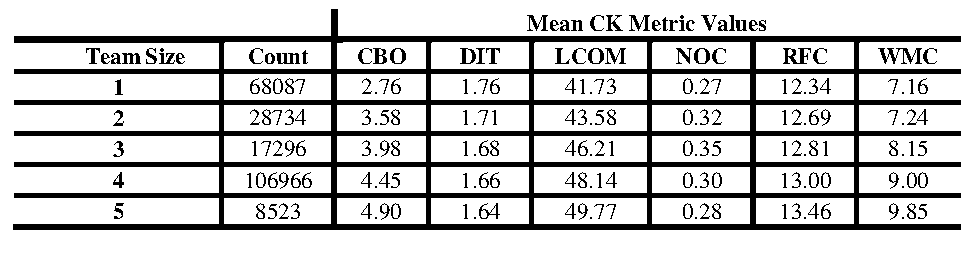
\includegraphics[width=1.0\textwidth]{BasicResultsAverages.pdf}
 \label{tab:BasicResultsAverages}
\end{tabular}
\end{table}

\subsection{Confounding Factors}
Confounding factors are those that influence both the dependent and independent variables within a model causing an association to be made which may not be genuine. In prior research modelling the impact of structural metrics on the externally observable attributes of software, class size was found to be one such factor. Emam et al. found that class size had a confounding impact on fault-proneness \citep{el2001prediction}. They suggested that earlier models which had established the predictive power of CK metrics over fault-proneness were largely (but not entirely) driven by class size and therefore not controlling for this confounding variable was a significant threat to validity. Their work was very recently corroborated by Gil and Lalouche \citep{gil2017correlation} who argued that this threat to validity also extends to other OO metrics. In a similar vein, Zhou and Leung found that class-size was a confounding variable to CK metrics models where change-proneness was the dependent variable \citep{zhou2006empirical}.

This research differs from the prior literature in that the CK metrics are essentially the dependent variables rather than the independent variables. For the purposes of the validity of this analysis, it is necessary to establish those factors that could potentially confound models that use CK metrics as the dependent variables.

\newline
\textbf{4.4.3.1 Class Size}
\newline
The typical measure of class size is  Lines of Code (or LOC). This is a simple measure of the number of lines within a class to the exclusion of comment lines \citep{nguyen2007sloc}. An analysis of the Spearman correlation p-values show no correlation between class-level LoC, team size and CK metrics. This is not surprising in an object-oriented language where one could reasonably hypothesise that a larger team is likely to work on a codebase which has more class files rather than larger class files per se. Similarly, LOC shows very weak negative correlations to the DIT and NOC metrics with almost no correlation to the rest of the metrics. On this basis it is accurate to say that class size has no relationship to either the dependent or independent variables in the model that was established in the previous section and therefore cannot be considered a confounding factor that should be controlled. Figure ~\ref{fig:AllMetricsAgainstLOC}  depicts how CK metrics trend against project size showing the mean metric values across individual projects against their aggregate Lines of Code (LOC) count. These charts show that at a project level there is no obvious relationship between code volume and metric values.

\begin{figure}[htbp!] 
\centering    
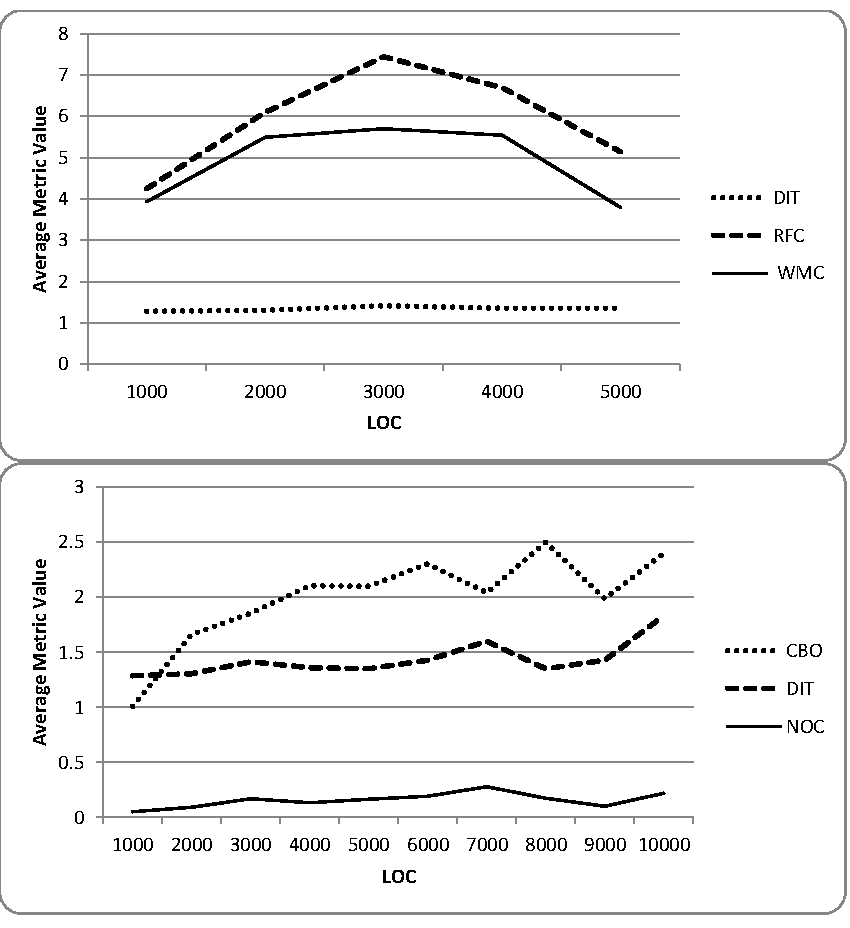
\includegraphics[width=1.0\textwidth]{AllMetricsAgainstLOC.pdf}
\caption{Mean project-level structural metric values plotted against the cumulative Lines of Code for that project.}
\label{fig:AllMetricsAgainstLOC}
\end{figure}

\newline
\textbf{4.4.3.2 Revision Counts}
\newline
When using version control systems, it is usual to build functionality iteratively through repeated modification of source files. This represents the development iterations driving the evolution of the codebase. It has been proven that, as software projects evolve, iterations of a codebase tend to exhibit both growing size and complexity \citep{prather1984axiomatic}. Each time a file (or group of files) is edited and re-committed this is considered a single revision. Revisions are tagged with commit comments which often refer explicitly to additional functionality that relates to the commit. An example of this can be seen in Figure ~\ref{fig:PreciseRevisionLogs} which is an excerpt from the revision logs from a project called 'Precise', a requirements management tool, which will be studied in more detail in a later chapter.

\begin{figure}[htbp!] 
\centering    
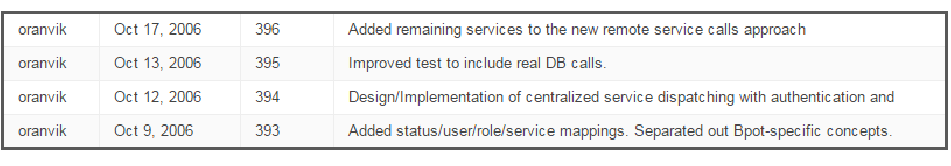
\includegraphics[width=1.0\textwidth]{PreciseRevisionLogs.pdf}
\caption{An excerpt of the revision log from the 'precise' project showing commentary explaining the addition of functional complexity with each revision.}
\label{fig:PreciseRevisionLogs}
\end{figure}

To date in this thesis, references to complexity have, in fact, alluded to structural complexity. This was defined earlier as the measure of the degree of interactions between components in a software system. This is in contrast to functional complexity which has no single definition but generally refers to the degree of sophistication in the logic encoded within a software system. Revision counts are an important factor to study as, this research argues, it represents a proxy to functional complexity (albeit a flawed one). While measuring structural complexity is a fairly straightforward task captured by RFC and WMC metrics (to make no mention of Halstead or McCabe's complexity metrics which are specifically designed for this purpose) capturing functional complexity is notoriously more difficult. Several measures have been proposed, generally with a tendency to conflate functional and structural complexity through attempts to track the nature of control structures within the source code or interactions between components. It is understandable that code inspection would be the default approach to measuring functional complexity as, where requirements are documented, they are often fragmented and therefore difficult interpret in an automated fashion. 

Revision counts cannot be considered a perfect proxy to functional complexity as revisions will not exclusively be associated with the addition of new logic. Refactoring activities and bug fixes both necessitate revisions which would not add to the functional complexity. The efficacy of revision counts as a proxy to functional complexity is beyond the scope of this work but, nonetheless, revision counts are an important factor worthy of further study for its potential confounding effect.

Table ~\ref{tab:RevisionCorrelations} shows the Spearman correlation coefficients for the relationship of revisions to team size and also CK metrics. It is notable that revisions do have a marked positive correlation to team size (0.47) as well as to the CK metrics; particularly CBO and RFC (0.29, 0.21 respectively). While these correlations are weak (under the arbitrary threshold of 0.40) they are nonetheless significant and imply a linear relationship between revisions and both the independent and dependent factors in our earlier model; namely team size and CK metrics respectively.

\begin{table}
\centering 
\captionof{table}{Spearman correlation coefficients for revisions against team size and each CK metric.}
\begin{tabular}
 \centering 
 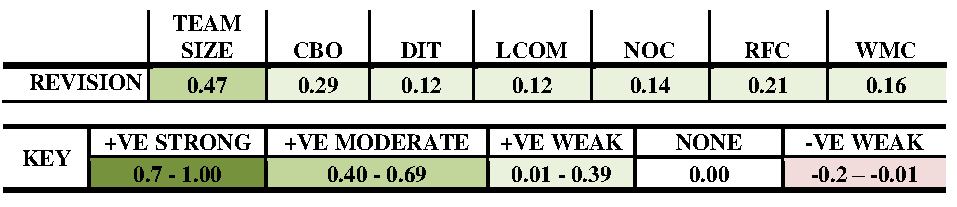
\includegraphics[width=1.0\textwidth]{RevisionCorrelationsSpearman.pdf}
 \label{tab:RevisionCorrelations}
\end{tabular}
\end{table}

This relationship between revisions and team size is confirmed at a project level with Figure ~\ref{fig:RevisionsCommitters} showing that the cumulative number of committers to a project trending positively against the number of revisions that the project has undergone. Furthermore, Figure ~\ref{fig:MetricsRevisions} demonstrates a clear positive correlation between class revision counts and all CK metrics with the exception of DIT and NOC. These metrics capture a very specific facet of structural complexity - inheritance complexity - which the results imply is not correlated with functional complexity. These results are consistent with the work of Johari et al. \citep{johari2012validation} who studied the relationship between CK metrics and revision counts on an open-source project. 

\begin{figure}[htbp!] 
\centering    
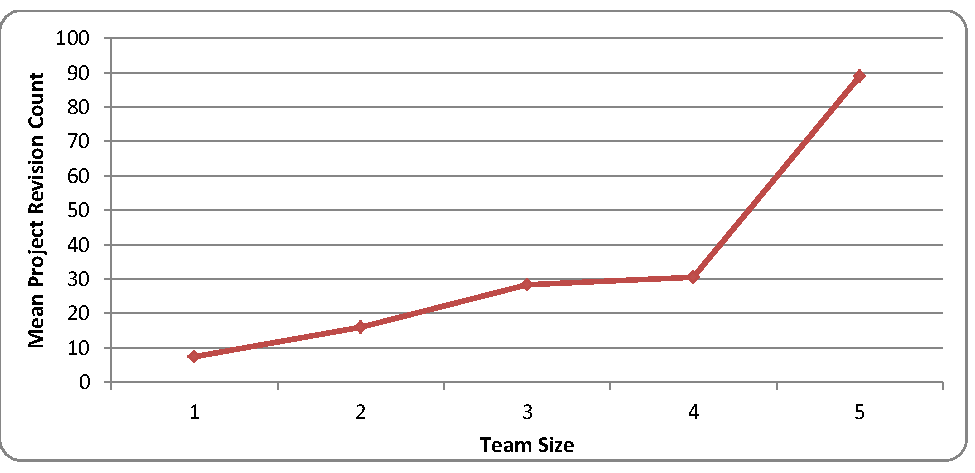
\includegraphics[width=1.0\textwidth]{RevisionsCommitters.pdf}
\caption{Analysis of the sample projects showing a clear upwards trend of the project revision count against committer count.}
\label{fig:RevisionsCommitters}
\end{figure}

\begin{figure}[htbp!] 
\centering    
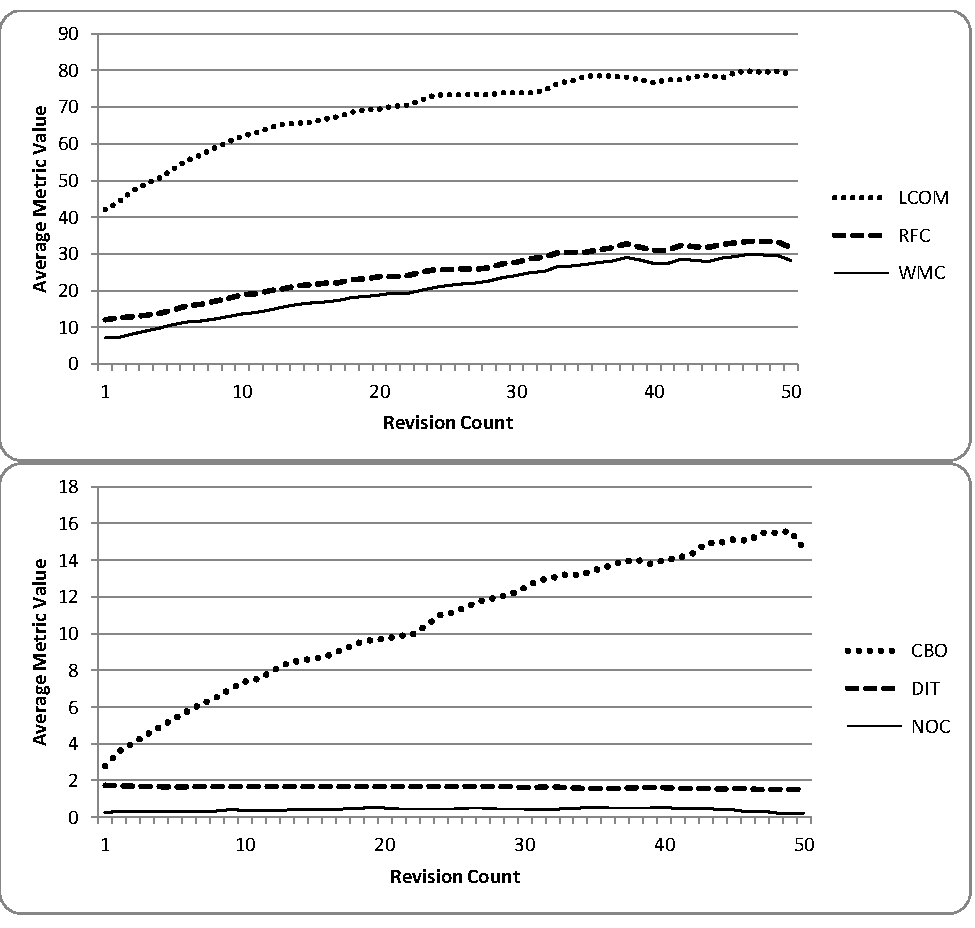
\includegraphics[width=1.0\textwidth]{MetricsRevisions.pdf}
\caption{Mean metric values at a class level plotted against the cumulative revision count of those files.}
\label{fig:MetricsRevisions}
\end{figure}

\section{Multivariate Team Size Analysis} %Section - 4.6

\subsection{Data Analysis Approach}
Having established revision counts as a confounding factor, in order to accurately study the impact of team size and produce reliable comparisons between metric populations of varying committer count it is necessary to control for revision counts. Continuing with the same sample as previously described, the data set takes the form of a class-level and revision-level CK metrics along with date and committer associated with each file revision as previously illustrated in ~\ref{fig:PreciseRevisionLogs}. This allows the determination of the number of unique committers to an individual project which is, as defined earlier, the project development team size. The approach of conducting static data analysis at each revision of the projects in our sample is illustrated in Figure ~\ref{fig:AdvancedAnalysisMetricMining}. This figure depicts the evolution of a project revised through its timeline of development with each revision the subject of static code analysis. 

\begin{figure}[htbp!] 
\centering    
\includegraphics[width=0.7\textwidth]{AdvancedAnalysisMetricMining.pdf}
\caption{Static analysis is conducted at each revision of the project evolution.}
\label{fig:AdvancedAnalysisMetricMining}
\end{figure}

Given this enriched data set, metrics can be grouped together by project team size - irrespective of the individual project from which they came - and considered distinct populations. For example, if project X and project Y each had the same number of unique committers, all metrics belonging to each file within both projects would reside in a single bucket. Using this bucketing approach, a set of distinct metrics populations can be compared using statistical techniques. From the meta-data associated with each file, the number of revisions any one file has undergone can be ascertained. This data will feed into the bucketing process where the population of metrics within a particular bucket only contains those metrics belonging to projects with a particular team size and only from files that have been modified a particular number of times. This approach, illustrated in Figure ~\ref{fig:AdvancedBucketingStrategy}, will give confidence that, when comparing our bucketed metric populations, any statistically significant differences are attributable to team size without the confounding impact of revisions.

\begin{figure}[htbp!] 
\centering    
\includegraphics[width=1.0\textwidth]{AdvancedBucketingStrategy.pdf}
\caption{An illustration of the bucketing approach used to categorise metrics for comparison.}
\label{fig:AdvancedBucketingStrategy}
\end{figure}
	
Consistent with the univariate team analysis in the previous section, as the dimensions in the data are not normally distributed, the Mann-Whitney test is again used to compare bucketed populations of metrics. Once again null hypothesis H0,1 is the subject of this analysis. H0,1 is rejected where the bucketed populations are found be independent where the p-values indicate a 95\% confidence level. As 50 hypothesis tests are executed for each metric, once again the Bonferroni correction need apply. This sets the p-value threshold of $\alpha$ at 0.001.

It is logical that there would be a greater number of metric results pertaining to the lower revision counts as, by necessity, for a file to be revised \texit{x} times, it would have \texit{x}-1 prior revisions (where \texit{x}>1). However, it is perfectly normal for a file to only have very few total revisions. This is an important consideration as those buckets with metric populations of higher revisions and committer counts have diminishing populations. Figure ~\ref{fig:MetricsPopulationRevisions} and table ~\ref{tab:BucketPopulations} show this effect. For this reason, and to ensure suitable metric populations in each bucket, in this analysis only buckets belonging to team up to 5 committers with a maximum of 6 revisions are considered. A substantial drop in bucket population is notable beyond these thresholds.

\begin{table}
\centering 
\captionof{table}{Bucket population sizes.}
\begin{tabular}
 \centering 
 \includegraphics[width=1.0\textwidth]{BucketPopulations.pdf}
 \label{tab:BucketPopulations}
\end{tabular}
\end{table}

\begin{figure}[htbp!] 
\centering    
\includegraphics[width=1.0\textwidth]{MetricsPopulationRevisions.pdf}
\caption{Mean metric values against revision count.}
\label{fig:MetricsPopulationRevisions}
\end{figure}

\subsection{Comparing Bucket Populations}
Table ~\ref{tab:ComplexResultsBucketComparisions} shows the results from the statistical tests run across each team-size comparison, similar to the previously discussed Table \ref{tab:BasicResultsSignificance} but also grouped by revision. By way of explanation, the first set of rows are bucket comparisons for the CBO metric. The revision columns relate to the number of times that the classes (from which the metrics were extracted to make the bucket metric populations) have been revised. The committer count columns and rows refer to the number of unique committers to the project from which the class originates. For completeness, those tests that do not meet the Bonferroni corrected $\alpha$ cut-off but do show significance at the 95\% confidence level are depicted accordingly. 

Where the bucket populations are found to be significantly independent the bucket population metric means are compared. Based on this, a determination is made as to whether increasing committer count will result in a rise or a fall in the metric value. The bucketed metric means are detailed in Table ~\ref{tab:ComplexResultsBucketAverages}.

From these results a number of notable observations can be made. 

\begin{itemize}
\item  \textbf{Rejecting null hypothesis H0,1:} After controlling for revisions it is still possible to reject null hypothesis H0,1 for all metrics but NOC and RFC. NOC showed no impact from team size before or after controlling for revision counts. However, RFC did earlier show a negative association with team size but this analysis has shown that this was due to the confounding impact of revision counts.  It is evident that a large number of buckets that show statistical significance across CBO, LCOM, WMC and, to a lesser extent, DIT.

\item  \textbf{DIT and LCOM show a positive relationship with team size at higher revisions:} The results for DIT and LCOM show a dominant trend of increased committer count resulting in increased metric values. In the case of DIT this trend is stronger at higher revisions of 4 and above. However, DIT does the opposing trend where 1 committer bucket is compared to 2, 3, and 4 committer buckets. Similarly, the LCOM bucket comparisons show a dominant trend of increasing metric values with increasing team size.

\item  \textbf{WMC shows a negative association with team size:} WMC shows a  trend with a decrease in metric value accompanying an increase in team size. 
\end{itemize}

\begin{table}
\centering 
\caption{Tabular summary showing the results of each bucket comparison.}
\begin{tabular}
 \centering 
 \includegraphics[width=1.0\textwidth]{ComplexResultsBucketComparisions.pdf}
 \label{tab:ComplexResultsBucketComparisions}
\end{tabular}
\end{table}

\begin{table}
\centering 
\caption{Metric mean values for each metric bucket}
\begin{tabular}
 \centering 
 \includegraphics[width=1.0\textwidth]{ComplexResultsBucketAverages.pdf}
 \label{tab:ComplexResultsBucketAverages}
\end{tabular}
\end{table}

\subsection{Simple Linear Models}
While the previous analysis focussed on holding revision counts constant, it is appropriate to model revision counts and committer counts as two independent variables with the CK metric values being their dependent variables, using simple linear regression to analyse their impact. Table ~\ref{tab:TeamSizeBasicLinearRegression} shows the output of this linear regression using the Ordinary Least Squares (OLS) regression method. One of the considerations when using this method for multivariate regression is that collinearity between the independent variables can lead to misleading coefficient estimates. The Variance Inflation Factor measures the increase of the variance of the parameter estimates if an additional variable is added to the linear regression. This helps ascertain the impact of collinearity of parameters on the validity of an OLS regression. At 1.65, this measure is significantly less than the 'rule of thumb' threshold of 5 \citep{menard2002applied}, hence the collinearity between revisions and team size is not a concern.

The linear models capture the linear relationship between team size, class revision count (as independent variables) and CK metrics (as dependent variables) expressed as the following equation where team size and revision count are multiplied by their respective coefficients $\beta$, $\gamma$ is the intercept, and $\epsilon$ is the standard error:

\[\large Metric \: Value = \beta_{TS}\, TS +  \beta_{R}\, rev +  \gamma + \epsilon \]

\begin{table}
\centering 
\captionof{table}{The results of an Ordinary Least Squares regression with committer and revision counts as independent variables.}
\begin{tabular}
 \centering 
 \includegraphics[width=1.0\textwidth]{BasicLinearRegression.pdf}
 \label{tab:TeamSizeBasicLinearRegression}
\end{tabular}
\end{table}

\textit{R-squared} is a statistical measure, ranging from '0' to '1', of how close the observed data points are to the fitted regression line. A value of '1' would imply that the independent variables linearly explain all variance of the respective CK metric.

The \textit{coefficients} are the estimated slope (that is to say the slope based on a sample of the population) of the component of the independent variable that is uncorrelated with the other independent variable. Coefficients cannot be directly compared across independent variables on the same model as they exist on different scales. For instance, if team size had the same impact on a metric value as revisions, it would still be expected that the coefficients of revisions would be lower given that they possess a higher range. Similarly it is not possible to directly compare coefficients of a specific independent variable across multiple CK metrics as here the dependent variables are on differing scales.

The \textit{residuals} are a measure of the distance between the actual observations and the model prediction. Table ~\ref{tab:TeamSizeBasicLinearRegression} shows the Root Mean Squared Error (RMSE) which is a measure of residuals in units of the respective CK metric. Residuals are difficult to interpret in isolation but will become useful when comparing the accuracy of these models against the mixed linear models in the next section.

The \textit{intercepts} are the values at which the fitted regression lines cross the y-axis. It is worth noting that the intercept point where team size and revisions are at '0' is purely a theoretical construct. It is useful, however, as it does indicate the degree to which the regression line is shifted upwards and will bear some relevance in Section 4.7 where intercepts of individual projects are compared.

\textit{Standard errors} indicate the degree to which the coefficient estimates may vary from the sample to the full population. This is a function of the \textit{R-squared} and the variance in the sample. \textit{T-statistics} are the ratio of the coefficient estimate and the standard error.  \textit{Degrees of freedom} are the number of independent observations available to establish a regression model.

The simple linear models detailed in Table ~\ref{tab:TeamSizeBasicLinearRegression} show a number of key results outlined as follows.

\begin{itemize}
\item  \textbf{Further rejection of null hypothesis H0,1:} In producing coefficients for team size and revisions, the linear modelling process first runs a hypothesis test to prove the rejection of the null hypothesis of coefficients of zero (i.e. the hypothesis that the independent variables have no effect on the dependent variables). This test returns highly significant p-values (approximated to 0.00) across all CK metrics.

\item  \textbf{Team size and revisions explain a substantial degree of variance, particular for DIT and LCOM:} It is notable that revisions and team size explain a substantial proportion of the variance in DIT and LCOM - 44\% and 43\% respectively - as represented by the R-squared values across the respective regression models. This is consistent with the results of the previous section that found that DIT and LCOM trended quite clearly positively with team size (controlling for revisions). NOC shows a R-squared value approximated to '0' which confirms the results of the spearman coefficient matrix that was presented earlier in Table ~\ref{tab:MetricCorrelationsSpearman} where no linear correlation was observed between NOC and the independent variables.

\item  \textbf{Inheritance complexity not impacted by revisions:} Coefficients close to zero for revisions across both DIT and NOC indicate that these metrics, both of which capture inheritance complexity, are not affected by revisions.

\item  \textbf{Team size trends positively with all CK metrics but NOC:} The positive estimated coefficients for team size ($\beta_{TS}$) across all regressions with the exception of NOC indicate that team size has a positive association with all but one of the CK metrics.

\item  \textbf{Low standard errors:} The standard errors indicate the probability that the sample mean and the population mean differ and therefore impact the estimated coefficients. The standard errors across the regression models do not rise above 0.03 indicating that, within a 97\% confidence level, the coefficients would prove accurate if calculated across the full population - i.e. all projects in the Forge.

\end{itemize}

\subsection{Linear Mixed Models}
While the application of the Ordinary Least Squares regression enabled the creation of some initial models, these models attempt to fit a single regression line per metric across the entire sample, disregarding the project-by-project variation. This is at odds with prior research which tends to produce a distinct population of observations for each project and study them individually using regression techniques (for the full survey refer to Tables ~\ref{tab:FaultModels} and ~\ref{tab:MaintainabilitySubatrributes}). This is somewhat intuitive as the idiosyncratic aspect of a project, driven by the nature and complexity of the functional behaviour as well as the individual programming traits of the individuals composing the team, has the potential to have a material impact on its structural metrics.

As this analysis is applied on a representative sample of an entire forge, it leads to a substantially larger data set than the 1-5 small/medium sized projects that is typical in the prior literature. As a result it is not feasible nor desirable to treat each project as an isolated data set as it would lead to a reduction in the degrees of freedom available to establish each individual linear model, consequently impacting the 'goodness of fit'.

Linear Mixed Models (LMMs) allow for a more nuanced linear regression by distinguishing between 'fixed effects' that apply to all groups and 'random effects' that apply individually to subgroups within data sets. Specifically, this approach can generate a single coefficient estimate but can allow for project-specific intercepts. This approach is useful in recognising and modelling the idiosyncratic 'project specific' impact to the metrics while using the full available data set to establish the coefficient estimates. 

This is the first application of LMMs to the study of software structural metrics but there is a substantial corpus of research that uses this technique in other fields. LMMs have gained recognition in the field of genomics for allowing 'relatedness' - modelled as the random effects - to factor in genetic association tests \citep{zhou2012genome}. Ecologists have recently started to apply this technique to modelling random effects of space, time and individuals in the study of species diversity and extinction risk \citep{bolker2009generalized}.

Linear mixed models can be expressed in a similar way to the previously specified OLS regressions in the previous section where $\gamma_p$ is now the \textit{project-specific} intercept:

\[\large Metric \: Value = \beta_{TS}\, TS +  \beta_{R}\, rev +  \gamma_p + \epsilon \]

Table ~\ref{tab:TeamSizeRandomInterceptsLinearRegression} summarises the results of a mixed model linear regression using project as the grouping variable. The coefficients and residuals are detailed as previously in the OLS regression results of Table ~\ref{tab:TeamSizeBasicLinearRegression}. The \textit{sample variance} shows the the degree to which observations are spread from the mean across the sample. The \textit{group variance} shows the same measure across individual groups and averaged across the full set of groups. This highlights the degree to which observations within a group share similar values when compared to ungrouped observations across the sample.

The following observations can be drawn from Table ~\ref{tab:TeamSizeRandomInterceptsLinearRegression}.

\begin{itemize}

\item  \textbf{Sample variance is substantially higher than group variance:} With the exception of the DIT regression, the groups exhibit lower variance than overall sample. This confirms that the  project-specific idiosyncratic characteristics have a significant bearing on metric values.

\item  \textbf{Lower Residuals:} The results from the LMMs exhibit substantially lower residuals across all metric regressions when compared to the OLS results in Table ~\ref{tab:TeamSizeBasicLinearRegression}. A reduction is expected as the intercepts are defined on a per project basis explicitly to reduce residuals.

\item  \textbf{Higher coefficient estimates:} The higher coefficient estimates in the LMMs indicate that team size and revisions have a greater impact on metric values than otherwise apparent in the OLS regression. While all projects share the same coefficient estimate, the revised values are attributable to the greater flexibility afforded by LMMs in fitting a regression line without forcing all projects through a single intercept.
\end{itemize}

\begin{table}
\centering 
\captionof{table}{The results of an mixed model linear regression with committer and revision counts as independent variables and the project as the grouping variable.}
\begin{tabular}
 \centering 
 \includegraphics[width=1.0\textwidth]{RandomInterceptsLinearRegression.pdf}
 \label{tab:TeamSizeRandomInterceptsLinearRegression}
\end{tabular}
\end{table}

\section{Results at a Project Level} %Section - 4.9
\subsection{Context}
While the analyses of the previous sections established a relationship between team size and CK metrics, it is informative to analyse individual projects at a code level and shed light on what may be driving the broader relationships observed. This section begins with the application of dimensionality reduction to visualise the team size sample which is then used to identify two individual projects for further study. Those projects are then analysed qualitatively through observing the source code of individual class files and quantitatively through metric values and LMM regression parameters.

\subsection{Project Selection}
To drive the process of project selection it is first necessary to visualise the project sample. This would enable us to ensure that the projects selected for study are not too similar but capture the diversity within the sample. Plotting a scatterplot for a data set with two dimensions is simple as the data can directly transpose onto the axis. When there are more dimensions the process of 'dimensionality reduction' can be applied. Principal Component Analysis (PCA) is one such technique, transforming the data set to a number of linearly uncorrelated dimensions \citep{pearson1901liii}. The 'Principal Components' are the combination of the original dimensions weighted to retaining the maximum variance within the data set.  PCA does not require the individual dimensions to be of any particular distribution \citep{timm10applied}.

Through the application of PCA it is possible to visualise the team size data sample through two orthogonal dimensions. This process results in 'loading coefficients' which weight each dimension within the sample to derive two principal components. As shown in Table ~\ref{tab:TeamSizePCA}, the first principal component is weighted towards CK metrics and particularly measures of structural complexity while the second principal component shows a greater bias to cohesion and team size.

\begin{table}
\captionof{table}{Loading coefficients of the Principal Component Analysis as applied to the team size analysis sample.}
\begin{tabular}
 \centering 
 \includegraphics[width=1.0\textwidth]{TeamSizePCA.pdf}
 \label{tab:TeamSizePCA}
\end{tabular}
\end{table}

Figure ~\ref{fig:TeamSizeScatter} shows a depiction of the team size sample scattered across these two principal components. No distinct clusters immediately emerge from this, but through this process it is possible to select two projects which are visually distant from one another for further study.

\begin{figure}[htbp!] 
\centering    
\includegraphics[width=1.0\textwidth]{TeamSizeScatter.pdf}
\caption{A visualisation of the team size sample scattered across the two principal components. The selection of Aviator and Precise for further study.}
\label{fig:TeamSizeScatter}
\end{figure}

Aviator and Precise are two projects that exhibit metric values that, relative to each other, are consistent with the wider forge trends for the given team sizes: one and five committers respectively. Aviator is located on the edge of the main cluster while Precise appears very much as an outlier - likely owing to its higher than mean LOC. Figure ~\ref{fig:TeamSizesResultsCompare} shows a comparison of the metric profiles between these two projects plotted against revision counts. Aviator is an expression engine that dynamically compiles expressions into Java byte-code and delivers them to a running JVM. It is a single committer project with the full codebase in Java and no graphical user interface. The project comprises 233 Java class files. The committer is currently a prolific contributor to open-source projects with an active public GitHub profile. The Aviator project represented one of his early efforts started after he had accumulated roughly 2 years of development experience. 

Precise is a requirements modelling and tracking tool designed to plug into the Eclipse IDE, with no dedicated user-interface as such. The project codebase comprises 524 Java class files alongside some modelling artefacts. Four distinct committers contributed to this project over a period of two years with the activity levels shown in ~\ref{fig:PreciseCommitterAnalysis}. It is notable that one committer contributes very little commits to the project while two committers contribute the majority of commits and unique files. The definition of team size within this research does not distinguish between the activity levels of committers in assigning a value to this measure. However, the final chapter of this thesis does consider avenues of future work to assess the impact to regression models by distinguishing between core and peripheral committers in the calculation of team size.

\subsection{Project Comparison}
Figure ~\ref{fig:TeamSizesResultsCompare} shows a comparison of the metric profiles between two projects plotted against revision counts. As previously, metric values are bucketed by revision count and averaged. It is notable that the observations for Precise are higher than those for Aviator for those metrics most affected by team size according to the linear regressions; CBO, DIT and LCOM. CBO and LCOM trend up with revisions, as expected given the positive coefficient estimates of the linear models. DIT does not exhibit a consistent trend against revision counts which is consistent with the earlier results which assigned a coefficient of zero to revision counts ($\beta_R$). 

\begin{figure}[htbp!] 
\centering    
\includegraphics[width=1.0\textwidth]{PreciseCommitterAnalysis.pdf}
\caption{Committer behaviour analysis for the Precise project.}
\label{fig:PreciseCommitterAnalysis}
\end{figure}

\begin{figure}[htbp!] 
\centering    
\includegraphics[width=1.0\textwidth]{TeamSizesResultsCompare.pdf}
\caption{Key structural attributes for the single contributor Aviator project compared against multi-contributor project Precise.}
\label{fig:TeamSizesResultsCompare}
\end{figure}

Within the Precise project there is some obvious fragmentation which can be observed through a fairly dis-organised source folder and package structure. Many classes are too large with 28 classes over 250 lines long, with code violating the 'single responsibility' principle which dictates that a class should do one thing and do it well. Failure to adhere to this leads to a lack of cohesion as member variables are rarely relevant to all methods in a fragmented class. Similarly a large number of methods would lead to a high values for WMC and CBO which are capture structural complexity and modularity respectively. To illustrate, Figure ~\ref{fig:BadCodeExample} shows a snippet of code from one of the most complex classes which contains 635 lines and 35 methods, most of which contain complex functionality. In one method there are seven nested conditional blocks, indicative of inordinate structural complexity and poor modularity. The revision history of this particular class shows that it had three distinct committers and had a high degree of structural complexity from the initial creation which steadily increased over subsequent revisions.
 
Precise has a significantly larger and more fragmented codebase than Aviator which appears to lead to fairly large class files with multiple responsibilities and points of coupling with other classes. By way of example, the ASMCodeGenerator class has responsibilities for code generation, arithmetic operations and maintaining complex collection structures indicating poor cohesion. Furthermore, as illustrated in ~\ref{fig:BadCouplingExample}, it directly coupled to multiple concrete implementations within the codebase, albeit mostly functionally oriented to code generation.  It is reasonable to postulate that a lack of effective coordination between committers on the Precise project lead, at least in part, to this fragmentation. This is a vicious cycle as poor structural attributes leads to further degradation as the codebase becomes more difficult to navigate and the demands for effective coordination between committers become unwieldly. All evidence is that the Precise project never made it to a fully-fledged release and ultimately failed as a project. Meanwhile Aviator continued to remain under active development after GoogleCode was decommissioned, migrating to GitHub and registering numerous releases.

\begin{figure}[htbp!] 
\centering    
\includegraphics[width=1.0\textwidth]{BadCouplingExample.pdf}
\caption{A depiction of the external dependencies to which the ASMCodeGenerator class is coupled.}
\label{fig:BadCouplingExample}
\end{figure}

\begin{figure}[htbp!] 
\centering    
\includegraphics[width=1.0\textwidth]{BadCodeExample.pdf}
\caption{A code snippet from the DomainProxyInvocationHandler class within the Precise project. The nested iterative blocks are numerically labelled.}
\label{fig:BadCodeExample}
\end{figure}

\begin{table}
\centering 
\captionof{table}{The intercepts and residuals for the Precise and Aviator projects.}
\begin{tabular}
 \centering 
 \includegraphics[width=1.0\textwidth]{RandomInterceptsLinearRegressionSelectedProjects.pdf}
 \label{tab:RandomInterceptsLinearRegressionSelectedProjects}
\end{tabular}
\end{table}

Table ~\ref{tab:TeamSizePCA} shows the intercept and residual values for the Precise and Aviator projects from the LMM regression in the previous section. The residual values of Aviator and Precise are consistent with their respective positions in the scatter plot. Precise, as an outlier in the scatter plot, could reasonably be expected to have a regression line that is compromised by the nature of the majority of the projects in the sample that make up the main cluster. This is reflected in higher residual values relative to the Aviator project. Conversely, the intercept values for the Precise project are significantly higher than Aviator. This is a result of the greater distance to the y-axis when extrapolating regression lines to achieve intercepts for projects with a higher team size. Given that projects with larger team sizes will have 'further to travel' in order to intercept with the y-axis, and that all projects will  have share a single gradient (the coefficient estimate) for a given metric regression, it is logical that those projects with a higher team sizes are likely to have lower (or even negative) intercepts. These observations help illustrate the strength of LMMs over OLS regression models within this context.

\section{Summary of Analysis} %Section - 4.7
To recap the analysis in this chapter, at the outset there was basic exploratory data analysis revealing underlying trends around committer behaviour and the nature of a commit as well as the distribution and correlations between the key variables in the data set. The analysis then moved on to tackling the first research question (RQ1) to establish if there was a relationship, at a forge level, between team size (the independent factor) and CK metrics (dependent factor). Then, following in the approach of the prior literature, there was a study of two factors for potential confounding impact, code size and revisions. It was determined that the former was not a confounding variable but the latter is. Revisions were then controlled for as a part of the next phase of analysis. The analysis to this point was achieved by taking observations from across projects and grouping them by team size and later by revisions, but always out of the context of the project from which they came. The latter section used the mixed models approach to linear regression to retain the project-specific idiosyncratic element to the data, re-evaluating the coefficient estimates and generate lower residuals. Finally the forge sample was visualised on a scatterplot, using PCA for dimensionality reduction, enabling the selection of two distinct projects for further qualitative and quantitative study. This helped shed light on the code-level features that drove the relationships reported by the linear models.

The results showed that projects developed by larger team sizes exhibited an increase in coupling (reflected by larger CBO values), an increase in inheritance complexity (reflected by higher DIT values) and a decrease in cohesion (reflected by larger LCOM values). This is a rejection of the null hypothesis H0,1 which anticipated no impact to any of the structural attributes of the software. Similarly, this leads us to accepting the alternate hypothesis H1,1.1, the basis of which was that prior research had linked larger teams to greater fault-proneness and, in the absence of further data, it was reasonable to hypothesise that maintainability and fault-proneness could be negatively correlated. There is consistency between the results of this team size analysis and the research of Nagappan et al. \citep{nagappan2008influence} who linked larger team sizes with increased fault-proneness given that Basili et al. had confirmed that CBO and DIT is highly correlated with fault-proneness \citep{basili1996validation}; this research having also observed higher CBO and DIT values from larger team sizes.

Referring to Table 2.5 (the survey of research correlating CK metrics to the sub-attributes of maintainability), inferences can be drawn from the observed structural trends against the impact on the maintainability of the software. Bruntink et al. had observed that DIT was negatively correlated with the testability while Badri et al. noted the same relationship between LCOM and testability \citep{bruntink2006empirical, badri2011empirical}. Harrison et al. found that LCOM was negatively correlated with changeability and Elish and Rine found that all CK metrics were negatively correlated with stability \citep{harrison1998investigation, elish2003investigation}.

Based on this prior research it can be deduced from the results of this chapter that the increased coupling, inheritance complexity and decreased cohesion of software associated with larger team sizes - represented by the higher values of CBO, DIT and LCOM respectively - result in degraded levels of the maintainability sub-attributes of testability, changeability and testability. This is an acceptance of alternate hypothesis H1,1.2 and is depicted in Figure ~\ref{fig:ResultOverview}.

\begin{figure}[htbp!] 
\centering    
\includegraphics[width=1.0\textwidth]{ResultOverview.pdf}
\caption[The impact of internal attributes on the maintainability of software.]{The impact of structural attributes on the maintainability of software. Coupling, cohesion and modularity and inheritance complexity all trend in a direction that indicates an attendant degradation in testability and stability and changeability.}
\label{fig:ResultOverview}
\end{figure} 
  
 \section{Chapter Review} %Section - 4.5
This chapter studied the relationship between development team size and the CK metrics of the produced software. This was done by first sampling the broader GoogleCode forge followed by exploratory data analysis studying committer behaviour and comparing the sample to the broader forge. Simple linear models were produced and the confounding factor of revision counts was identified. The multivariate analysis introduced revision counts into the linear model and, through studying individual projects in detail, the nature of the linear relationship was established.

The next chapter uses a similar approach to study the impact of team stability on the structural attributes of software. A distinction will be drawn between the team stability that is developed through the commit history of a project and the team stability that accrues across multiple projects.
%!TEX root = ../thesis.tex

\graphicspath{{Chapter5/Figures/}{Chapter5/Tables/}{Chapter5/Charts/}}

\chapter{The Impact of Team Stability on Structural Metrics}
\section{Introduction} %Section - 5.1 

The previous chapter focused on impact of team size on the structural metrics of software, addressing the first research question (RQ1). In this chapter, the focus turns to the second research question (RQ2);  \textit{the impact of the development team stability on the internal structural metrics of coupling, cohesion, complexity, and modularity of software projects and the implications on its maintainability}. Consistent with the previous chapter, a representative sample is first extracted and a measure of team stability is then presented. This is then used to drive a series of statistical analyses to answer the research question. At the outset of this chapter it is useful to restate the basic definition of team stability as the cumulative time that each team member has worked with their fellow team members. Consistent with the previous chapter, the definition of the team remains the set of unique
committers present in the revision history in the version control system of a given project. This initial basic definition of team stability will be developed and expanded upon through the course of this chapter.

Figure ~\ref{fig:chapter5overview} depicts the structure of this chapter starting with an initial treatment of those aspects of data mining and analysis that are foundational the team stability analysis which is detailed in the latter sections of this chapter. Section 5.2 outlines the approach to conducting network analysis throughout the GoogleCode forge; this is necessary to calculate a reliable measure of team stability. The pitfalls associated with forked projects and multiple committer identities are documented, along with mitigation strategies to these threats to validity. Section 5.3 is concerned with the second strand of foundational work - data mining and preliminary forge analysis to discover those basic trends that have a bearing on the latter analysis phase. Section 5.4 documents the approach to sample extraction necessary for the subsequent analysis in this chapter. Section 5.5 is a study of the impact of \textbf{'intra-project team stability'} on structural metrics; \textit{that is assessing how the stability accrued through the course of the evolution of the project affects its structural metrics, observing the project's final archived state within the forge}. Section 5.6 assesses the impact of \textbf{'inter-project team stability'} on structural metrics; \textit{that is the stability that is gained from retaining committers in a development team across multiple projects}. Inter-project team stability analysis factors in the chronology of projects and makes observations of the impact of stability that accrued in previous projects on structural metrics of the team's subsequent projects. Fortunately, given the breadth of the forge it is feasible to focus exclusively on the study of projects where an entire development team collaborated on a project and subsequently migrated, with the introduction of no new committers, to a later project. A comparison is carried out between the structural metrics of the chronologically earlier project against the later projects and, as in the previous chapter, functional complexity is isolated to remove any confounding impact it may have on the analysis. As in the previous chapter, section 5.7 presents the results in the context of two individual projects.

Figure ~\ref{fig:MiningAnalysisToolchain} highlights, at a high level, aspects of the toolchain that are of relevance to the team stability analysis - aspects that will be expanded on later in this chapter.

\begin{landscape}
\begin{figure}[htbp!] 
\centering    
\includegraphics[width=1.3\textwidth]{ChapterOverview.pdf}
\caption{Chapter 5 outline providing an overview of the contents of each section.}
\label{fig:chapter5overview}
\end{figure}
\end{landscape}

\begin{figure}[htbp!] 
\centering    
\includegraphics[width=1.0\textwidth]{MiningAnalysisToolchain.pdf}
\caption{Aspects of the toolchain pertinent to team stability analysis.}
\label{fig:MiningAnalysisToolchain}
\end{figure}

\section{Network Analysis} %Section - 5.2 
Network analysis is the process of mapping and measuring relationships between entities. This is a broad subject and there is substantial related work in the field of software development centred on project contributors as the entities to be mapped, usually focussing on studying communication between entities to understand the impact of various organisational dynamics \citep{martinez2008using, conaldi2013dual, daniel2016open, howison2006social}. This research is concerned with utilising network analysis techniques to make accurate observations of team stability that can then be used to drive comparisons between sets of structural metrics.

This research necessitates two types of network analyses illustrated in figure ~\ref{fig:NetworkAnalysis}. The first is a social network analysis focussed on committers where every single commit is mined and mapped to its respective project and the nature of the engagement of each committer's project engagement is analysed within the context of their fellow committers. This is used to calculate the stability of a team through the evolution of the project. 

The second type of network analysis - project-focused network analysis - is concerned with establishing the relationship of projects to one another. This relationship is given rise through the process of 'forking' creating, in essence, a dependency network. As will be discussed in this section, this relationship can distort analysis of committer history hence is it critical that this hierarchy is mapped out in order to eliminate this issue as a potential threat to validity. The project-focused network analysis in this chapter does not consider directionality although this will be discussed in the final chapter as a potential future avenue of work.

This section discusses each of these two types of network analyses separately, their associated mining challenge and the strategy to solve for those challenges.

\begin{figure}[htbp!] 
\centering    
\includegraphics[width=1.0\textwidth]{NetworkAnalysis.pdf}
\caption{A depiction of the network analysis conducted in the GoogleCode forge.}
\label{fig:NetworkAnalysis}
\end{figure}

\subsection{Committer-Focused Social Network Analysis}
The social network analysis strand of this research is concerned with mining the commit history of every committer in the forge, identifying which projects they contribute to, capturing the detail of their project engagement and analysing each committer's project engagement within the context of their fellow committers on those projects. The project engagement detail captured comprises the sub-modules that committers contribute to and the time interval of their contributions. This analysis will provide a basis for the calculation of intra-project team stability to be discussed in more detail in section 5.4.

A challenge to this network analysis is building the capability to consistently track committers as they traverse through the forge. When determining contributor activity, it is noted that multiple user identifiers are occasionally used by the same committer. Without rationalising these to a single identifier it is not possible to effectively track a committer's behaviour. As this research seeks to accurately establish the composition of development teams across all the projects in the forge in order to establish instances where groups of two or more committers contribute to more than one project together, it is essential to reliably identify committers across multiple projects. This is a common problem in the field of mining software repositories and has seen some earlier research efforts. Robles and Gonzalez-Barahona developed a methodology and general heuristics to identify developers across repositories (using data from VCS, mailing lists, and bug reports) \citep{robles2005developer}. They classify email addresses as a 'primary identity' which is almost always present across diverse repositories and they present a general approach to extract identities from email addresses. Applying this approach on the GoogleCode forge, it is observed that multiple email addresses can be attributed to the same identity.

To illustrate by way of example consider the two IDs below which, for the sake of this example, appear in the same project:

\textbf{ID1:} Jane Doe <jane.doe@doe.com> \\
\textbf{ID2:} Jane Doe <jdoe@doe.com>

Robles and Gonzalez-Barahona argue that it is a reasonable assumption that both these user handles refer to the same committer, albeit from two separate user accounts \citep{robles2005developer}. If this is not accounted for in the team stability analysis later in this chapter, this could result in an incorrect determination of the degree of stability attributed to a project.

Fortunately multiple user IDs for a single contributor usually carry sufficient similarity to allow automatic detection and rationalisation of these user IDs. Bird et al. propose a heuristic to rationalise user IDs when mining email social networks \citep{bird2006mining} which is partially adapted and adopted for this purpose. Specifically, there are several stages of name parsing that are applied:

\begin{itemize}
\item Where a name is accompanied by an email address in brackets the email address is ignored. In this case one user ID would be selected to which we assign the commits of both user IDs.
\item All names are converted to lower case and all trailing spaces are removed.
\item All punctuation is removed and replaced with a single space.
\item Multiple spaces are replaced with a single space.
\end{itemize}
 
When this type of network analysis is applied to the GoogleCode forge, it is observed that 17\% of unique committer identities are indeed sufficiently similar to be considered subtly different identities referring to the same committer. Naturally, activities on these alternate identities are conflated to represent a comprehensive view of the committer's behaviour.
 
\begin{figure}[htbp!] 
\centering    
\includegraphics[width=1.0\textwidth]{ProjectCommitterPrePostCleanup.pdf}
\caption{A depiction of the number of committers in the GoogleCode forge pre- and post-analysis.}
\label{fig:ProjectCommitterPrePostCleanup}
\end{figure}

\subsection{Project-Focused Network Analysis}
The project-focused network analysis within this research is concerned with mapping out the parent-fork relationships between projects. Forking refers to the process of creating an alternate and independent software development stream from an existing project. When unmapped, these relationships can pose a real threat to validity due to the duplication of commit history in the child project which can erroneously reflect those committers contributing to the parent project also contributing to the child project. This research seeks to study inter-project stability by studying projects where groups of committers genuinely contributed to multiple projects. Therefore this type of network analysis is necessary to avoid misattributing duplicated commits from forked projects to committers who have not genuinely contributed to those projects. 

\newline
\textbf{5.2.2.1 Mechanics of Forking}
\newline
One of the strengths of open-source software development is the ease with which one can start a new project leveraging all the tools that an open-source forge can offer. An unsuccessful project will attract few additional contributors while a successful project will build an active development community, produce artefacts and ultimately an active user base. Open-source forges also simplify the process of starting new projects based on the source code of existing projects and without affecting the original. The motivations to do so can range from discontent at the direction of development in the 'master' project through to a desire to build or experiment with new ideas within a mature project. The process of forking is named as such after the concept of forking processes to execute in parallel.

Forking projects can take multiple forms and each presents its own challenges in terms of automated detection. For the avoidance of doubt, when 'forking projects' are referred to, this is distinct to the 'fork and pull' development approach adopted by repositories such as GitHub, studied extensively by Kalliamvakou et al. \citep{kalliamvakou2014promises}. 'Fork and pull' is the process of cloning a master repository into an individual contributor's personal repository which acts as a staging area before changes, after review, can be merged into the master repository. This research, however, is concerned with forked projects that represent an entirely different development stream to the original project.

The process of creating a fork of a project can take several forms. This section discusses each approach illustrating using examples from GoogleCode.

\begin{itemize}
\item \textbf{Copying source files or binaries}
Some developers choose to fork projects by copying selected elements of the parent project's codebase. This could, for example, take the form of copying selected pre-compiled binaries or indeed the entirety of the source code. The example depicted in Figure ~\ref{fig:ForkedImportedBinaries} illustrates a snapshot of the revision history of the 'iTerm2' project - a MacOS Terminal replacement - which is a fork of the iTerm project. The second of the two revisions (r2) shows an import of the source files of the parent project. At the heart of this threat is that there is essentially no way of determining if a committer's contribution is their original work or whether it was fully or partially copied from other projects or sources without mining a host of other forges. While this is not a serious threat to the validity of this research, this could impact those researchers attempting to understand the value of developer contributions and would necessitate a mechanism to distinguish between a committer's original source code and that imported from other projects. For this reason, among others, development of techniques and software to identify 'code cloning' is an active field of research \citep{roy2009comparison}. While Brixtel et al. presented a framework which could be deployed for the purposes plagiarism detection \citep{brixtel2010language}, the majority of the efforts in this field focus on gaining greater understanding on the evolution of software repositories and reducing the wasted effort arising from duplicate code. Juergens et al. created an open-source workbench for code detection research geared towards configurability and extensibility and hence designed to support code clone research \citep{juergens2009clonedetective}. Lee et al. worked designed algorithms to support scalable indexing structures on vector abstractions of code to allow for the rapid detection of clones \citep{lee2010instant}. This work will be discussed towards the latter part of this thesis in the context of possible future work.

\begin{figure}[htbp!] 
\centering    
\includegraphics{ForkedImportedBinaries.pdf}
\caption{A snapshot of the start of the commit history of the 'iTerm2' project.}
\label{fig:ForkedImportedBinaries}
\end{figure}

\item \textbf{Cloning a repository within the forge}
Most popular version control systems make it fairly easy to clone a project, along with its full commit history into a new repository. Where this approach is taken to create a new fork, it will have an identical history to its parent. Figure ~\ref{fig:ForkedSameHistory}  shows the identical VCS history of the 'hotcakes' and 'zumastor' projects - both enterprise network storage solutions. In this example both projects share the same first 239 commits, after which they take divergent development paths. When conducting network analysis across the forge, without factoring in this threat to validity, it may be falsely observed that the committers of 'hotcakes' later contributed on 'zumastor'.

\begin{figure}[htbp!] 
\centering    
\includegraphics{ForkedSameHistory.pdf}
\caption{The identical VCS history of the 'hotcakes' and 'zumastor' projects.}
\label{fig:ForkedSameHistory}
\end{figure}

\item \textbf{Cloning a repository from outside forges}
This approach is a subtle variation on the previous method. Figure ~\ref{fig:ForkedOutsideForge} depicts the commit history of the 'cacheboy' project repository - a fork of 'squid' which is a webserver caching solution. Commits predate GoogleCode's launch by 9 years so clearly cannot be part of the 'cacheboy' project itself. These commits do, in-fact, belong to the 'squid' project which was hosted on a repository external to the GoogleCode forge. The existence of a parent outside the open-source forge will prove a challenge to detect. The threat to the validity of the network analysis in this case is the erroneous attribution of committer activity to a fork rather than a parent that resides outside the forge. This threat is of no consequence to this research given that the parent resides outside GoogleCode, there is no threat of 'double counting' the committer contribution; the risk is solely that the aggregate activity across the two projects is assigned to the later forked project. 
 
\begin{figure}[htbp!] 
\centering    
\includegraphics{ForkedOutsideForge.pdf}
\caption{The VCS history of CacheBoy.}
\label{fig:ForkedOutsideForge}
\end{figure}

\end{itemize}

\newline
\textbf{5.2.2.2 Identifying Forked Projects}
\newline
Identifying forked projects is an area which has seen some prior academic interest. Nyman and Mikkonen conducted research to establish the most common motivations for forking within SourceForge \citep{nyman2011fork}. The methodology to identify forked projects was to search the project descriptions that referred to forking. Although this approach suffices when attempting to locate a sample to study, relying on developers to specifically declare a project as 'forked' in the description does not help us identify a comprehensive set of forked projects to facilitate an accurate network analysis. Similarly, Robles et al. \citep{robles2012comprehensive} used a fairly manual approach for locating significant software forks that involved searching Wikipedia using the term 'software fork' and manually navigating to the project homepage to extract key information ahead of a study on the motivations and outcomes of forking. Again this cannot be applied to the large-scale mining of software forks within open-source forges making this approach inappropriate to identifying a comprehensive set of forks. 

As part of the process of maintaining a forked project, it is often desirable or indeed necessary to import changes from the master project. Ray and Kim developed a tool called REPERTOIRE to automate the identification of commonality between known forked projects through comparison of source files but it does not attempt identify forked projects in a wider open-source forge \citep{ray2012repertoire}. Of the approaches to automated clone detection, this is closest to the methodology adopted in this research. While REPERTOIRE tracks activity between known forked projects, this research is focussed on identifying the forked projects the co-exist within a forge. As such, this research can be considered complementary to the work of Ray and Kim.

This research proposes a heuristic which searches for common commits across projects and identifies them as projects exhibiting a fork relationship. Limitations to the heuristic tare outlined below.

\begin{itemize}
\item  \textbf{Coverage:} This approach is only capable of detecting forks where the parent also resides in the forge (or set of forges) being analysed; i.e. the mechanism of forking earlier referred to as 'cloning a repository within the forge'. This is not a limitation within the context of this research as this analysis is concerned with identifying those inter-project relationships that arise as a result of forking projects within the forge. This is because this forking mechanism was earlier identified at the only mechanism that has the capacity to create a distortion to the type of committer-focused network analysis conducted in this research. 
\item  \textbf{Forks by source file import:} As detailed earlier, some projects are forked by importing binaries and source files from other projects rather than importing the version control commits themselves. These forked projects are not detected by this heuristic but may be found by the other heuristics if the project or commit description contains the term �fork�. Again, this is not a limitation in the context of this work as these other forking mechanisms do not pose a threat to the validity of the network analysis in the latter parts of this chapter.
\item  \textbf{Context limitations:} This heuristic does not attempt to establish which, within a forking relationship, which project is the parent and which is the child. While establishing this relationship can be informative, as will be outlined in the Discussion chapter, it is not necessary for the purposes of the committer-focused network analysis in this research.
\end{itemize}

Figure ~\ref{fig:ForkCounts} shows the results of this analysis. 6.25\% of projects in the GoogleCode forge are forks of parent projects with a revision history that contains commits that are duplicated from the parent project. 

\begin{figure}[htbp!] 
\centering    
\includegraphics[width=1.0\textwidth]{ForkCounts.pdf}
\caption[A chart comparing the total number of active projects to the number of project forks.]{A chart comparing the total number of active projects (i.e. those projects with commits beyond the initial repository creation commit) to the number of project forks.}
\label{fig:ForkCounts}
\end{figure}

\section{Exploratory Data Analysis} %Section - 5.3
This section studies basic committer behaviour in order to analyse typical project engagement. This basic preliminary analysis will be valuable when conducting network analysis to calculate team stability.

Figure ~\ref{fig:LogCommitterCountProjectsEngaged} depicts the number of distinct projects that individual committers engage in, plotted against the log of the number of committers with that project engagement count. While 87\% of committers engage in a single project only, there are substantial numbers of committers that engage in multiple projects. This is significant as it indicates the availability of multiple committers engaging multiple projects - something that is critical for the identification of the inter-project team stability analysis data set as discussed in the next section.

Figure ~\ref{fig:FrequencyEngagement} is a representation of the duration of committer project engagement. This is calculated as the elapsed time (in units of days) between the first and last commits of individual committer on a project and is plotted against the frequency of that duration across all committer project engagements. It is observed that the majority of project engagements have a duration of eleven days or more. This has implications for the accumulation of intra-project team stability and, again, makes it likely that significant time overlaps between committers within a single project will be observed. As will be discussed later in this chapter, this is necessary for the accumulation of intra-project stability through the evolution of a project.

\begin{figure}[htbp!] 
\centering    
\includegraphics[width=1.0\textwidth]{LogCommitterCountProjectsEngaged.pdf}
\caption{The number of projects individual committers contribute to throughout GoogleCode.}
\label{fig:LogCommitterCountProjectsEngaged}
\end{figure}

\begin{figure}[htbp!] 
\centering    
\includegraphics[width=1.0\textwidth]{FrequencyEngagement.pdf}
\caption[The frequency of the timespan of project engagement.]{The frequency of the timespan of project engagement - measured as the time between the first and last commits on projects by individual committers.}
\label{fig:FrequencyEngagement}
\end{figure}


\section{Sampling} %Section - 5.4
The network analyses detailed earlier underpins the team stability analysis which is necessarily based on an accurate and comprehensive picture of committer project contributions and forge traversal. Where \textbf{intra}-project stability is studied, it is necessary to map the individual committer contributions at the project level. This type of analysis places limited demands on the requisite data set. Projects included in the data set should have more than one committer as there can be no meaningful analysis unless there are multiple committers. As with the team size analysis, it is possible to continue to restrict the study to Java projects only without unduly compromising the sample size. 

\textbf{Inter}-project stability analysis places greater demands on the data data-set and essentially should comprise pairs of projects where multiple committers migrate from a project, potentially shedding committers but not gaining any new ones, onto a new project. In order to provide contrast between the later project where committers have established some stability in comparison to the earlier project where the team stability would have been less, there should be no time overlap in the commit activity of the two projects. This criteria is illustrated in figure ~\ref{fig:ProjectPairEligability} below. The earlier project network analysis ensures that we reliably identify these project pairs without the distortion that forking can bring.

The network analysis discussed in section 5.2 enables the accurate and comprehensive mapping of committer project engagement throughout the forge. This facilitates the identification of projects where committers have contributed to more than one project alongside the same fellow contributors. This forms what is termed in this thesis a \textit{'stable partnership'}; i.e. two or more committers contributing to two or more of the same projects. This stable partnership is associated with a 'stable project pair'; this is to say that pair of projects where the 'stable partnership(s)' manifest. This is a simplification as there could be more than two projects where these partnerships appear. For the purposes of ascertaining the impact of stability this does not constitute a threat to validity, rather it is an opportunity for further work as will be discussed in the next chapter.

The expansive nature of the GoogleCode forge enables the application of fairly specific criteria to the identification of the inter-project analysis data set while retaining a statistically significant sample size. As illustrated in figure ~\ref{fig:ProjectPairEligability}, only project pairs where the commit history of the earlier of the projects concludes before the later project commences are included in the data set. This is to ensure that stable partnerships are captured rather than overlapping partnerships which could detract from the impact of the team's stability. Secondly, only those project pairs with committer populations entirely made of stable partnerships are eligible for inclusion; that is to say that the committers in the later project in the pair should be made up entirely of contributors from the earlier project. This is to avoid considering projects where the inter-project team stability is reduced by newcomers to the team. Finally, as discussed earlier in this chapter, the population sample must be cleansed of  forked projects with duplicated commit history as this is essentially distorted information which would constitute a threat to validity. 

\begin{figure}[htbp!] 
\centering    
\includegraphics[width=1.0\textwidth]{ProjectPairEligability.pdf}
\caption[An illustration of the 'project pairs' that are eligible for inclusion in the intra-project stability analysis.]{An illustration of the 'project pairs' that are eligible for inclusion in the intra-project stability analysis. While shedding team members from one project to the next is acceptable, additional committers is not. Projects must not overlap.}
\label{fig:ProjectPairEligability}
\end{figure}

This comprehensive criteria enables the creation of two distinct data-sets which can then be analysed relative to one another; projects where committers have previously partnered together 0 to \textit{n} times against those later projects where they have partnered 1 to \textit{n+1} times. By contrasting the structural metrics of each of the earlier projects within a stable project pair against the later project within that pair, it is possible to make some observations on the impact of team stability on these structural attributes of these projects.

For simplicity, once the data set for the inter-project stability analysis is identified, that same data set is leveraged to drive the intra-project stability analysis where projects are studied in isolation as opposed to within a their project pair.

The execution of this network analysis yields 508 project pairs - 1016 projects in total. Figure ~\ref{fig:ProjectCommitterCount} shows the committer counts across the sample, with the vast majority of projects exhibiting single digit committer counts. This trend is consistent with the observed trends in the forge analysis in the prior chapter as illustrated in figure ~\ref{fig:CumulativeCommitterCount}.

\begin{figure}[htbp!] 
\centering    
\includegraphics[width=1.0\textwidth]{ProjectCommitterCount.pdf}
\caption{Committer counts across the sample, with the vast majority of projects exhibiting single digit committer counts.}
\label{fig:ProjectCommitterCount}
\end{figure}

\section{Intra-project stability analysis} %Section - 5.4
The earlier definition of team stability - the cumulative time that each team member works with their fellow team members - is fairly broad and open to interpretation. This section provides greater precision around this definition and proposes a calculation for intra-project team stability - a measure capturing the degree of stability accrued by a team through the course of a project. 

\subsection{Determining a measure of intra-project stability}
This research proposes a measure of stability, assigned at a project-level, to capture the degree to which committers on a project accrue time working alongside their peers on the project. The premise of this measure relates to the earlier definition of stability from Huckman et al. which states that the greater cumulative time that a team of committers spend working with each other, the more stable that team \citep{huckman2009team}. 

Before delving into the specifics of how this measure is calculated, it is helpful to first explain that, within this model, there are two main constructs. The first is the 'time-frame of activity'. This applies both at level of the committer and the project and is defined as the window of time stretching from the first and last commits for that entity; specifically only those commits that impact Java source code, excluding for example, documentation changes. For instance, if a project records its first commit on the first day of January and it's final commit on the final day of December of that same year, it would have a time-frame of activity spanning the 365 days of that year. Likewise, a committer recording commits on the first and last day of January would have a time-frame of activity spanning the 31 days of that month.

\begin{figure}[htbp!]
\centering
\includegraphics[width=1.0\textwidth]{IntraprojectStabilityCalcOptions.pdf}
\caption{A hypothetical example showing three different approaches to calculating intra-project stability.}
\label{fig:IntraprojectStabilityCalcOptions}
\end{figure}

The second construct relates to how stability (or lack thereof) accrues on a project. Figure ~\ref{fig:IntraprojectStabilityCalcOptions} outlines three mechanisms through which a measure of stability can be derived. The first method (labelled '1') is the most straightforward and is to directly capture the number of days in each committers time-frame of activity through the course of the project. This is the most simplest transposition of the Huckman definition onto this problem space. However, it is also a measure that will closely track team size and does not capture the degree to which time-frames of activity overlap. The second method does capture the cumulative number of days that that these time-frames of activity overlap but will also be closely correlated with team size. The third method captures the extent to which the committer time-frames of activity \textit{do not align} with that of the project's time-frame of activity and therefore often misaligning with their peers and failing to accrue stability. For the reasons outlined below, this third method is chosen for this work and the measure is termed the 'Lack of Stability Ratio (LSR).

\begin{itemize}
\item  \textbf{Avoiding tracking team size:} As illustrated in Figure ~\ref{fig:IntraprojectStabilityCalcOptions}, the first two methods risk primarily tracking team size rather than stability. LSR, however, calculates a ratio which captures a particular aspect of committer time-frames of activity and therefore avoids tracking team size.
\item  \textbf{Adhere to conventions:} By measuring 'lack of stability' rather than 'stability', LSR continues the convention set by the CK metric suite and other software metric suites that favourable measures are lower in value (Lack of Cohesion being a pertinent example).
\end{itemize}

\subsection{Calculating LSR in practice}
An example of how LSR is calculated on a project from the stability project sample is illustrated in Figure ~\ref{fig:IntraprojectStabilityCalc}. The LSR calculation is based on the Jaccard Index where similarity is established between each and every committer time-frame of activity to the overall project time-frame of activity. 

The Jaccard index is the simplest of several similarity measures and was developed at the start of the previous century to compare botanical data sets \citep{jaccard1901distribution}. The Jaccard Index has some prior use in the field of mining software repositories. Kiefer et al. and Kpodjedo et al. use this measure to calculate similarity between Java classes to observe evolution of software projects through releases \citep{kiefer2007mining, kpodjedo2013studying}.  Jermakovics et al. used the measure to compute similarities among developers based on common file changes, constructing a network of collaborating developers \citep{jermakovics2011mining}.   Alternative similarity measures such as the S{\o}rensen-Dice coefficient \citep{sorensen1948method} or Euclidean distance add complexity but it isn't clear that either would better capture team stability given that they are more suited to weighting certain factors and clustering respectively. The Jaccard Index is defined as the size of the intersection divided by the size of the union of the sample sets.		

\newline
\[J(A,B)\ = \frac{\left |A\bigcap B \right |}{\left |A\bigcup   B\right |}\]

While the Jaccard Index is designed to establish the similarity between two finite data sets, the LSR calculation is an adaptation of this approach to take into account the fact that there can be more than two committer time-frames that need to be factored into the stability ratio. It is essential that LSR is in the form of a ratio to avoid calculating a number which has a strong direct correlation to committer count which would simply lead to tracking that factor and, ultimately, confounding results. As expressed in the equation below, LSR is the inverse of the simple averages of the Jaccard Indexes of each unique pair of committer time-series:

\newline
\newline
\[\large LSR \ = 1 - \frac{ \frac{Committer \mathit{1} \ \bigcap\ Committer\ \mathit{2}} {Committer\ \mathit{1}\ \bigcup\ Committer\ \mathit{2}} \ ...\ n } {n}\]

\begin{figure}[htbp!]
\centering
\includegraphics[width=1.0\textwidth]{IntraprojectStabilityCalc.pdf}
\caption{A worked example showing the calculation of the Lack of Stability Ratio (LSR) in a project called 'TeamAwesomeExpress' from the stability project sample.}
\label{fig:IntraprojectStabilityCalc}
\end{figure}

While the previous example is valid, it is also true that many software projects - particularly larger ones - are commonly divided into 'modules'; a fact that should be factored in the calculations. Each module represents a logical grouping of functionality with its source code typically residing in its own folder within the project repository. The concept of modules helps decouple sections of the codebase, providing the ability for specialisation amongst team members and reducing the need for coordination between them. Where the definition of team stability refers to team members 'working together', this should be expanded to stipulate that they work together on the same module, as otherwise there can be no assumptions on the degree of coordination between members - coordination being crucial to the accruing of stability in a team. 

Figure ~\ref{fig:ProjectModuleCount} shows the prevalence of multi-module projects throughout the stability analysis data set. Figure ~\ref{fig:IntraprojectStabilityCalcModularised} illustrates a worked example of a stability ratio calculation of a multi-module project.

\begin{figure}[htbp!] 
\centering    
\includegraphics[width=1.0\textwidth]{ProjectModuleCount.pdf}
\caption{The number of projects grouped by the number of distinct modules within their codebase.}
\label{fig:ProjectModuleCount}
\end{figure}

\begin{figure}[htbp!] 
\centering    
\includegraphics[width=1.0\textwidth]{IntraprojectStabilityCalcModularised.pdf}
\caption{A worked example showing the calculation of the Lack of Stability Ratio in a project called 'PipeDreamAgent' from the stability sample comprising two distinct modules.}
\label{fig:IntraprojectStabilityCalcModularised}
\end{figure}

\subsection{Validation of the Lack of Stability Ratio}
In the previous chapter, one of the key considerations was to mitigate for the fact that increasing team sizes can accompany an increase in functional complexity which could have a confounding impact. LSR is, perhaps, a less intuitive and direct measure than team size and, therefore, it is even more critical to quantify the relationship between this measure and other key factors that may have a confounding impact on CK metrics. Table ~\ref{tab:StabilityCorrelations} shows that LSR has negligible correlations to revision count, project duration and module count.

\begin{table}
\centering 
\caption{A matrix of Pearson correlation coefficients showing the relationship between various project-level variables}
\begin{tabular}
 \centering 
\includegraphics[width=1.0\textwidth]{StabilityCorrelations.pdf}
\label{tab:StabilityCorrelations}
\end{tabular}
\end{table}

By way of qualitative validation, it is notable in Figure ~\ref{fig:StabilityOutliers} that the visual representation of the time-frames of activity of two outlier projects from the stability sample show features that would be expected given their respective LSR values. The project named 'Dmdirc' has a high stability ratio and it is clear that the committers to this project work together for an extended period of time with an almost total degree of overlap. Conversely, 'Cykelgarage' shows an early commit by one author followed by a lull in activity and a series of commits by five other authors with some degree of overlap. While it is arguable that this measure inordinately penalises projects with an early commit followed by a period with no committer activity, it is also worth pointing out that this is quite a rare pattern and furthermore it is helpful to capture the gap in time that elapses between periods of activity as those gaps may be associated with a loss of knowledge from the team. In this particular example the commentary in the commit logs reveal that the initial commit activity to Cykelgarage represented an substantial check-in of code representing the first set of functionalities for the software. The subsequent lull is therefore significant in that it creates distance between the initial committer and the subsequent committers to the project - an aspect that is and should be captured by LSR.

The probability distribution for LSR across the stability project sample is illustrated in Figure ~\ref{fig:StabilityDistribution} and, while visually similar to a normal distribution, the Kolmogorov-Smirnov test returns a P-value of 0.00 and a D-statistic of 0.50 revealing that half the observations reside outside a normal distribution.

\begin{figure}[htbp!] 
\centering
\includegraphics[width=1.0\textwidth]{StabilityDistribution.pdf}
\caption{The probability distribution for the Lack of Stability Ratio (LSR) across the stability sample.}
\label{fig:StabilityDistribution}
\end{figure}

\begin{figure}[htbp!] 
\centering    
\includegraphics[width=1.0\textwidth]{StabilityOutliers.pdf}
\caption{Visualising the 'time-frames of activity' for two outlier projects; Cykelgarage and Dmdirc.}
\label{fig:StabilityOutliers}
\end{figure}

\subsection{Results}
The initial set of results visualisations are represented as scatter diagrams showing the average CK metric values at a project level plotted against LSR for those projects. Averaging CK metrics may be misleading as it can be heavily skewed by outlier values and thus misrepresentative of the data set. That said, it can be helpful as a first step in determining if there any clear trends manifest which can then be explored further. There are two observations that can immediately be made. First, the majority of the data points exist on the left-hand-side of the plots. This is a natural given that the majority of projects exhibit LSR values lower than 0.5 as confirmed by the probability distribution depicted in ~\ref{fig:StabilityDistribution}. The second observation is that there is no clear and powerful relationship between LSR and the project averaged metric values that manifest in these plots. 

\begin{figure}[htbp!] 
\centering    
\includegraphics[width=1.0\textwidth]{ScatterDiagrams.pdf}
\caption{Scatter diagrams plotting metric values against stability ratios.}
\label{fig:ScatterDiagrams}
\end{figure}

The charts in Figure ~\ref{fig:AverageMetricStability} average metric values for projects exhibiting a range of stability ratios. There is a noticeable upward trend across all metric types with the exception of CBO and NOC, implying at this early stage of analysis that teams with greater stability produce projects with higher cohesion and lower inheritance complexity. 

\begin{figure}[htbp!] 
\centering    
\includegraphics[width=1.0\textwidth]{AverageMetricStability.pdf}
\caption{Averaged project-level metrics grouped by stability ratio (rounded up to one decimal place).}
\label{fig:AverageMetricStability}
\end{figure}

Table ~\ref{tab:BasicLinearRegressionSingleFactor} shows the results of a basic Ordinary Least Squares linear regression with LSR as the sole independent variable. In a departure from the analysis in the prior chapter, it is not necessary to include revision count into this model as the correlation analysis in Table ~\ref{tab:StabilityCorrelations} shows that LSR does not track any of the key project-level factors and therefore those factors should not have a confounding impact. The model can be expressed as follows where LSR is multiplied by a coefficient ($\beta$), $\gamma$ is the intercept, and  $\epsilon$ is the standard error:

\[\large Metric \: Value = \beta_{LSR}\, LSR +  \gamma + \epsilon \]

A number of observations can be made based on the results in Table ~\ref{tab:BasicLinearRegressionSingleFactor}.

\begin{itemize}
\item  \textbf{Rejection of null hypothesis H0,2:} The R-Squared values show that LSR can explain a high proportion of the variance observed in the DIT and LCOM metrics, a substantial proportion of the variance of CBO, and a minimal element of the variance of RFC and WMC. All regressions report a p-value < 0.005 - i.e. the Bonferroni corrected $\alpha$ - and can be considered highly significant. CBO captures coupling and modularity, DIT captures inheritance complexity and LCOM captures coupling. Consequently, this model provides support for the alternative hypothesis H1,2.1 that \textit{'less stable development teams produce software exhibiting higher coupling, higher complexity, lower cohesion and lower modularity'}.

\item  \textbf{Stability has a powerful impact on CBO, DIT and LCOM:} The high coefficient estimates show that LSR has a fairly powerful impact on the CBO, DIT and LCOM metrics. For instance, the 8.67 coefficient reported in the CBO column indicates that a movement of 0.1 in LSR would have a 0.87 impact on the CBO; a metric with a mean of 3.55 within the stability sample. The low standard errors and high T-statistics show that this linear model provides a reasonable fit.
\end{itemize}

\begin{table}
\centering 
\captionof{table}{Results of the OLS linear regression with intra-project stability as a single independent variable.}
\begin{tabular}
 \centering 
 \includegraphics[width=1.0\textwidth]{BasicLinearRegressionSingleFactor.pdf}
 \label{tab:BasicLinearRegressionSingleFactor}
\end{tabular}
\end{table}

While this result evidences the impact of LSR on CK metrics, the 'idiosyncratic' project features referred to in Chapter 4 (previously established to play a significant role in the relationship between team size and CK metrics) is likely to play a role in determining how LSR impacts the structural attributes of individual projects. To take a hypothetical but intuitive example, if a software development team is geographically collocated and working on a highly complex problem, stability should have greater predictive power than for a development team that is geographically dispersed and working on a relatively simple problem solving to established and documented design patterns. While individually establishing the impact of these myriad of factors is well beyond the scope of this work, using the 'Linear Mixed Models' (LMM) statistical approach can, as demonstrated in Chapter 4, provide a linear regression which factors in this idiosyncratic component to establish coefficients with greater accuracy, reducing residual errors in the process. This can be expressed in a similar way to the equation in the previous section where $\gamma_p$ is now the project-specific intercept:

\[\large Metric \: Value = \beta_{LSR}\, LSR +  \gamma_p + \epsilon \]

Table ~\ref{tab:RandomInterceptsLinearRegressionSingleFactor} shows the results of the LMM regression and the following observations can be made. 

\begin{itemize}
\item  \textbf{Sample variance is substantially higher than group variance:} As observed with the LMM models of the previous chapter, the groups exhibit lower variance than the overall sample confirming the significant influence that the  project-specific idiosyncratic characteristics have on CK metric values.
\item  \textbf{Lower Residuals:} Again, consistent with the application of LMMs in the previous chapter, Table ~\ref{tab:RandomInterceptsLinearRegressionSingleFactor} shows substantially lower residuals across all metric regressions when compared to the OLS results in Table ~\ref{tab:BasicLinearRegressionSingleFactor}. 
\item  \textbf{Lower coefficient estimates:} The lower coefficient estimates in the LMMs indicate that team stability has less impact on metric values than otherwise apparent in the OLS regression. This is only noteworthy in the context of highlighting that LMMs revise the coefficient estimates to reduce residuals given the flexibility of project-specific intercepts.

\end{itemize}

\begin{table}
\centering 
\captionof{table}{Results of the 'random intercepts' linear regression with intra-project stability as a single categorical independent variable with observations grouped by project.}
\begin{tabular}
 \centering 
 \includegraphics[width=1.0\textwidth]{RandomInterceptsLinearRegressionSingleFactor.pdf}
 \label{tab:RandomInterceptsLinearRegressionSingleFactor}
\end{tabular}
\end{table}

\section{Inter-project stability analysis} %Section - 5.5
While studying intra-project stability enables the quantitative analysis of the impact of stability on the structural metrics of software, it is also informative to study at another key dimension of team stability; namely the impact of \textit{inter-project stability} on structural metrics; that is the stability that is gained through a development team retaining a consistent set of committers across multiple projects. This variant of stability intuitively can bear relevance to those practitioners looking to understand how continuing with an unchanged development team can bring benefits to internal and external attributes of the produced software. For this analysis the same null and alternate hypothesis hold as in the previous section; H0,2 and H1,2.1 respectively.

\subsection{Analysis approach}
As documented earlier in Section 5.4 of this chapter, there are a number of criteria that are applied in order to obtain a dataset that lends itself well to contrasting by inter-project team stability; namely that the project timelines should not overlap and that the chronologically later project should not contain any committers that did not exist in the earlier project. The nature of the subsequent analysis is twofold. First, the metrics of projects within 'stable project pairs' are compared to each other as depicted in Figure \ref{fig:StabilityAnalysis}. The second analysis is a linear regression to model the relationship between inter-project team stability and CK metrics.

To perform a linear regression, it is necessary to derive a categorical measure of lack of stability which can serve as an independent variable acting on CK metrics as dependent variables within the linear model. To achieve this the model assigns a binary with a value of '1' assigned to the first (chronologically) of a stable project pair and '0' assigned to the second project in the pair. This is an approach that attributes a total lack of team stability to the earlier project and total stability to the later project of the stable project pair. This is a simplification as it is entirely conceivable that any project team may have collaborated previously on other projects outside the GoogleCode forge and thus not captured within our data set and not reflected in this measure of lack of stability. Furthermore, in this analysis no account is made of the intra-project stability that accrues through the course of the earlier or the later project within a pair. These simplifications do not constitute a significant threat to the validity of this analysis as there is certainly an accumulation of inter-project stability from the earlier project to the later project within the stable project pair, enabling meaningful observations to be made. However, this measure leaves some scope for refinement as will be discussed in the Future Work in the next chapter of this thesis.

\begin{figure}[htbp!] 
\centering    
\includegraphics[width=1.0\textwidth]{StabilityAnalysis.pdf}
\caption{An illustration of the inter-project stability analysis approach.}
\label{fig:StabilityAnalysis}
\end{figure}

\subsection{Results}
Figure ~\ref{fig:InterprojectSignificance} shows the result of the first phase of analysis detailing the proportion of 'stable project pairs' where the structural metrics of the each member of the pair exhibit a significant difference from the other with a 95\% confidence interval; i.e. a Mann-Whitney test returning p-values of < 0.05. Significant difference across a large proportion of projects are observed - from a maximum of 38\% for RFC to a minimum of 22\% for NOC. Consistent with the inter-project stability analysis, this is further rejection of null hypothesis H0,2 that \textit{'Development team stability does not impact the coupling, complexity, cohesion or modularity of the produced software'}. The nature of this difference is studied, as in the prior analyses in this thesis, through linear modelling.

\begin{figure}[htbp!] 
\centering    
\includegraphics[width=1.0\textwidth]{InterprojectSignificance.pdf}
\caption{A chart showing the number of project pairs that show a significant difference (i.e. p-values < 0.05) between the metrics of each project in the pair. }
\label{fig:InterprojectSignificance}
\end{figure}

Table ~\ref{tab:BasicLinearRegressionInterprojectStability} details the results of an OLS linear regression with the categorical binary lack of stability measure as a single independent variable. Table ~\ref{tab:RandomInterceptsLinearRegressionInterproject} shows the results of the LMM Regression. The following observations can be made from these results.


\begin{itemize}
\item  \textbf{Further rejection of null hypothesis H0,2:} The R-squared values show that a substantial proportion of the DIT and LCOM metrics variance is explained by this inter-project lack of stability. The positive coefficients along with the low standard errors relative to those coefficients shows that CK metrics trend positively with inter-project lack of stability; a result consistent with the observations in the earlier intra-project stability analysis. This result provides further support for alternative hypothesis H1,2.1 that �less stable development teams produce software exhibiting higher coupling, higher complexity, lower cohesion and lower modularity�.

\item  \textbf{LMM results consistent with previous results:} When compared to the basic OLS regression, as with the intra-project analysis, the coefficient estimates are lower (with broadly lower residuals) given the project-specific intercepts of the LMM regression.
\end{itemize}

\begin{table}
\centering 
\captionof{table}{Results of the 'ordinary least squares' linear regression with inter-project stability as a single categorical independent variable.}
\begin{tabular}
 \centering 
 \includegraphics[width=1.0\textwidth]{BasicLinearRegressionInterprojectStability.pdf}
 \label{tab:BasicLinearRegressionInterprojectStability}
\end{tabular}
\end{table}

\begin{table}
\centering 
\captionof{table}{Results of the 'random intercepts' linear regression with inter-project stability as a single categorical independent variable with observations grouped by project.}
\begin{tabular}
 \centering 
 \includegraphics[width=1.0\textwidth]{RandomInterceptsLinearRegressionInterproject.pdf}
 \label{tab:RandomInterceptsLinearRegressionInterproject}
\end{tabular}
\end{table}


\section{Results at a Project Level} %Section - 5.7
\subsection{Project Selection}
Applying PCA to the team stability sample, a new set of loading coefficients emerge as documented in Table ~\ref{tab:TeamStabilityPCA}. It is notable that LSR hardly features in the first principal component. This can be explained by the fact that LSR explains a great deal of variance in the CK metrics - variance which is captured through the substantial loading coefficients on the CK metrics themselves. Figure ~\ref{fig:TeamStabilityScatter} shows the sample scattered by the two principal components.

\begin{table}
\captionof{table}{Loading coefficients of the Principal Component Analysis as applied to the team stability analysis sample.}
\begin{tabular}
 \centering 
 \includegraphics[width=1.0\textwidth]{TeamStabilityPCA.pdf}
 \label{tab:TeamStabilityPCA}
\end{tabular}
\end{table}

\begin{figure}[htbp!] 
\centering    
\includegraphics[width=1.0\textwidth]{TeamStabilityScatter.pdf}
\caption{A visualisation of the team size sample scattered across the two principal components. The selection of Aviator and Precise for further study.}
\label{fig:TeamStabilityScatter}
\end{figure}

Through the intra-team stability analysis, the broad trends observed were that DIT, LCOM, RFC, WMC trended positively with LSR. Two projects were selected with varying LSR values exhibiting relative metrics trends similar to those broader trends. Wikipedia-map-reduce and Scapi have LSR values of 0.41 and 0.15 respectively indicating that the latter has a project team which is substantially more stable. These particular projects were chosen as have similar revision counts (129 and 157 respectively) and five unique committers each. The two projects appear in distant positions from one another in Figure  ~\ref{fig:TeamStabilityScatter} with Scapi residing close to the center of the cluster while Wikipedia-map-reduce is very much an outlier owing to its high RFC and WMC values.

Wikipedia-map-reduce is an API that allows analysis of Wikipedia using the Hadoop Map-Reduce framework for parallel processing. Is is purely server-side software with no graphical interface. Scapi is a loan administration system which forms the basis of a company called Montep�o Plus which operates as an online pawn shop, swapping various personal items or assets for cash. 

Although both projects share the same team size, a deeper analysis of committer behaviour analysis depicted in Figure  ~\ref{fig:ScapiWikipediaMapReduceCommitterAnalysis} shows that Wikipedia-map-reduce has a single prolific contributor who is responsible for the majority of the codebase while Scapi's five committers more equitably distributed responsibility of the codebase amongst themselves. In the next chapter more consideration will be given to the role of 'core' committers versus that of 'peripheral' committers and how this can present both a threat to validity and an opportunity for further work.

\begin{figure}[htbp!] 
\centering    
\includegraphics[width=1.0\textwidth]{ScapiWikipediaMapReduceCommitterAnalysis.pdf}
\caption{Committer behaviour analysis for the Scapi and the Wikipedia-Map-Reduce projects.}
\label{fig:ScapiWikipediaMapReduceCommitterAnalysis}
\end{figure}

\begin{figure}[htbp!] 
\centering    
\includegraphics[width=1.0\textwidth]{TeamStabilityResultsCompare.pdf}
\caption{Key structural attributes for Wikipedia-map-reduce compared against Scapi.}
\label{fig:TeamStabilityResultsCompare}
\end{figure}

\subsection{Project Comparison}
Through qualitatively reviewing the code in both Scapi and Wikipedia-map-reduce, the latter emerges as the more structurally complex of the two projects. Although there is certainly less to critique in Wikipedia-map-reduce than in the previously reviewed Precise project - an observation which is consistent with the lower absolute LCOM and RFC numbers in Wikipedia-map-reduce relative to Precise - there are still some examples of poor encapsulation and inordinate structural complexity which will lead to poor cohesion, high coupling and low modularity. The Encoder class is an example of this as the code snippet in Figure ~\ref{fig:StabilityExample} highlights. It is an excessively large class at 1616 lines, 34 methods and four distinct inner classes. This class is fairly anomalous within the broader codebase which is generally well written.

In Wikipeda-map-reduce there is substantially more use of inheritance which confirms the higher DIT compared to Scapi (1.36 and 1.16 respectively). This is largely driven by the fact that Wikipedia-map-reduce has a substantial library of collections implementations which functionally lend themselves well to sharing behaviour via inheritance. 

Table  ~\ref{tab:RandomInterceptsSelectedProjects} documents the intercept and residual values for the Scapi and Wikipedia-map-reduce projects from the intra-project LMM regression. As was observed the similar analysis of team size in Chapter 4, the project that is more distant from the centre of the cluster exhibits higher residuals - in this case Wikipedia-map-reduce. This is attributable to the fact that the coefficient estimates of the regression line will be dominated by those non-outlier projects that make up the main cluster in the scatter plot and consequently show lower residuals. The intercept values are more difficult to interpret and are influenced by two key factors. The first is that Wikipedia-map-reduce has higher metric values which will influence a higher intercept value. However, given that the LSR is higher for this project, the regression line will have �further to travel� along the x-axis in order to intercept with the y-axis, which causes a decrease in the intercept values. As a result, the intercepts are a mixed bag with Wikipedia-map-reduce showing higher intercept values for CBO, DIT, NOC and RFC and lower intercept values for LCOM and WMC. 

\begin{table}
\centering 
\captionof{table}{The intercepts and residuals for the Scapi and Wikipedia-ma-reduce projects.}
\begin{tabular}
 \centering 
 \includegraphics[width=1.0\textwidth]{RandomInterceptsSelectedProjects.pdf}
 \label{tab:RandomInterceptsSelectedProjects}
\end{tabular}
\end{table}

While the team stability analysis has accurately identified project teams with a higher lack of stability  produces software with degraded structural attributes (from a maintainability standpoint), there are other influencing factors given that stability cannot explain all the variance in the structural metrics of the software. Of these project-specific 'idiosyncratic factors', such as relative experience levels or problem domain knowledge, further analysis would be beneficial but is beyond the scope of this work.

\begin{figure}[htbp!] 
\centering    
\includegraphics[width=1.0\textwidth]{StabilityExample.pdf}
\caption{A code snippet from Encoder class within the Wikipedia-map-reduce project. Multiple inner classes and nested iterative blocks are numerically labelled.}
\label{fig:StabilityExample}
\end{figure}

\section{Summary} %Section - 5.8
A number of observations can be made as a result of the analyses in this chapter. The intra-project stability analysis yielded clear trends with the introduction of the LSR measure being central to the analysis. Those teams accruing more stability throughout the project evolution exhibited structural metrics that tended to be lower across measures of structural complexity and cohesion. The trends on inter-project stability were similar. The approach of mining for 'stable project pairs' proved to be a useful approach in contrasting metric populations, showing significant difference between the structural metrics of the project pairs across a large proportion of the stability analysis data set. The linear regressions proved that a substantial portion of the variance with the sample was attributable to the categorical measure of lack of stability. However, the R-squared values were lower in comparison to the intra-project stability linear model, possibly attributable to the lower precision associated with the inter-project binary categorical lack of stability measure.

Given the negative correlation between these structural metrics and fault-proneness, it can be confirmed that the observations within this chapter are consistent with the work of Huckman et al. \citep{huckman2009team} and Gardner et al. \citep{gardner2012dynamically} who found that greater team stability was associated with lower fault-proneness. Referring, again, to table 2.4 (the survey of research correlating CK metrics to the sub-attributes of maintainability), inferences can be drawn from the observed structural trends against the impact on the maintainability of the software. With the results in this chapter showing that lack of cohesion, coupling and inheritance complexity tend to increase against a decreasing team stability, and given the already established negative correlations between the impacted CK metrics and maintainability in the prior art, it can be deduced that lower team stability leads to lower software maintainability. This is depicted in Figure ~\ref{fig:ResultOverview} and allows for a rejection of null hypothesis  H0,2 and a confirmation of the alternative hypotheses H1,2.1 and H1,2.2.

\begin{figure}[htbp!] 
\centering    
\includegraphics[width=1.0\textwidth]{ResultOverview.pdf}
\caption[Summary of the results of the Intra-project stability analysis.]{Summary of the results of the Intra-project stability analysis. This analysis shows similar trends to the team size analysis with Changability, Testability and Stability all associated with a degradation inline with the observed trends within the structural metrics.}
\label{fig:ResultOverview}
\end{figure} 
 

%!TEX root = ../thesis.tex

\graphicspath{{Chapter6/Figures/}{Chapter6/Tables/}{Chapter6/Charts/}}

\chapter{Discussion}
\section{Introduction} %Section - 6.1 
This chapter is organised into five sections as illustrated in Figure ~\ref{fig:chapter6overview}. Section 6.2 reviews the thesis objectives, hypotheses and research questions relative to the contribution of this research. Section 6.3 reviews the results of the analysis in detail through the prism of individual projects enabling a greater qualitative focus. Section 6.4 details the limitations of this work in the context of the threats that they pose to the validity of this research. Section 6.5 is a brief summary of the distilled conclusions of this thesis. Finally, section 6.6 documents future avenues of research within the field of mining software repositories.

\begin{landscape}
\begin{figure}[htbp!] 
\centering    
\includegraphics[width=1.3\textwidth]{ChapterOverview.pdf}
\caption{Chapter 6 outline providing an overview of the contents of each section.}
\label{fig:chapter6overview}
\end{figure}
\end{landscape}

\section{Objectives, Hypothesis, Research Questions Revisited} %Section - 6.2
In this section the objectives, hypotheses and research questions are reviewed, assessed and discussed relative
to the outcomes in the thesis.

Table ~\ref{tab:ObjectiveOutcome} shows a restatement of the objectives of this research assessed against the outcomes discussed in this thesis. Broadly the research objectives have been met and the results clearly show a relationship between the team factors and the internal and external attributes of the software. 

\begin{table}
\captionof{table}{Summary of objectives and outcomes.}
\begin{tabular}
 \centering 
 \includegraphics{ObjectiveOutcome.pdf}
 \label{tab:ObjectiveOutcome}
\end{tabular}
\end{table}

Table ~\ref{tab:HypothesisResult} summarises how the hypotheses formulated at the outset of this research mapped onto the results. The alternative hypotheses around the development team size analysis (H1,1.1, H1,1.2) stated that larger development teams would produce software with essentially degraded structural attributes resulting in degraded maintainability. The rationale of the hypothesis was based on the prior work of Nagappan, Caglayan et al, Mockus and Bell et al, all of whom observed that there was a negative correlation between development team size and fault-proneness \cite{nagappan2008influence}\cite{caglayan2015merits}\cite{mockus2010organizational}\cite{bell2013limited}. Given that fault-proneness and structural metrics are correlated, and in the absence of any code-level insights, it was considered a plausible hypothesis that all structural attributes of software and team size would show a similar correlation which would be indicative of lower maintainability. 

The results showed that those attributes that had been established to correlate to fault-proneness - coupling, cohesion, modularity - did, indeed, show degradation as team sizes increased. This was consistent with prior research and a confirmation of the alternative hypothesis. The drivers behind trends of degraded coupling and cohesion could be hypothesised to be attributable to the difficulties of effective communication in a larger team leading to developers with conflicting design patterns or alternate approaches causing degraded structural attributes. Through qualitative analysis and engaging development team members, the research community could shed more light as to the drivers behind the trends revealed in this study.

The alternative hypotheses (H1,2.1, H1,2.2) that less stable teams exhibit degraded structural metrics and lower maintainability was based on research by Huckman et al that found that greater team stability resulted in lower fault-proneness and higher budget adherence \cite{huckman2009team}. The rationale then followed, as with the previous alternative hypothesis (H1,1.1), that this was caused by a general degradation in the internal structural attributes of the software. Higher inter-team and intra-team stability was found to be linked to higher measures of cohesion and modularity, and lower measures of coupling and inheritence complexity. Again, through engaging development team members through surveys in conjunction with a detailed analysis of individual commits, further insights could be gained into the factors driving these observations.

\begin{table}
\captionof{table}{Summary of null hypotheses and results.}
\begin{tabular}
 \centering 
 \includegraphics{HypothesisResult.pdf}
 \label{tab:HypothesisResult}
\end{tabular}
\end{table}

Table ~\ref{tab:QuestionAnswer} summaries the headline results against each of the research questions. Broadly speaking, smaller development team sizes and greater team stability result in software with enhanced structural attributes. However, larger team sizes were found to be linked to lower functional complexity which is also associated with enhanced maintainability.

\begin{table}
\captionof{table}{Summary of research questions and answers.}
\begin{tabular}
 \centering 
 \includegraphics{QuestionAnswer.pdf}
 \label{tab:QuestionAnswer}
\end{tabular}
\end{table}

\section{Thesis Contributions} %Section - 6.X
The contributions in this work span three broad areas; furthering the art in the field of mining software repositories, the unique aspects of the linear modelling approach in this thesis and, finally, insights into the impact of team factors on the structural attributes of software.

\subsection{Open Source Forge Analysis}
As discussed in the Related Work chapter, the practical challenges of mining open source forges is well documented in existing research. Thematically this work covers tooling, pitfalls and insights from the perspective of researchers. Separately to this there is work that performs static analysis on selected open source projects and, also, extracts insights which can help process improvement in some fashion. This research focuses on a single open source forge and spans both of these areas of research with several specific contributions.

\begin{itemize}
\item  \textbf{GoogleCode forge  analysis: } This research studies an entire forge revealing several insights which go to a greater level of granularity than existing open source forge research which tends to derive insights at the forge and project level \cite{squire2017lives} \cite{howison2009flossmole} \cite{iqbal2012integrating}. Committer behaviour across the forge was studied as it informed the approach to the team size and stability analysis. It was possible, through this, to establish the population of unique committers (identity reconcillation challenges notwithstanding as documented in section 5.2.1) and track their activity throughout the history of the forge. This enabled observations on the number of projects that committers contribute to as well as the nature of their contributions (number of commits, number of files per commit and timeframes of activity). With this information it was possible to identify where committers collaborated on multiple projects, crucial to the team stability sample identification. This was a one of many potential use-cases for this type of data set and social network analysis in open source is an active field of research with plenty of other use-cases \cite{hassan2008road}\cite{hemmati2013msr}. For a representative sample of the forge it was then possible to mine structural metrics and join those observations to the commit meta-data (through the definition of a relational database schema). Through studying a observations from 173,190 class files in the team size sample it was confirmed that CK metrics from projects of this forge follow heavily skewed non-normal distributions in-line with the work of Succi et al \cite{succi2005empirical} and Basili et al \cite{basili1996validation} who had conducted their research on a smaller disparate data sets. The moderate collinearity between each of CBO (capturing cohesion and modularity) RFC and WMC (capturing structural complexity) was also confirmed.

\item  \textbf{Identifying forked projects: } Forking presents a number of perils when not properly considered. These perils can affect researchers extracting insights by mining version control system (VCS) histories, developers identifying projects to contribute to and end-users looking to utilise a project artifact. This research is concerned with the first use-case and has, for the first time, highlighted forking as a threat to the validity of network analysis in open source forges. Existing research focusses on project forking for the purposes of studying the its motivations and outcomes \cite{robles2006mining} \cite{nyman2011fork}. This reseach presents an approach to the automated identification of forks avoiding the costly code clone analysis proposed by Ray and Kim \cite{ray2012repertoire} and relying soley on VCS logs which are much less costly to mine.

The approach presented was practically applied to mining the entirity of the GoogleCode forge and the threat to validity that forking poses was quantified with 6.25\% of projects in the forge found to be forked and therefore showing commit history which is misleading when taken out of context. The approach presented is not limited to GoogleCode but can be generalised to all forges which use SVN or GIT as their underlying VCS.
\end{itemize}

\subsection{Modelling approach}
There are several noteworthy aspects to the nature of the linear models used to capture the trends observed in the GoogleCode forge that constitute a contribution to knowledge.

\begin{itemize}
\item  \textbf{Modelling CK metrics as a dependent variable: } Existing research casts CK metrics as the \textit{independent} variable and models their relationship with the externally observable attributes of software as documented extensively in the related work sections 2.3.3-2.3.4. Within this research, for the first time, these CK metrics are treated as the \textit{dependent} variables and the impact of team factors on these variables are modelled. This type of analysis allows existing models to be brought to bear in order to deduce the likely impact of these team factors on the externally observable attributes of software. For instance, this research concludes that LCOM has a positive linear relationship with team size. Bruntink et al and Badri et al both found LCOM to be an inverse predictor of testablity \cite{bruntink2006empirical} \cite{badri2011empirical}. It is therefore it is reasonable to suggest that team size is likely to have an inverse relationship with the testability of the produced software. 

Through this modelling approach, it was discovered that revisions are a confounding factor when studying the impact of team factors on CK metrics. This complements both the work of Emam et al and Zhou et al who found that controlling for size was essential when modelling CK metrics as the \textit{independent} variable  \cite{el2001prediction} \cite{zhou2006empirical}.

\item  \textbf{Definition of team stability: } Huckman established a general approach to measuring team stability using the cumulative time that team members worked together \cite{huckman2009team}. In this thesis the Huckman approach was transposed onto a quantitative measure of stability that can be derived through the analysis of VCS logs alone, lending itself to open source forge studies. This work presented a distinction between \textit{intra}-project  and \textit{inter}-project stability; respectively the stability accrued through the course of an individual project and that gained through the collaboration of the project team on multiple projects. Intra-project stability was captured through the formulation of  the Lack of Stability Ratio (LSR) and the practical application of this measure to a representative sample from the GoogleCode forge was documented within this thesis.
\end{itemize}

\subsection{Team Factor Analysis}
At the core of this thesis lies the established relationship between the team factors of size and stability and the structural metrics of software.

\begin{itemize}
\item  \textbf{Team size trends: } Prior research established team size as a key determinant of project success with models finding a relationship between team size and both lower productivity and increased fault-proneness. This thesis contributes to the art by also establishing team size as a significant predictor to CK metric values, shedding light on the potential underlying effects that drive the externally observable attributes. Both the correlation analysis and the linear models showed a positive relationship between team size and all metrics with the exception of NOC. The effect of team size was particularly marked in DIT and LCOM with team size accounting for almost half the variance in these metrics. This work applies linear mixed models to a multi-project metrics study for the first time finding a strong idiosyncratic 'project-specific' aspect that outweighs the team size effect. Given the models summarised in Table 2.4, this implies an inverse relationship between team size and the sub-attributes of maintainability which is generally consistent with the prior art in the field. 

\item  \textbf{Team stability trends: } Huckman et al studied a dataset comprising over 1000 projects and found that increased team stability yielded lower fault-proneness. Through the course of this thesis it was established empirically that there is a positive correlation between a \textit{lack} of team stability and CK metrics which, in turn would be associated with a deterioration in the sub-attributes of maintainability and fault-proneness. Through the discovery of these trends this work sheds a light on the underlying effects that could potentially have driven Huckman's observations (or indeed those of Gardner et al who found that increased team stability was linked to an increase in client satisfaction \cite{gardner2012dynamically}).
\end{itemize}

\section{Threats to Validity} %Section - 6.5
This section covers the internal and external threats to validity affecting this research.

\subsection{Threats to External Validity}

\begin{itemize}
\item  \textbf{Development models} Open source projects tend to have a particular dynamic which sees a limited number of core contributors taking a central role while the majority of contributors take a peripheral role and do not engage in projects for extended periods of time \cite{howison2006social}. This can contrast with commercial software which often is developed by a relatively engaged development team. In either development approaches there could core contributors who act as gatekeepers into the version control system and mandate a review and approval process prior to any commits being part of the main source code repository. It can be hypothesised that this could ultimately impact the structural attributes of the software. For instance, a central core of experienced committers with a good knowledge of the system could provide guidance on component reuse where such opportunities may otherwise have not been exploited. Within the GoogleCode repository there is no project meta-data that can be exploited to inform on these factors.

\item  \textbf{Physical locations} Brooks posits that larger teams face greater difficulties in communication compared to smaller teams and hence productivity is impacted. However, one significant factor that influences the efficiency of communication is the physical location of the members of a team. Teasley argues that collocating a team can double productivity \cite{teasley2000does}. Factoring in the physical setup of the development teams contributing to the studied projects is beyond the scope of this research.

\item  \textbf{Development languages} It is important to re-state that this research only takes into account observations that can be made of Java code, to the exclusion of all other languages. It is possible that there may be factors that cause particular trends that are observed in Java software to be absent from software developed in other object-oriented languages. It could be argued that, as the results observed in this study are generally consistent with the vast body of research (research which does span multiple OO languages such as C++, Java and Smalltalk), it is unlikely to be a significant threat to validity. However, nonetheless caution should be exercised when applying the lessons learnt in this study to projects written in other languages.

\item  \textbf{Generalisation to other forges} While this work uses a large data set (certainly in comparison to similar studies) there was no attempt to establish how the forge chosen for this study, GoogleCode, could differ in nature to other forges. While there is no indication that GoogleCode is, indeed, biased towards any particular influencing factor, it cannot be ruled out as a threat to validity. It is also worth noting that, while this work succeeded in observing broad trends across the forge, it is noted that not all projects within the samples followed these trends. There are a number of factors that can impact the structural attributes a particular project, not captured in this study, and which may affect the generalisation of this work.
\end{itemize}

\subsection{Threats to Internal Validity}

\begin{itemize}
\item  \textbf{Linking structural attributes to external attributes} Part of this research is to infer the impact of the observations made of the structure of software on its externally observable attributes. This inference draws on the work of prior researchers who have established correlations between metric values and aspects of maintainability. For that reason, any inferences drawn in this work inherit the threats to validity in that prior research. Where we link CK metric observations to external attributes of understandability and changeability, it is necessary to state the limitations of the research conducted by Harrison et al, whose work first established correlations between metric values and these external attributes; namely that their use of small student projects as a data set constitutes a threat to validity when applying these results to larger commercial or open source projects. Likewise Bruntink et al, whose work established correlations between CK metrics and testability, note that their criteria for evaluating testability may not be applicable to all projects.	

\item  \textbf{Functional nature of projects} This threat to validity concerns the mix of server-side and client-side programming that exists, particularly, in those projects with a user interface. Best practices dictate that the UI should be a thin layer with the business logic existing in a server-side service layer. In a typical Java project, the server-side programming would be in Java while the client side could be in any one of a number of scripting languages such as JavaScript or JSP. As this UI layer is not studied in this research, there is a 'blind spot' whose size could vary according to degree of adherence to best practices. For instance, if larger teams tend to adhere to the principle of 'separation of concerns' to a greater degree than smaller teams, it could be that greater complexity observed in the server side is incorrectly attributed to the larger teams while, in fact, that complexity also exists in the smaller team's work - only that it exists in the client-side scripting code. This is depicted, in basic terms in Figure ~\ref{fig:ContrastingSystems}.

\item  \textbf{Team sizing model} The project comparison analysis in Chapters 4 and 5 showed that, while we attribute a single figure to the size of a development team based on the cumulative number of project committers, the reality of the matter is more nuanced. Individual committers or groups of committers are often responsible for a disproportionate contribution to the project and there is a loss of information when this behaviour is reduced to a single number. In Section 4.1.1 it is argued that the contribution of so-called 'peripheral' committers could not be ignored as they are undoubtedly an influence on the codebase of a project. However, it can be equally argued that not quantifying or factoring in the nature of the committer contributions does not allow us to draw a potentially important distinction between projects with differing proportions of core and peripheral developers. 

\end{itemize}

\begin{figure}[htbp!] 
\centering
\includegraphics[width=1.0\textwidth]{ContrastingSystems.pdf}
\caption{Illustrating how, hypothetically, a larger team could produce software with a greater adherence to the separation of concerns with more of the complexity residing on the server side.}
\label{fig:ContrastingSystems}
\end{figure}

\section{Conclusions} %Section - 6.6
While the focus on team size and stability provided insights that it is hoped will be of value to both the research community and practitioners, there were significant other contributions within this work. 

A methodology was put forward to enable the study of externally observable attributes of software through the internal structural attributes of software, leveraging existing research to tie both strands together. In doing so, practitioners can focus on specific, measurable structural attributes as a mitigation strategy against some of the observed negative trends that can result from team factors. Furthermore, this work brings relevance to existing research. By way of example, Chidamber et al \cite{chidamber1998managerial} find that higher measures of coupling and lower levels cohesion are indicators of lower productivity, greater rework and design effort. These structural attributes are side-effects of larger team sizes, so it is reasonable to deduce that the aforementioned degradation in productivity, rework and design effort are likely to also result from larger teams.

While studying the impact of team factors by studying the GoogleCode forge, many practical difficulties were encountered in mining a large and diverse forge. In particular, performing accurate and reliable network analysis for the purposes of the team stability analysis was particularly challenging and it is hoped that the work in this thesis to mitigate these threats to validity will prove helpful to the broader research community. 

\section{Future Work} %Section - 6.7
To support the network analysis that drove the team stability analysis, there was effort to establish parent-fork project relationships throughout the GoogleCode forge. This effort was limited to those relationships that had the potential to skew the inter-project team stability analysis and therefore focused exclusively on those forks that had been established through a direct clone of a repository from within the GoogleCode forge itself. As a separate strand of research, there is value in a broader and more detailed study of forking relationships.
To support this broader study of forking relationships and to also drive a more comprehensive study of open source developer contributions, it is worthwhile to consider what shape a cross-forge data mining study may take. In this section a Hadoop-based architecture is proposed as a potential solution to analysing the vast data sets that a cross-forge mining effort would yield. 

\subsection{Network Analysis}
When studying open source repositories, there are a number of perspectives from which data about project forking relationships drive value. Capiluppi et al \cite{capiluppi2012developing} proposed  an approach to quantify committer contributions to open source projects and assign a measure similar to the H-index used in the academic world. Any assessment of committer contributions will be skewed if equal weight is assigned to commits that import work from other projects versus a committer's original work.  This is particularly pertinent given that there has been a recent upsurge in the use of open source repositories such as GitHub for identifying and recruiting software development talent \cite{ISO15504}. To a recruiter it is essential that individuals are not being attributed credit for work that is simply imported from other projects as bad hiring decisions can be very difficult to reverse.

Successful projects can garner a large number of forks and occasionally the fork can overtake the parent in popularity such as in the case of Firefox forked from Mozilla and Ubuntu forked from Debian. Clearly there will be some visibility on forks which garner a large amount of activity but many forks fail to make a significant contribution at all. It will remain an open question as to how many forks fail due to a lack of innovation and how many fail simply through lack of visibility in the wider community but we believe that providing visibility on the  alternate development streams would help inform developer and user decision-making. For example, a particular set of customisations present on a fork may make that project more attractive to a certain user community. From a contributor's perspective, a highly productive, yet smaller, developer community may be more attractive to join.

Based on the lessons learnt from the narrow study of project relationships in this thesis a broader solution is presented that aims to achieve several goals:

\begin{itemize}
\item  \textbf{Plug-in heuristics} The network analysis in the previous chapter used a heuristic based on 'common commits' to identify project forks. That particular heuristic relied on the observation of multiple commits with identical meta-data across projects as evidence of the forking relationship. This heuristic is particularly suited to identifying projects which have the potential to skew VCS based network analysis within a single forge but this is by no means the only useful heuristic in the broader context of mining. By way of example, adding additional mining commit comments or code clone detection will yield a more comprehensive analysis.
\item  \textbf{Directional relationships} The network analysis in this thesis did not look at the directionality of the relationship between related projects. There was no attempt to discern the parent from the fork as this data was not relevant to the mining of 'stable project pairs'. However, from the perspective of a project stakeholder, this information is relevant. A basic heuristic which could be applied to this problem could identify the project with the greatest number of commits as the parent is likely to be the more active project. However there are, of course, exceptions to this norm.
\item  \textbf{Visualisations} While the raw analysis mapping out parent-fork project relationships is a useful input to those looking to conduct detailed network analysis or measure developer contributions, it is not an appropriate output for project stakeholders looking to select a project for adoption as a user or a contributor. For this reason, a visualisation can provide value for complex project network graphs.
\end{itemize}

To solve for these challenges a simple bespoke framework was prototyped which was based on several of the design patterns and components in the toolchain that was presented earlier in this thesis. Figure ~\ref{fig:ForkingUML} presents a UML depiction of the class structure of the implementation. At the top-level a Controller is responsible for reading commit data from the various implementations of CommitLoader - retrieved in the form of the object graph described in the Commit interface and its dependencies - and passes them into the implementations of the Heuristic which returns an instance of Result containing all the projects found to be forked from others. The heuristic interface is flexible enough to allow for the capture of metadata such as a measure of the code volume of original content within a fork. For visualization, a node network graph renderer can generate visualisations for the node relationships as illustrated in Figure ~\ref{fig:ForkedNetworkGraph}. For this prototype the Arbor.js framework was used as it's open source and fairly basic, although there are several advanced network graphing tools.

\begin{figure}[htbp!] 
\centering    
\includegraphics[width=0.9\textwidth]{ForkingUML.pdf}
\caption{UML Diagram illustrating structure of the prototype of heuristics framework}
\label{fig:ForkingUML}
\end{figure}

\begin{figure}[htbp!] 
\centering    
\includegraphics[width=0.8\textwidth]{ForkedNetworkGraph.pdf}
\caption[An example network graph using the example of the Lineage project.]{An example network graph using the example of the Lineage project which is an online multiplayer role playing game which is particularly popular in Korea and Japan. The projects illustrated are mostly language variants of Lineage server emulators. There are a number of additional forks on the periphery of the diagram which represent development streams which did not garner much activity.}
\label{fig:ForkedNetworkGraph}
\end{figure}

There are a number of avenues that the research community could pursue by way of furthering this work. The first is to consider the design of this framework and consider basing a tool around this, creating additional heuristics to hone the detection of forks in an open-source forge. In particular, there could be value in leveraging some of the research in the field of code-clone detection for this purpose as there is significant overlap between the challenges of code-cloning and the mapping project relationships. Furthermore, it is recommended that open-source forges - particularly any newcomers entering the market - further their web-based tools to provide visualisations on fork relationships between projects. This could be made less of a burdensome task by mandating developers to provide data around the key relationships upon project initiation.

\subsection{Cross-Forge Data Mining}
While this and other research shows that there can be significant value derived through studying an individual forge, it is worth also drawing attention to some of the limitations of narrowly focusing on a single forge. Relationships between those projects within the forge to projects outside of the forge cannot be captured which could lead to incomplete network analysis or incorrect assessments of committer contributions. Similarly, the code cloning research discussed in Chapter 5 relies on traversing multiple forges to capture data from the major hubs of open source activity.

Mining multiple forges also opens opportunities to observe trends of community engagement, committer traversal and product quality, potentially highlighting where particular forges can improve or benefit from offering richer toolsets to their customers. This may have implications for an end-users choice of forge or indeed to the forge's business model. For example, if established that a particular forge attracts a more experienced and committed development community than their peers, they might prefer the GitHub business model of offering paid hosting plans to individuals and businesses rather than the SourceForge ad-supported business model.

A number of challenges arise when attempting to mine across forges. While the toolchain presented in this thesis provides cross-VCS support, cross-forge support would be required in those components that drive the VCS mining. Specifically, the FlossMole artefacts would need to be added or updated for the additional forges to be included in the analysis. Furthermore, any data that would need to be mined from the forge webpages themselves would necessitate the encoding of particular parsing logic. In the case of this research, the VCS repository links were parsed from the project homepages in GoogleCode. If this were to become a pattern, one could envisage a rules-driven mining tool that enables the addition of forges for mining without the need for software build effort.

A greater challenge arises from the vast volumes of data that mining multiple forges would produce. By way of example, if we were to add the contents of GitHub, SourceForge and GoogleCode this would amount to approximately 20 million projects. If each project were to take up 500KB of data storage - which would equate to the size of a fairly modest VCS log - the total storage required would be over a terabyte. This is well into the realms of what is commonly termed 'Big Data'. With these types of data sets, relational databases can prove inefficient and costly. Kononenko et al created a framework based on an Apache Cassandra-based big data solution to aid rapid open source code searching \cite{kononenko2014mining}. An industry standard approach to enable the storage and deep analysis of large data sets of this nature is a Hadoop-based architecture. 

Hadoop is an open source framework designed to distribute computing and data storage using cheap off-the-shelf commodity hardware eliminating the need for costly vendor-specific machines. Underlying Hadoop is the core concept of 'data locality' which encourages essentially combines both the data and processing layer avoiding costly shifting of data to bring it to the computing logic. The Hadoop ecosystem is built on the Hadoop Distributed File System (HDFS) and provides frameworks such as Spark which facilitate rapid and rich distributed data processing. Figure ~\ref{fig:BigData} depicts a basic interaction between Spark and a Hadoop cluster illustrating the role of the resource manager in delegating computing to the individual Data Nodes where Spark workers execute processing directly on the data.

\begin{figure}[htbp!] 
\centering    
\includegraphics{BigData.pdf}
\caption{A basic illustration of a Hadoop architecture.}
\label{fig:BigData}
\end{figure}

The research community should consider pooling effort and resourcing to implement such architecture to facilitate cross-forge mining.


% ********************************** Back Matter *******************************
% Backmatter should be commented out, if you are using appendices after References
%\backmatter

% ********************************** Bibliography ******************************
\renewcommand{\bibname}{References}
\begin{spacing}{0.9}
\bibliography{References/references} 
\cleardoublepage


\end{spacing}

% ********************************** Appendices ********************************

\begin{appendices} % Using appendices environment for more functunality

%%!TEX root = ../thesis.tex
% ******************************* Thesis Appendix A ****************************
\chapter{How to install \LaTeX} 

\section*{Windows OS}

\subsection*{TeXLive package - full version}
\begin{enumerate}
\item	Download the TeXLive ISO (2.2GB) from\\
\href{https://www.tug.org/texlive/}{https://www.tug.org/texlive/}
\item	Download WinCDEmu (if you don't have a virtual drive) from \\
\href{http://wincdemu.sysprogs.org/download/}
{http://wincdemu.sysprogs.org/download/}
\item	To install Windows CD Emulator follow the instructions at\\
\href{http://wincdemu.sysprogs.org/tutorials/install/}
{http://wincdemu.sysprogs.org/tutorials/install/}
\item	Right click the iso and mount it using the WinCDEmu as shown in \\
\href{http://wincdemu.sysprogs.org/tutorials/mount/}{
http://wincdemu.sysprogs.org/tutorials/mount/}
\item	Open your virtual drive and run setup.pl
\end{enumerate}

or

\subsection*{Basic MikTeX - \TeX~ distribution}
\begin{enumerate}
\item	Download Basic-MiK\TeX (32bit or 64bit) from\\
\href{http://miktex.org/download}{http://miktex.org/download}
\item	Run the installer 
\item	To add a new package go to Start >> All Programs >> MikTex >> Maintenance (Admin) and choose Package Manager
\item	Select or search for packages to install
\end{enumerate}

\subsection*{TexStudio - \TeX~ editor}
\begin{enumerate}
\item	Download TexStudio from\\
\href{http://texstudio.sourceforge.net/\#downloads}
{http://texstudio.sourceforge.net/\#downloads} 
\item	Run the installer
\end{enumerate}

\section*{Mac OS X}
\subsection*{MacTeX - \TeX~ distribution}
\begin{enumerate}
\item	Download the file from\\
\href{https://www.tug.org/mactex/}{https://www.tug.org/mactex/}
\item	Extract and double click to run the installer. It does the entire configuration, sit back and relax.
\end{enumerate}

\subsection*{TexStudio - \TeX~ editor}
\begin{enumerate}
\item	Download TexStudio from\\
\href{http://texstudio.sourceforge.net/\#downloads}
{http://texstudio.sourceforge.net/\#downloads} 
\item	Extract and Start
\end{enumerate}


\section*{Unix/Linux}
\subsection*{TeXLive - \TeX~ distribution}
\subsubsection*{Getting the distribution:}
\begin{enumerate}
\item	TexLive can be downloaded from\\
\href{http://www.tug.org/texlive/acquire-netinstall.html}
{http://www.tug.org/texlive/acquire-netinstall.html}.
\item	TexLive is provided by most operating system you can use (rpm,apt-get or yum) to get TexLive distributions
\end{enumerate}

\subsubsection*{Installation}
\begin{enumerate}
\item	Mount the ISO file in the mnt directory
\begin{verbatim}
mount -t iso9660 -o ro,loop,noauto /your/texlive####.iso /mnt
\end{verbatim}

\item	Install wget on your OS (use rpm, apt-get or yum install)
\item	Run the installer script install-tl.
\begin{verbatim}
	cd /your/download/directory
	./install-tl
\end{verbatim}
\item	Enter command `i' for installation

\item	Post-Installation configuration:\\
\href{http://www.tug.org/texlive/doc/texlive-en/texlive-en.html\#x1-320003.4.1}
{http://www.tug.org/texlive/doc/texlive-en/texlive-en.html\#x1-320003.4.1} 
\item	Set the path for the directory of TexLive binaries in your .bashrc file
\end{enumerate}

\subsubsection*{For 32bit OS}
For Bourne-compatible shells such as bash, and using Intel x86 GNU/Linux and a default directory setup as an example, the file to edit might be \begin{verbatim}
edit $~/.bashrc file and add following lines
PATH=/usr/local/texlive/2011/bin/i386-linux:$PATH; 
export PATH 
MANPATH=/usr/local/texlive/2011/texmf/doc/man:$MANPATH;
export MANPATH 
INFOPATH=/usr/local/texlive/2011/texmf/doc/info:$INFOPATH;
export INFOPATH
\end{verbatim}
\subsubsection*{For 64bit OS}
\begin{verbatim}
edit $~/.bashrc file and add following lines
PATH=/usr/local/texlive/2011/bin/x86_64-linux:$PATH;
export PATH 
MANPATH=/usr/local/texlive/2011/texmf/doc/man:$MANPATH;
export MANPATH 
INFOPATH=/usr/local/texlive/2011/texmf/doc/info:$INFOPATH;
export INFOPATH

\end{verbatim}



%\subsection{Installing directly using Linux packages} 
\subsubsection*{Fedora/RedHat/CentOS:}
\begin{verbatim} 
sudo yum install texlive 
sudo yum install psutils 
\end{verbatim}


\subsubsection*{SUSE:}
\begin{verbatim}
sudo zypper install texlive
\end{verbatim}


\subsubsection*{Debian/Ubuntu:}
\begin{verbatim} 
sudo apt-get install texlive texlive-latex-extra 
sudo apt-get install psutils
\end{verbatim}

%\include{Appendix2/appendix2}

\end{appendices}

% *************************************** Index ********************************
\printthesisindex % If index is present

\end{document}
